\documentclass[14pt]{book}

\usepackage{fancyhdr}
\usepackage{graphicx}
\usepackage[margin=2.5cm]{geometry}
\usepackage{graphicx}
\usepackage{anysize}
\usepackage{xcolor}
\usepackage{caption}
\usepackage{subcaption}

\marginsize{2cm}{2cm}{2cm}{2cm} % Izquierda, derecha, arriba, abajo
\setlength{\parindent}{0cm}
\pagestyle{fancy}
\fancyhf{}
\fancyhead[L]{\footnotesize Redes de computadoras} %encabezado izquierda
\fancyhead[R]{\footnotesize David Pérez Jacome}   % derecha
\fancyfoot[L]{\footnotesize}  %izquierda
\fancyfoot[C]{Página \thepage}
\renewcommand{\footrulewidth}{0.4pt}

\begin{document}
\begin{center}
  \newcommand{\HRule}{\rule{\linewidth}{0.5mm}}
  \begin{minipage}{0.48\textwidth}
    \begin{flushleft}
      
\includegraphics[scale = 0.08]{images/logo_unam.png}
    \end{flushleft}
  \end{minipage}
  \begin{minipage}{0.48\textwidth}
    \begin{flushright}
      
\includegraphics[scale =0.22]{images/logo_ciencias.png}
    \end{flushright}
  \end{minipage}
  \vspace*{-1.5cm}
  \textsc{\huge Nacional Autónoma de México \\ \vspace{-4px} Universidad }\\[2cm]
  \textsc{\LARGE Facultad de Ciencias}\\[1.5cm]
  \begin{minipage}{0.9\textwidth}
    \begin{center}
      \textsc{\LARGE Redes de computadoras}
    \end{center}
  \end{minipage}\\[0.5cm]
  \vspace*{1cm}
  \HRule \\[0.4cm]
  { \huge \bfseries Practica 05}\\[0.4cm]
  \HRule \\[1.5cm]
  \begin{minipage}{0.52\textwidth}
    \begin{flushleft} \large \small \vspace{-0.6cm} \vspace{-0.6cm}
      Alumno David Pérez Jacome \\
    \end{flushleft}
  \end{minipage}
  \begin{minipage}{0.46\textwidth}
    \vspace{-0.6cm}
    \begin{flushright} \large \small \emph{Profesor:}
      Paulo Santiago de Jesús Contreras Flores \\
    \end{flushright}
  \end{minipage}
  \vspace*{1cm}
  \vspace{2cm}
  \begin{center}
    {\large 2023}
  \end{center}
\end{center}
\newpage

{\color{blue} \section*{\textbf{Practica 05}}}
\vspace{1em}

{\color{red} \subsection*{\textbf{Configuración de una red usando Packet Tracer}}}
\vspace{1em}

{\color{red} \subsection*{\textbf{Objetivo}}}
\vspace{1em}

\begin{enumerate}
  \item El alumno aprenderá el uso del software de simulación de redes Packet Tracer.
  \item Identificará la utilidad del concepto de NAT/PAT y lo configurará en un router.
  \item Configurará una red completa asignando direcciones IPv4 estáticas y a través del servicio de DHCP.
  \item Configurará servidores DNS de diferentes dominios para que se comuniquen entre ellos.
\end{enumerate}

\vspace{2em}

{\color{red} \subsection*{\textbf{Desarrollo}}}
\vspace{1em}

Para esta practica utilizamos un simulador llamado Packet Tracer, el inicio tuve problemas porque al querer ingresar como estudiante me invalidaba el registro, entonces tuve que entrar como otro, pero al final pude
hacer uso del simulador, para iniciar primero configuramos la red inalámbrica (RIU), para la cual simplemente seguimos los pasos menconados en el pdf de la
practica.

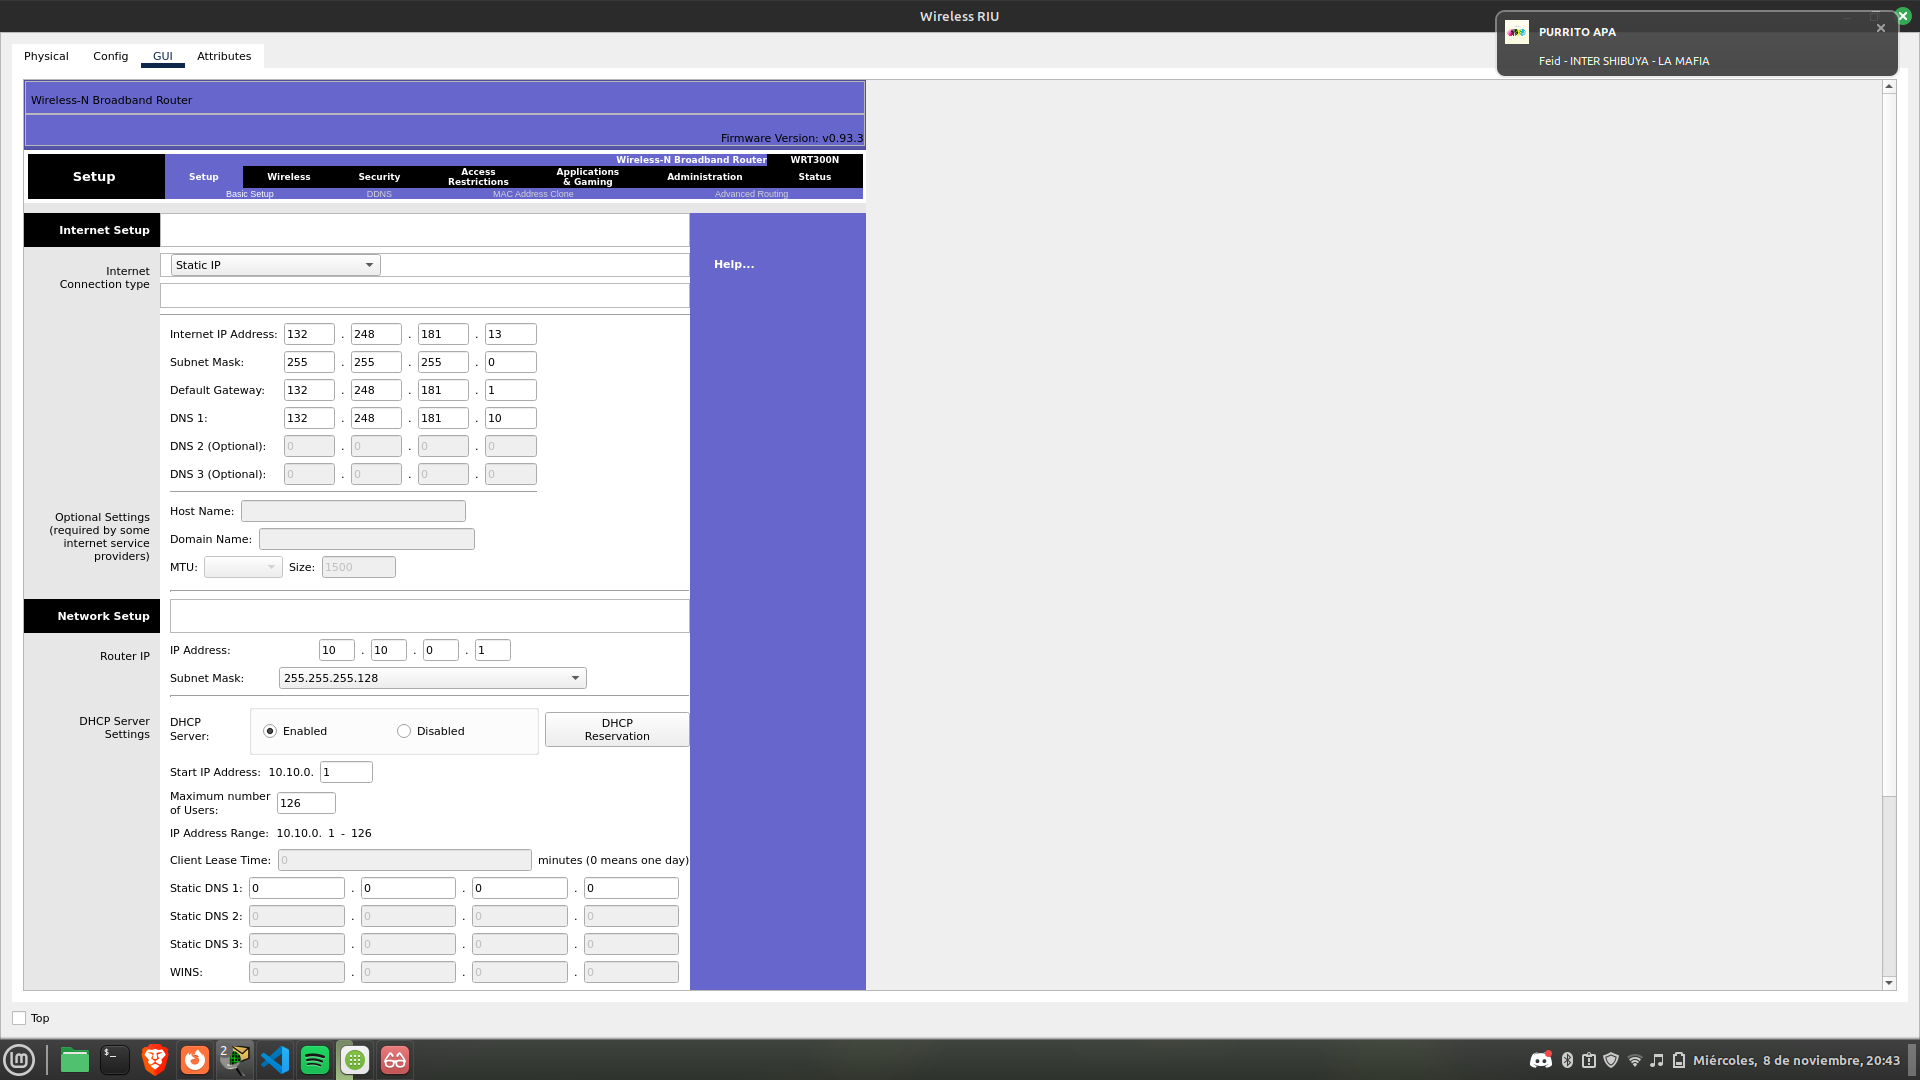
\includegraphics[width=12cm, height=8cm]{images/ima1.png} 

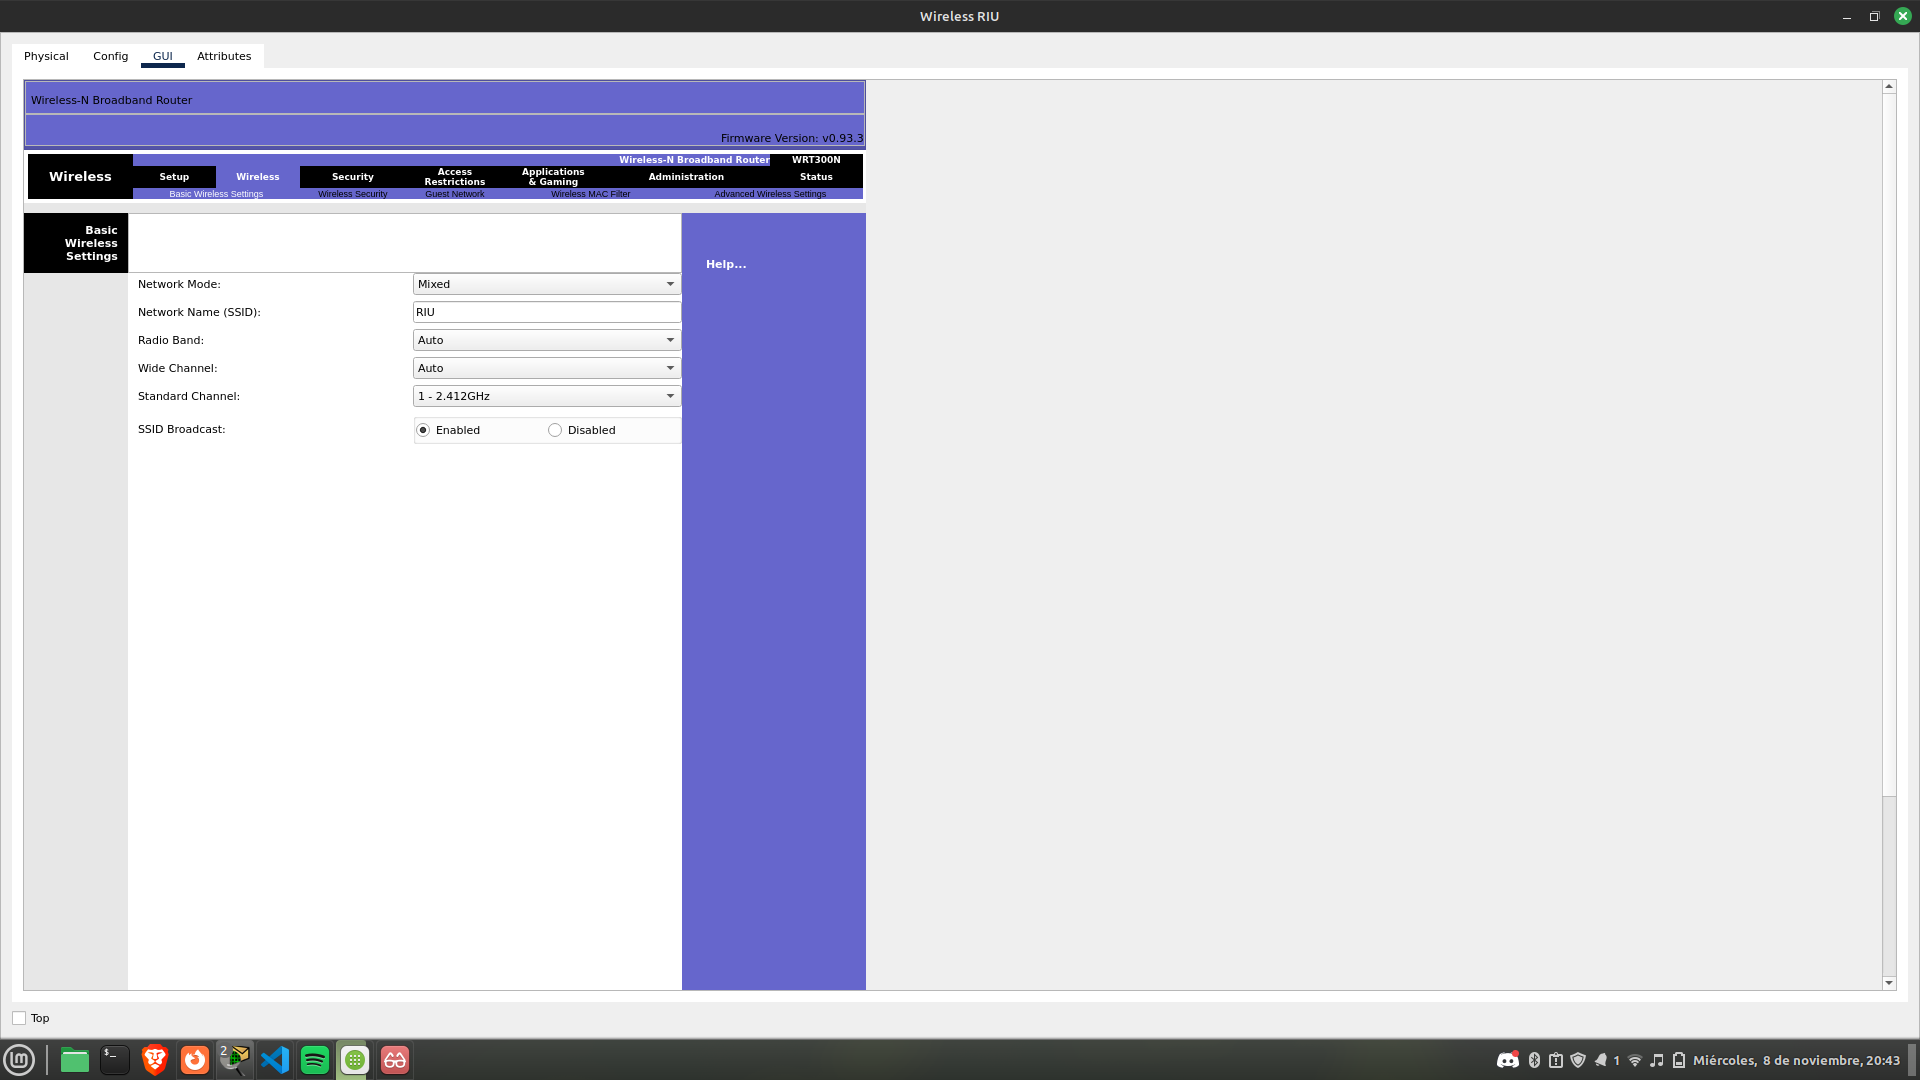
\includegraphics[width=12cm, height=8cm]{images/ima2.png}\\

Seguido de ello, agregamos 2 dispositivos, una laptop y un Smartphone, los cuales conectamos a la red, para la laptop agregamos primero una interfaz de red, para que se pueda conectar.\\


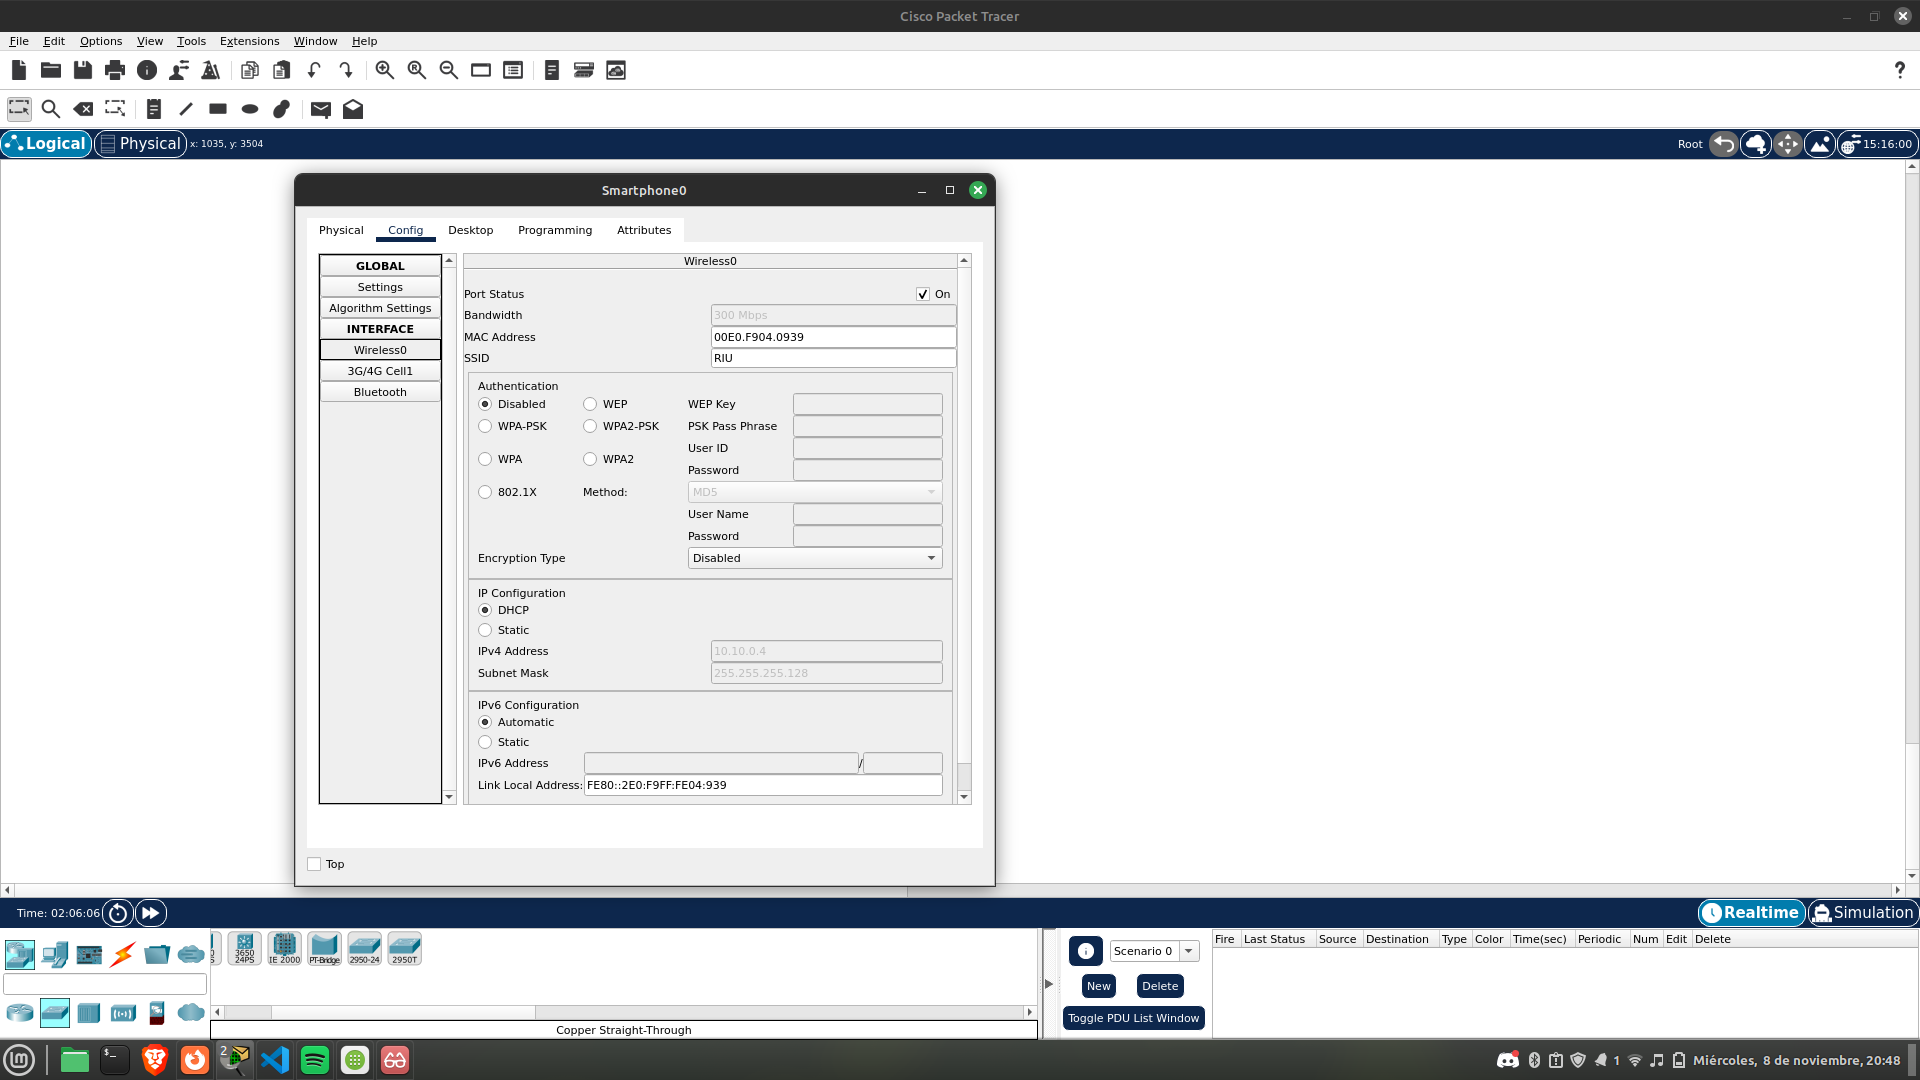
\includegraphics[width=12cm, height=8cm]{images/ima3.png}

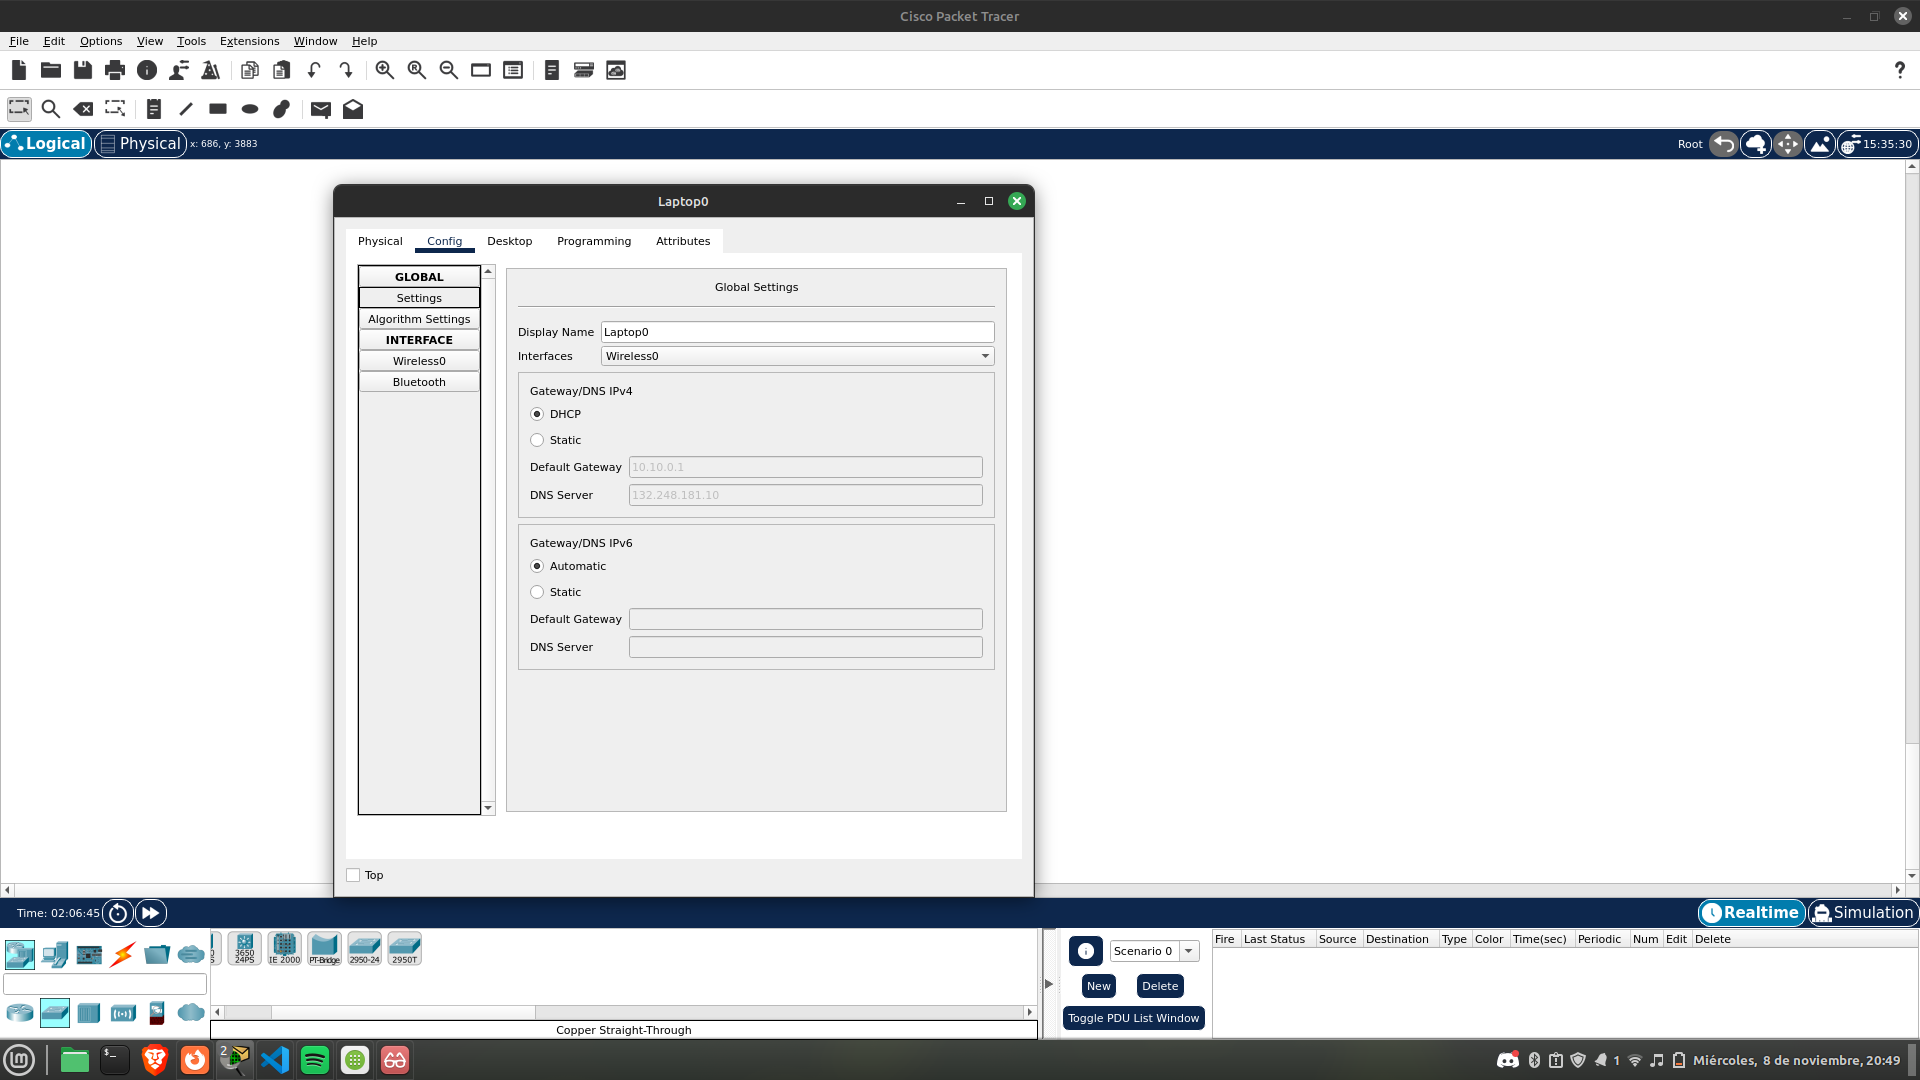
\includegraphics[width=12cm, height=8cm]{images/ima4.png}\\

Seguido de esto vamos a realizar la configuración de un servidor web.
Este servidor web tendra los parametros especificos que se muestran en el pdf de la practica. A continuación mostrare las configuraciones correspondientes.\\

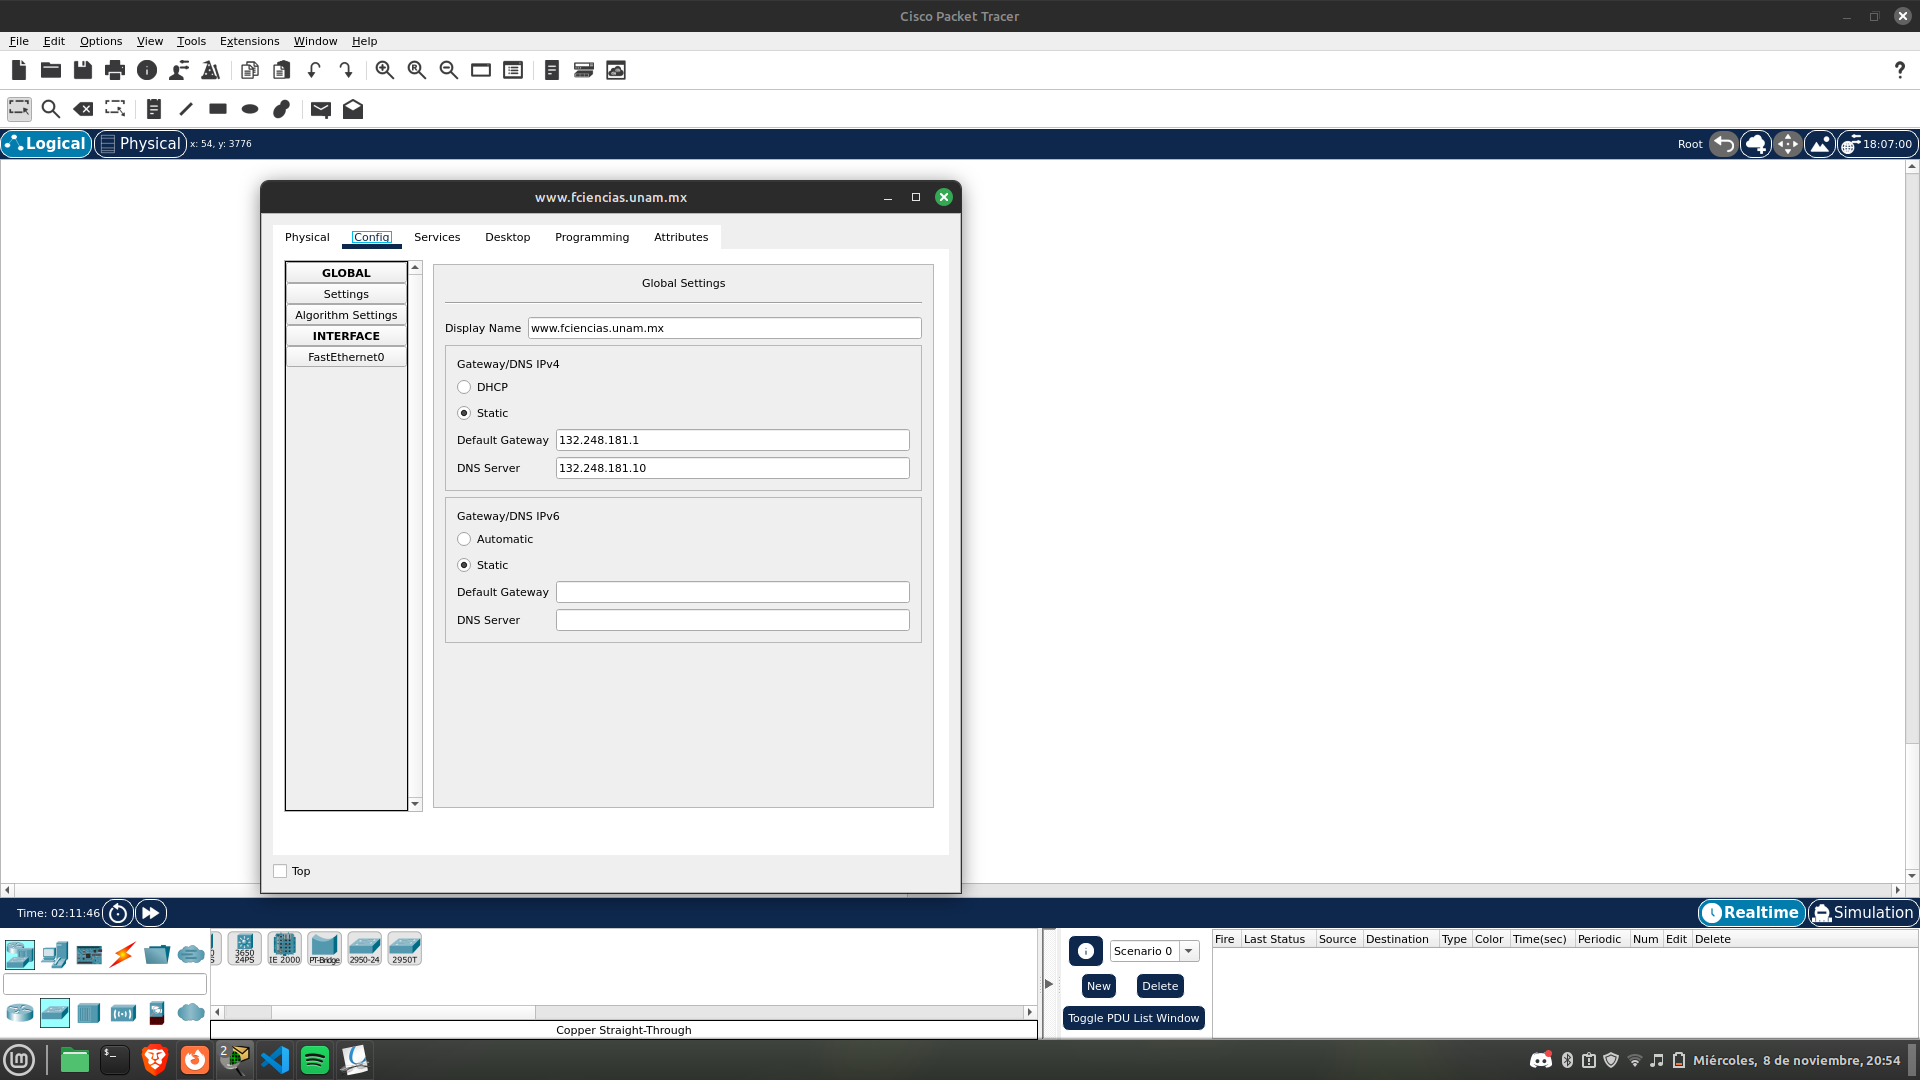
\includegraphics[width=12cm, height=8cm]{images/ima5.png}

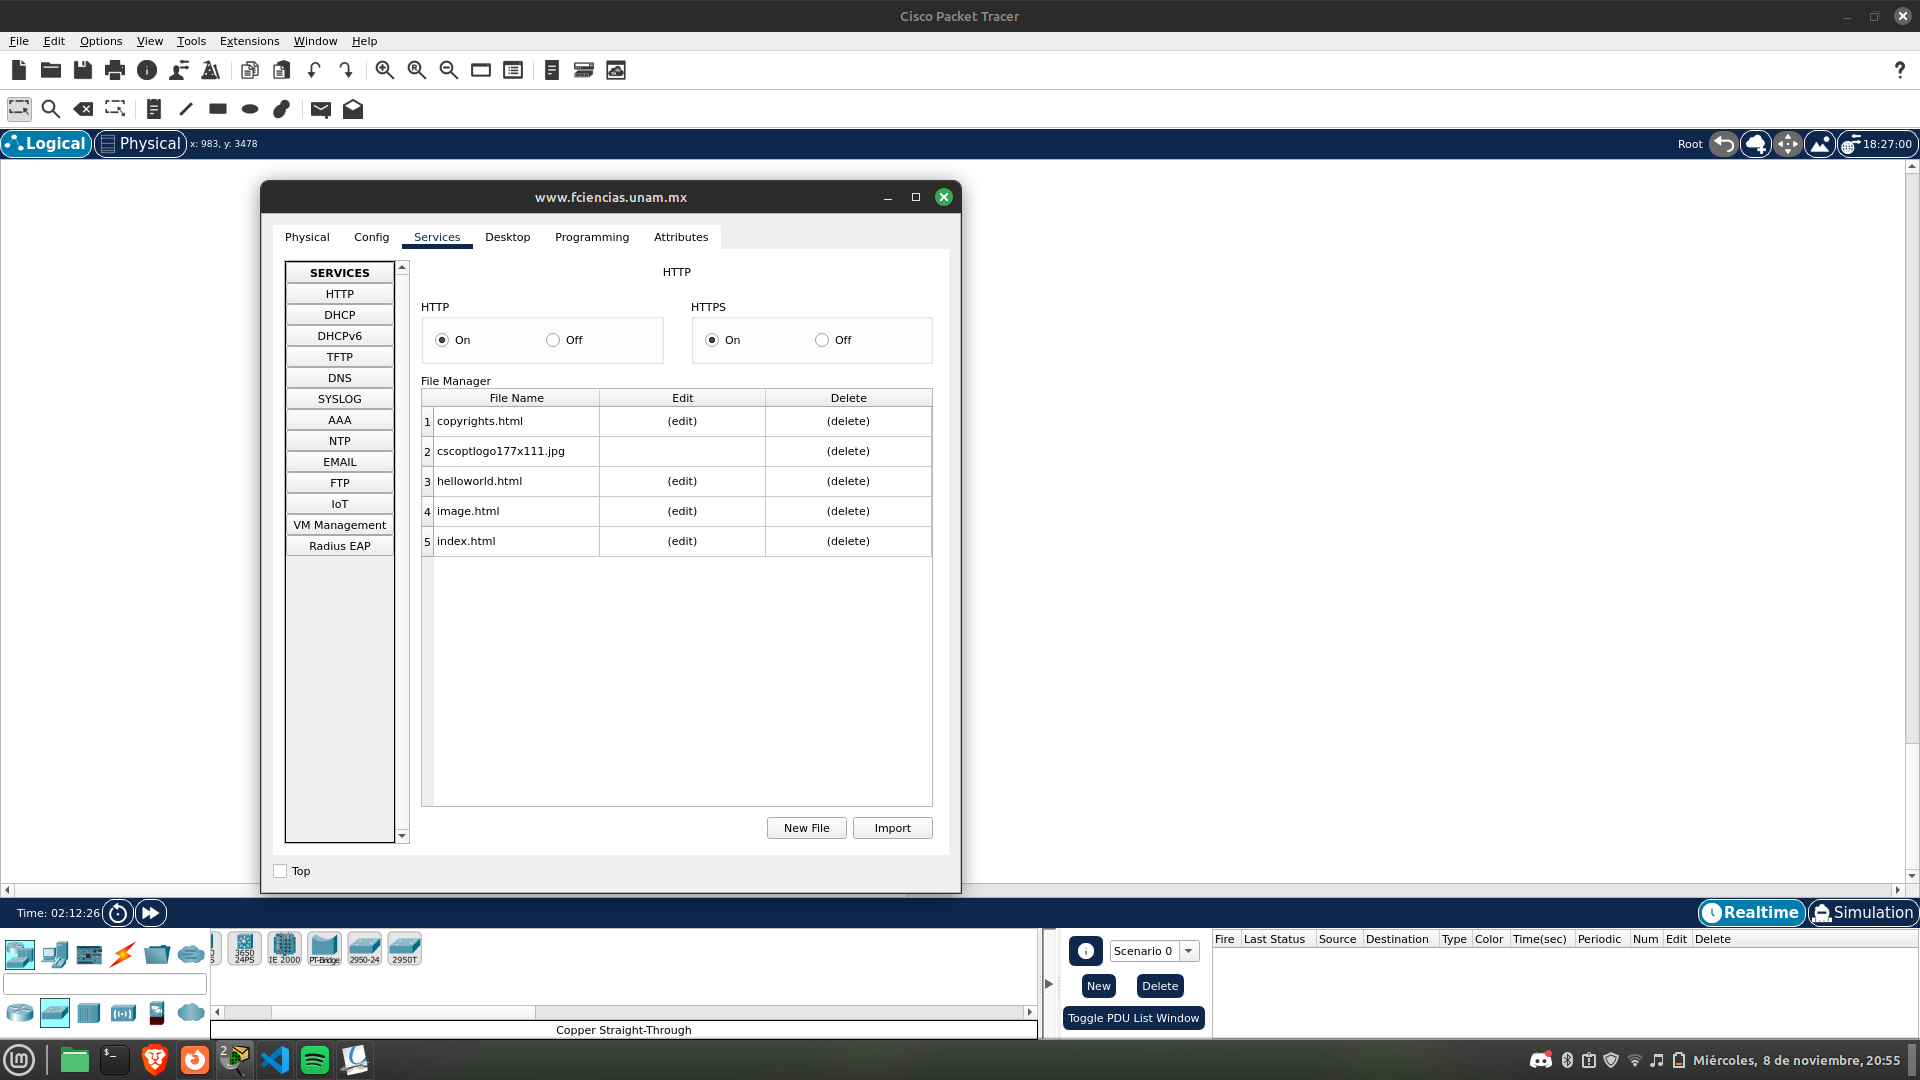
\includegraphics[width=12cm, height=8cm]{images/ima6.png}\\

Tambien configuramos un servidor DNS con las siguientes caracteristicas:\\

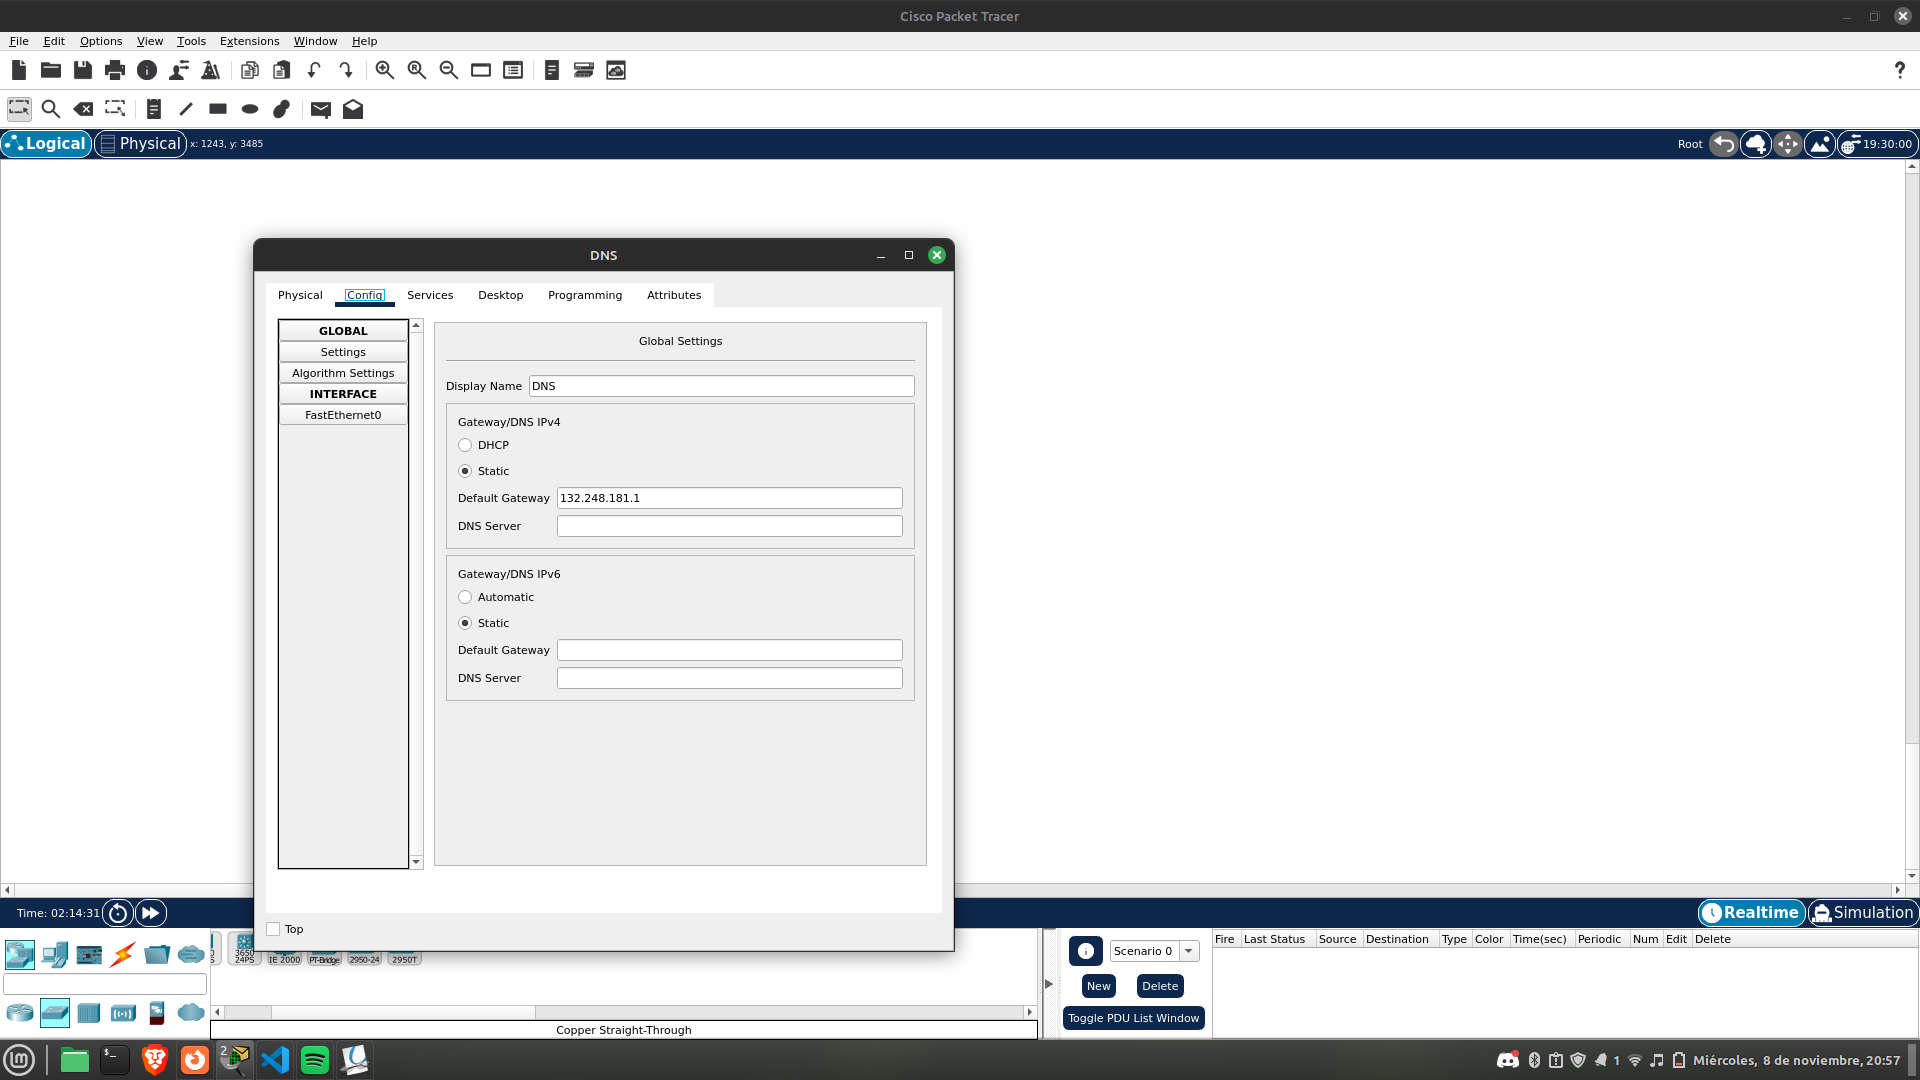
\includegraphics[width=12cm, height=8cm]{images/ima7.png}

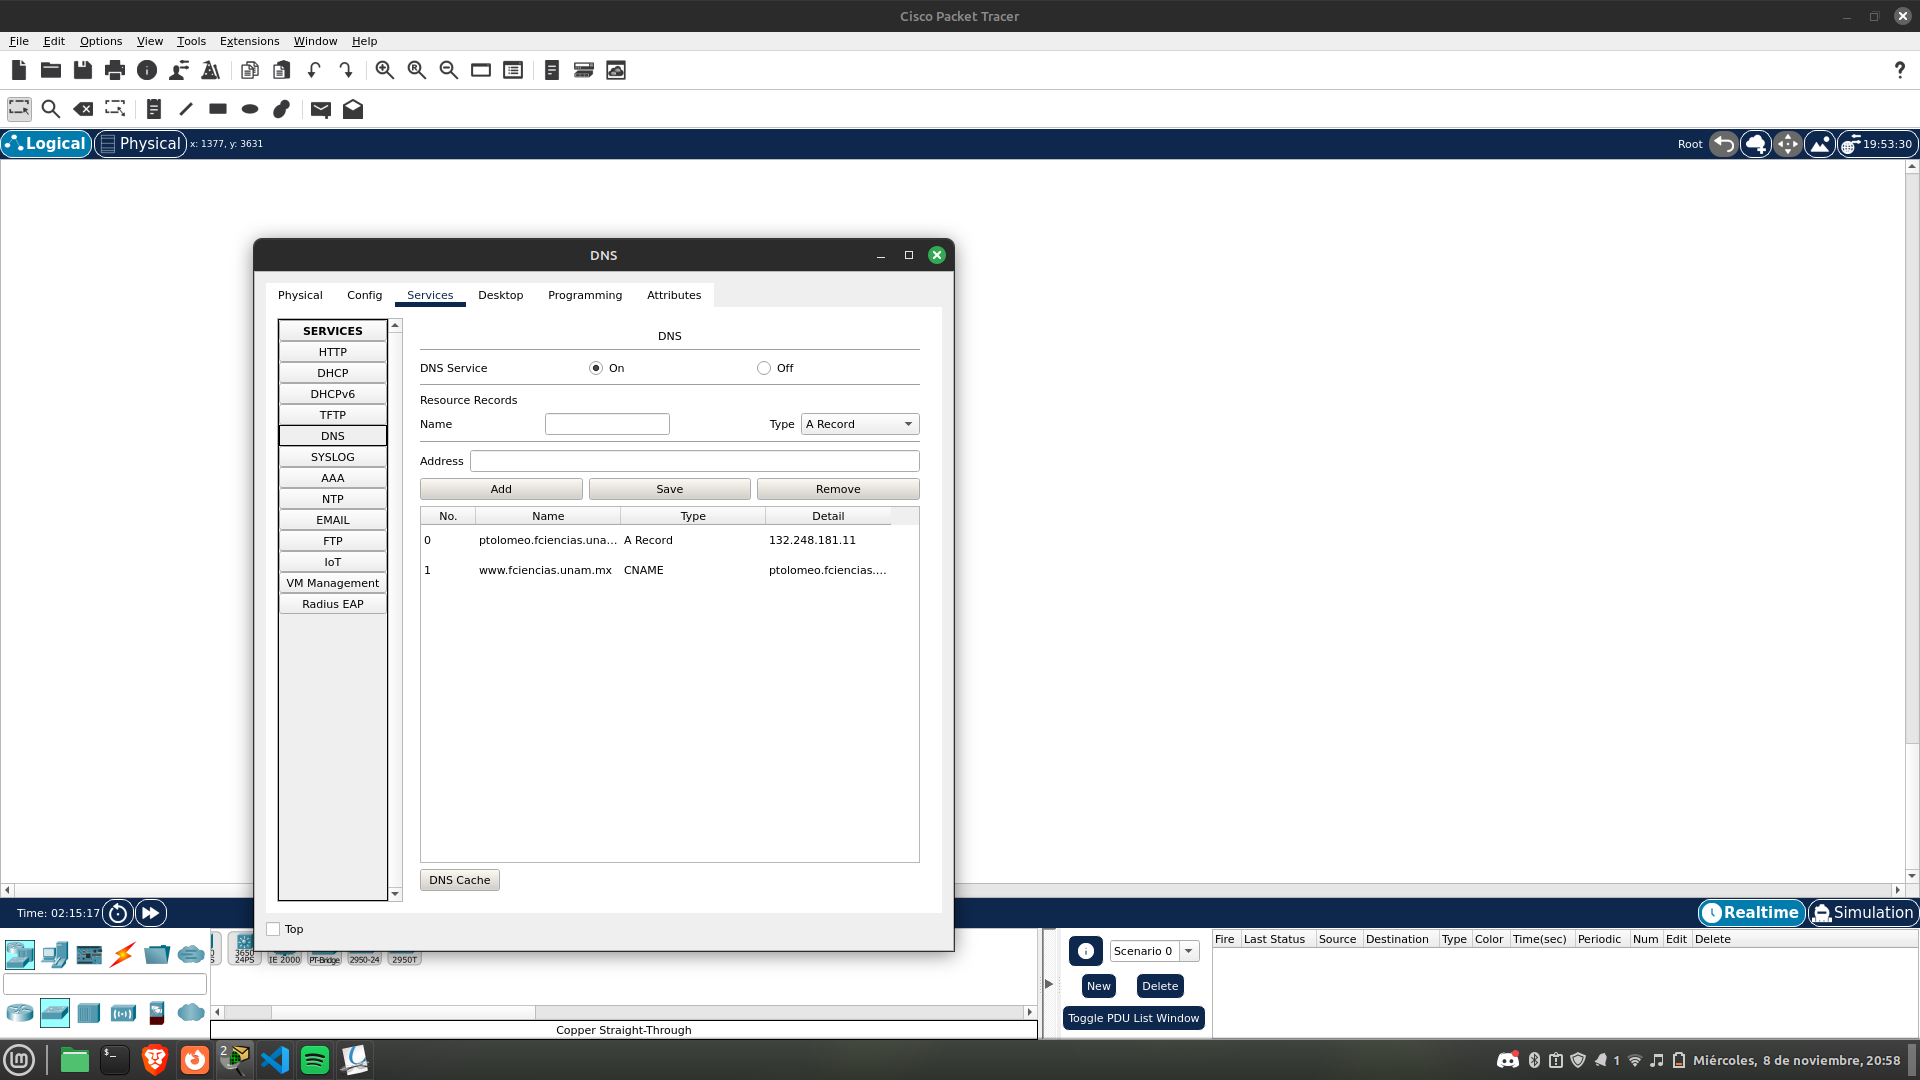
\includegraphics[width=12cm, height=8cm]{images/ima8.png}\\

Ahora lo que haremos es conectar los servidores con la RIU y esto lo hacemos dado el diagrama principal, mediante un Switch2950-24. Como lo mostramos a continuación.\\

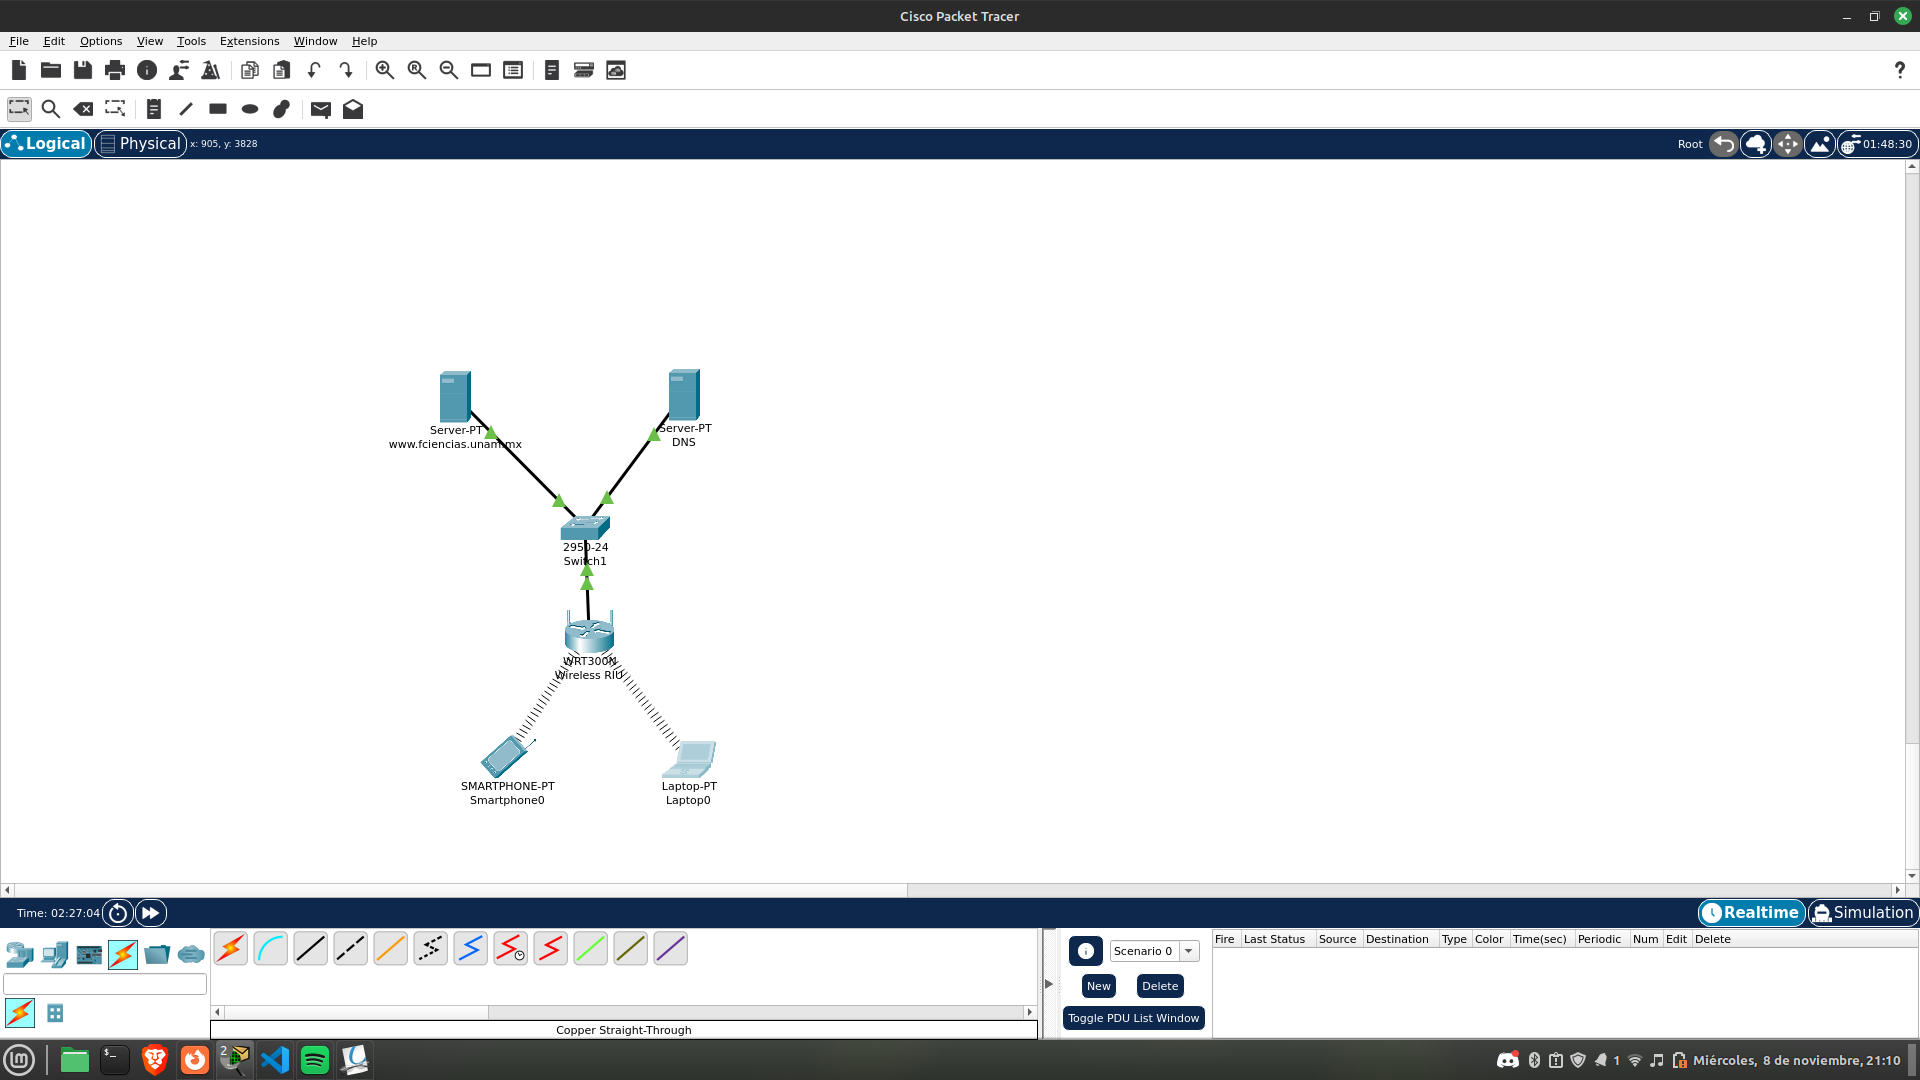
\includegraphics[width=12cm, height=8cm]{images/ima9.png}\\

Ahora probamos que se pueda visualizar desde la laptop asi como desde el dispositivo movil.\\

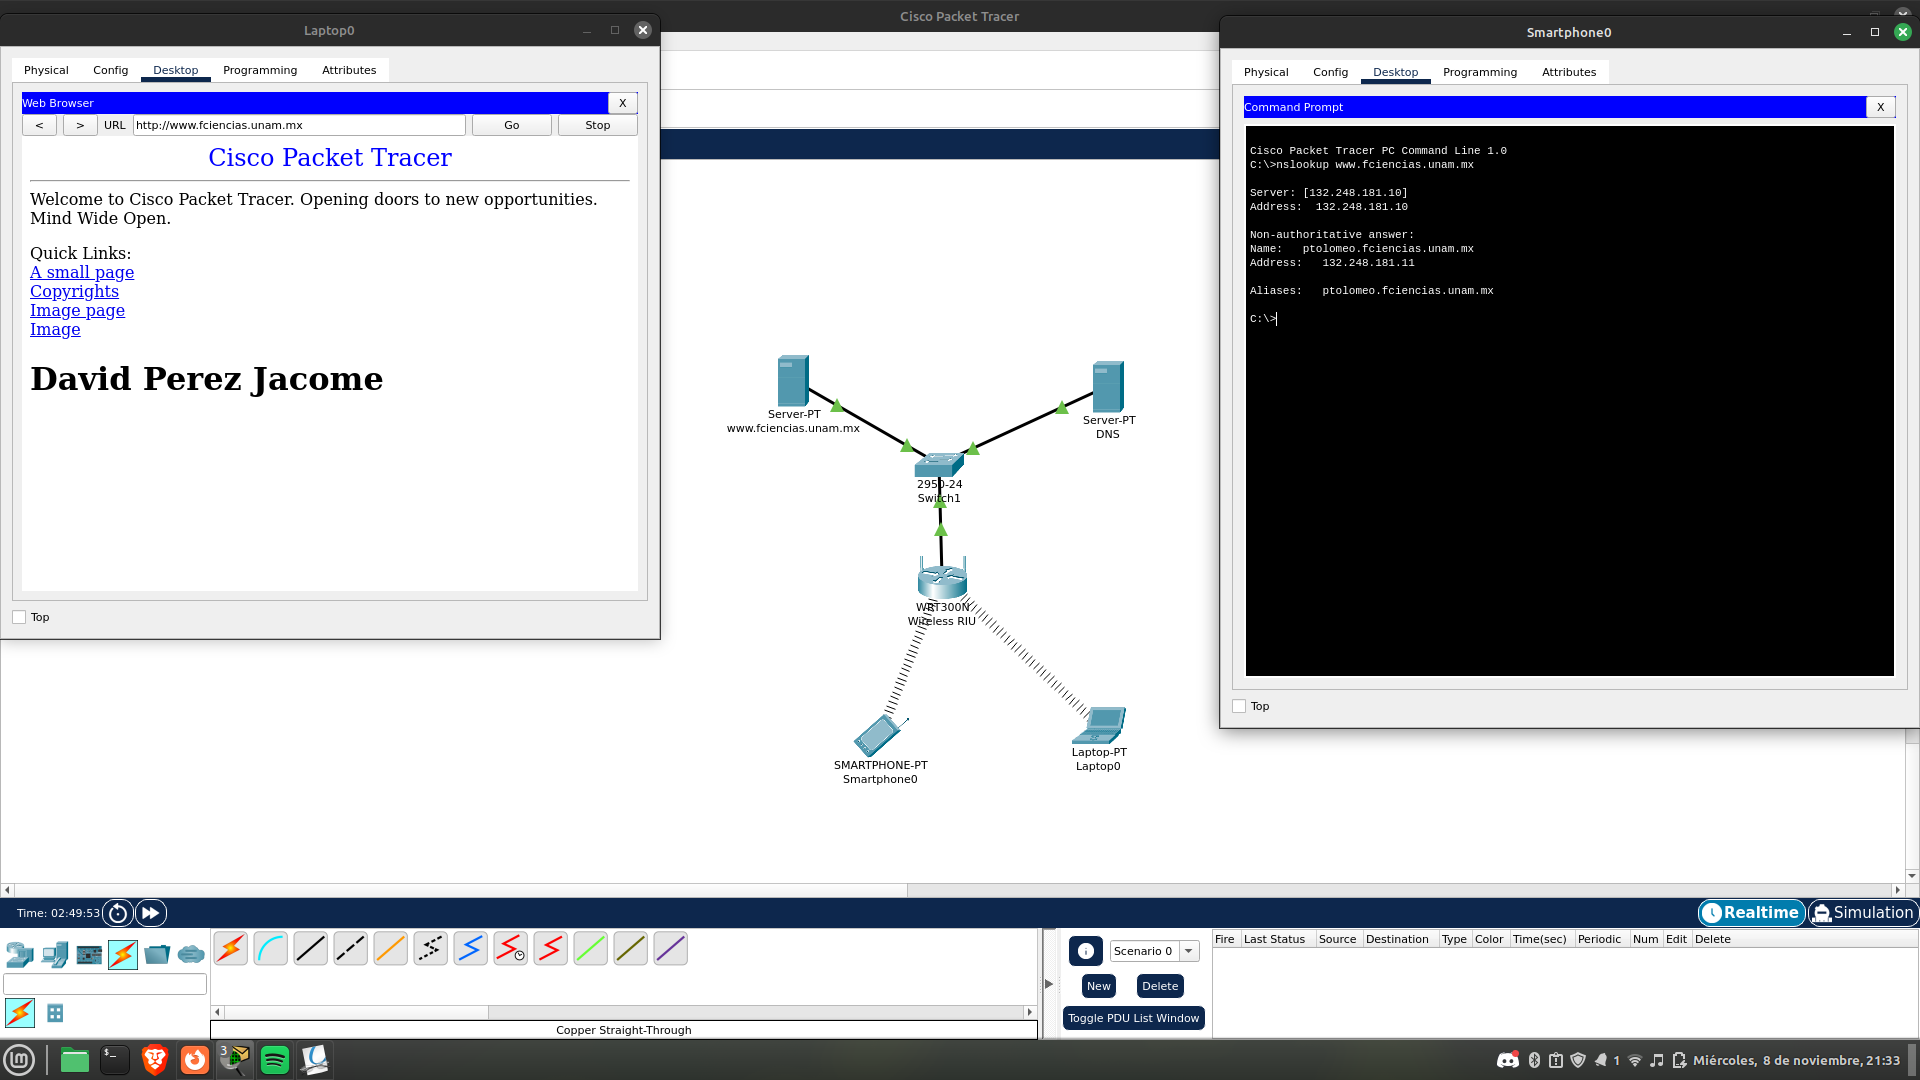
\includegraphics[width=12cm, height=8cm]{images/prueba de web y smartfphone.png}\\

{\color{red} \subsubsection*{\textbf{Configuración de red de laboratorio A}}}
\vspace{1em}

Ahora vamos a configuarar un servidor DHCP, como se muestra a continuacion:\\

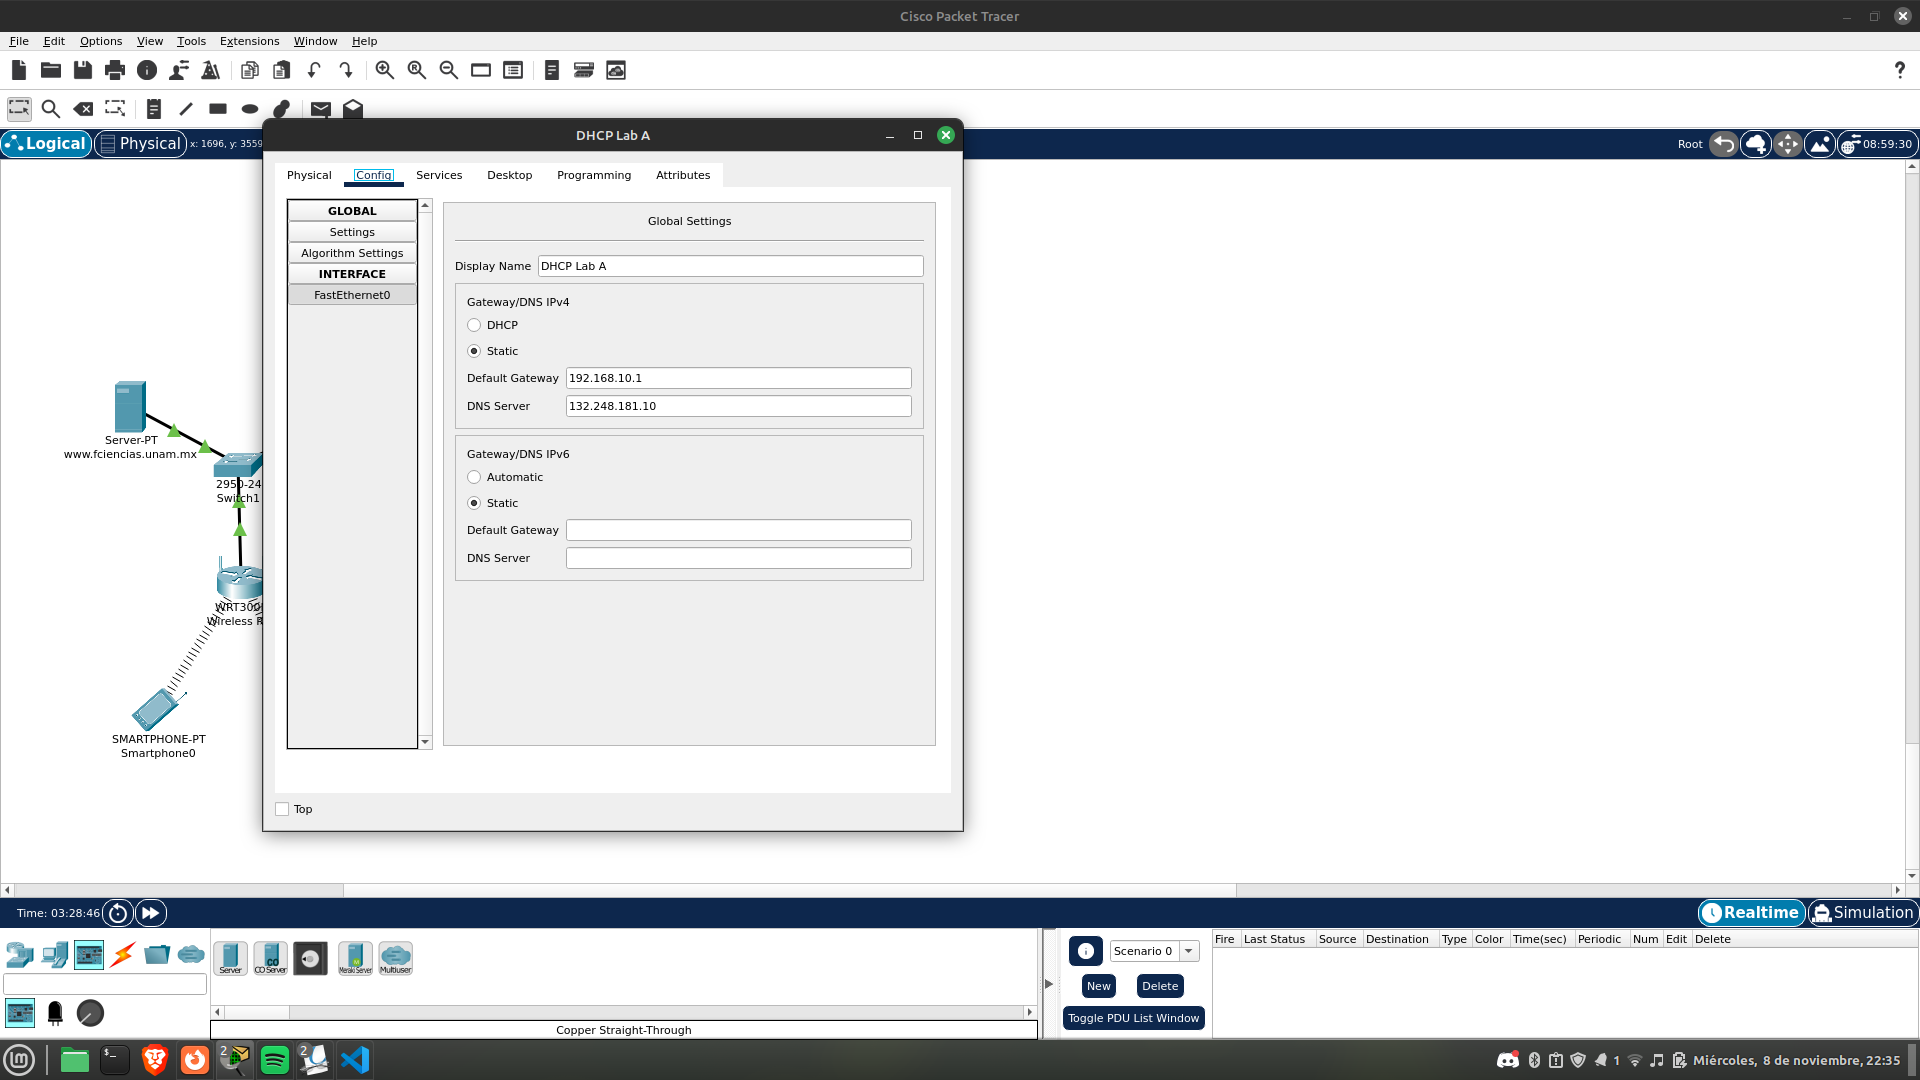
\includegraphics[width=12cm, height=8cm]{images/dhcp1.png}

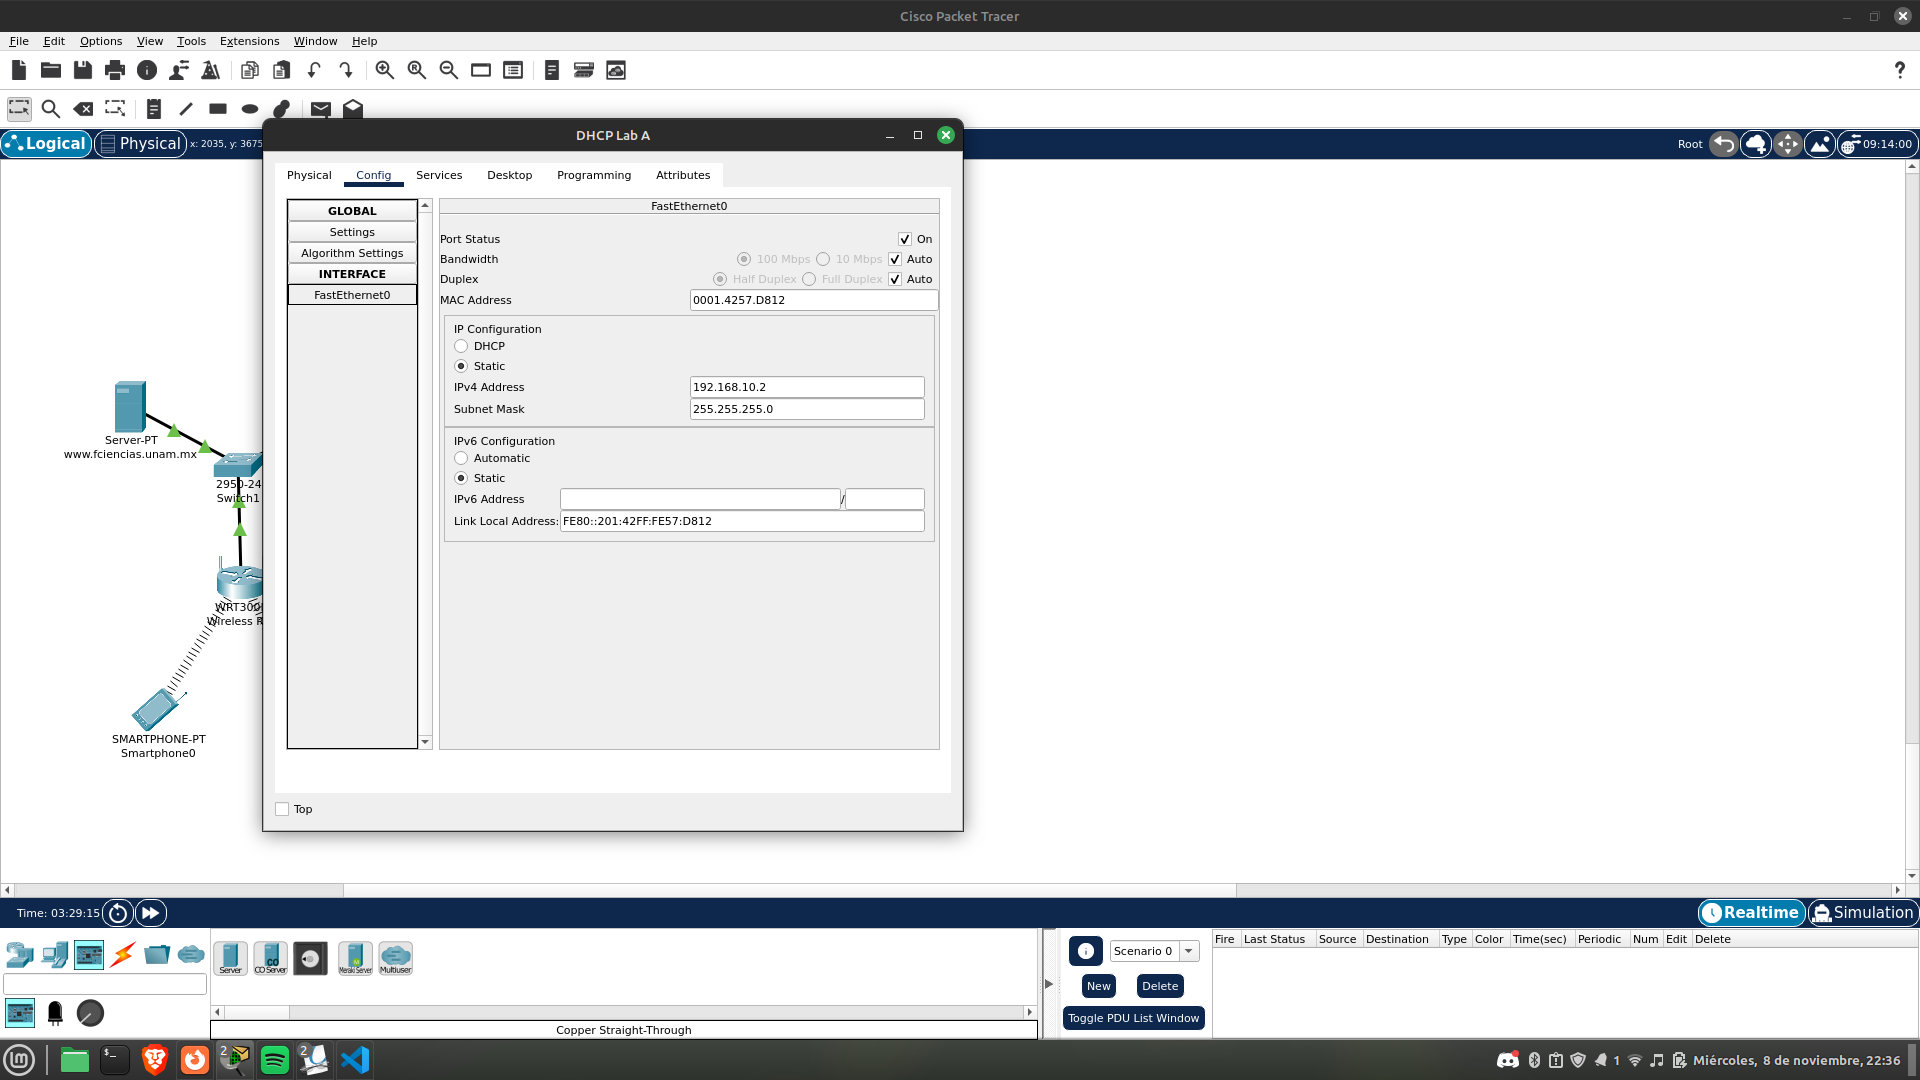
\includegraphics[width=12cm, height=8cm]{images/dhcp2.png}

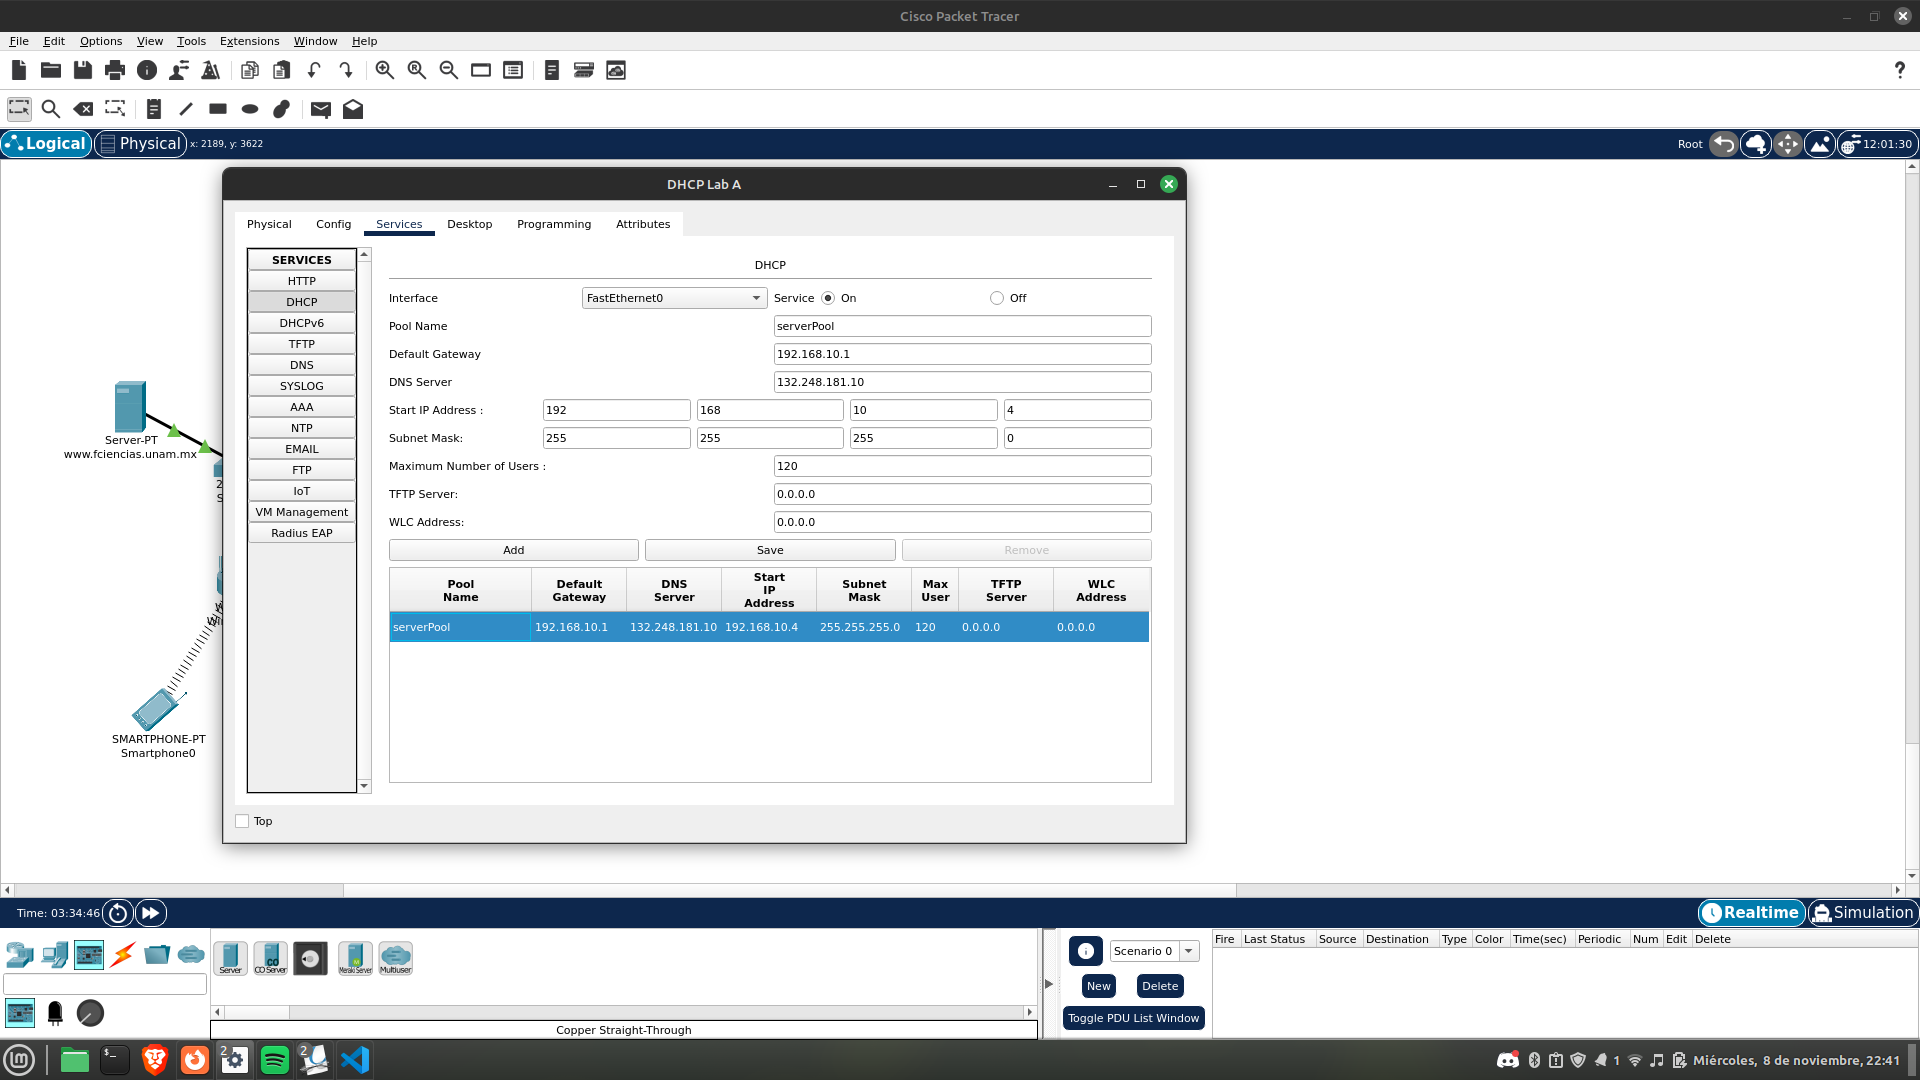
\includegraphics[width=12cm, height=8cm]{images/dhcp3.png}\\

Ahora configuaramos la impresora Printer lab A con los siguientes parametros:\\

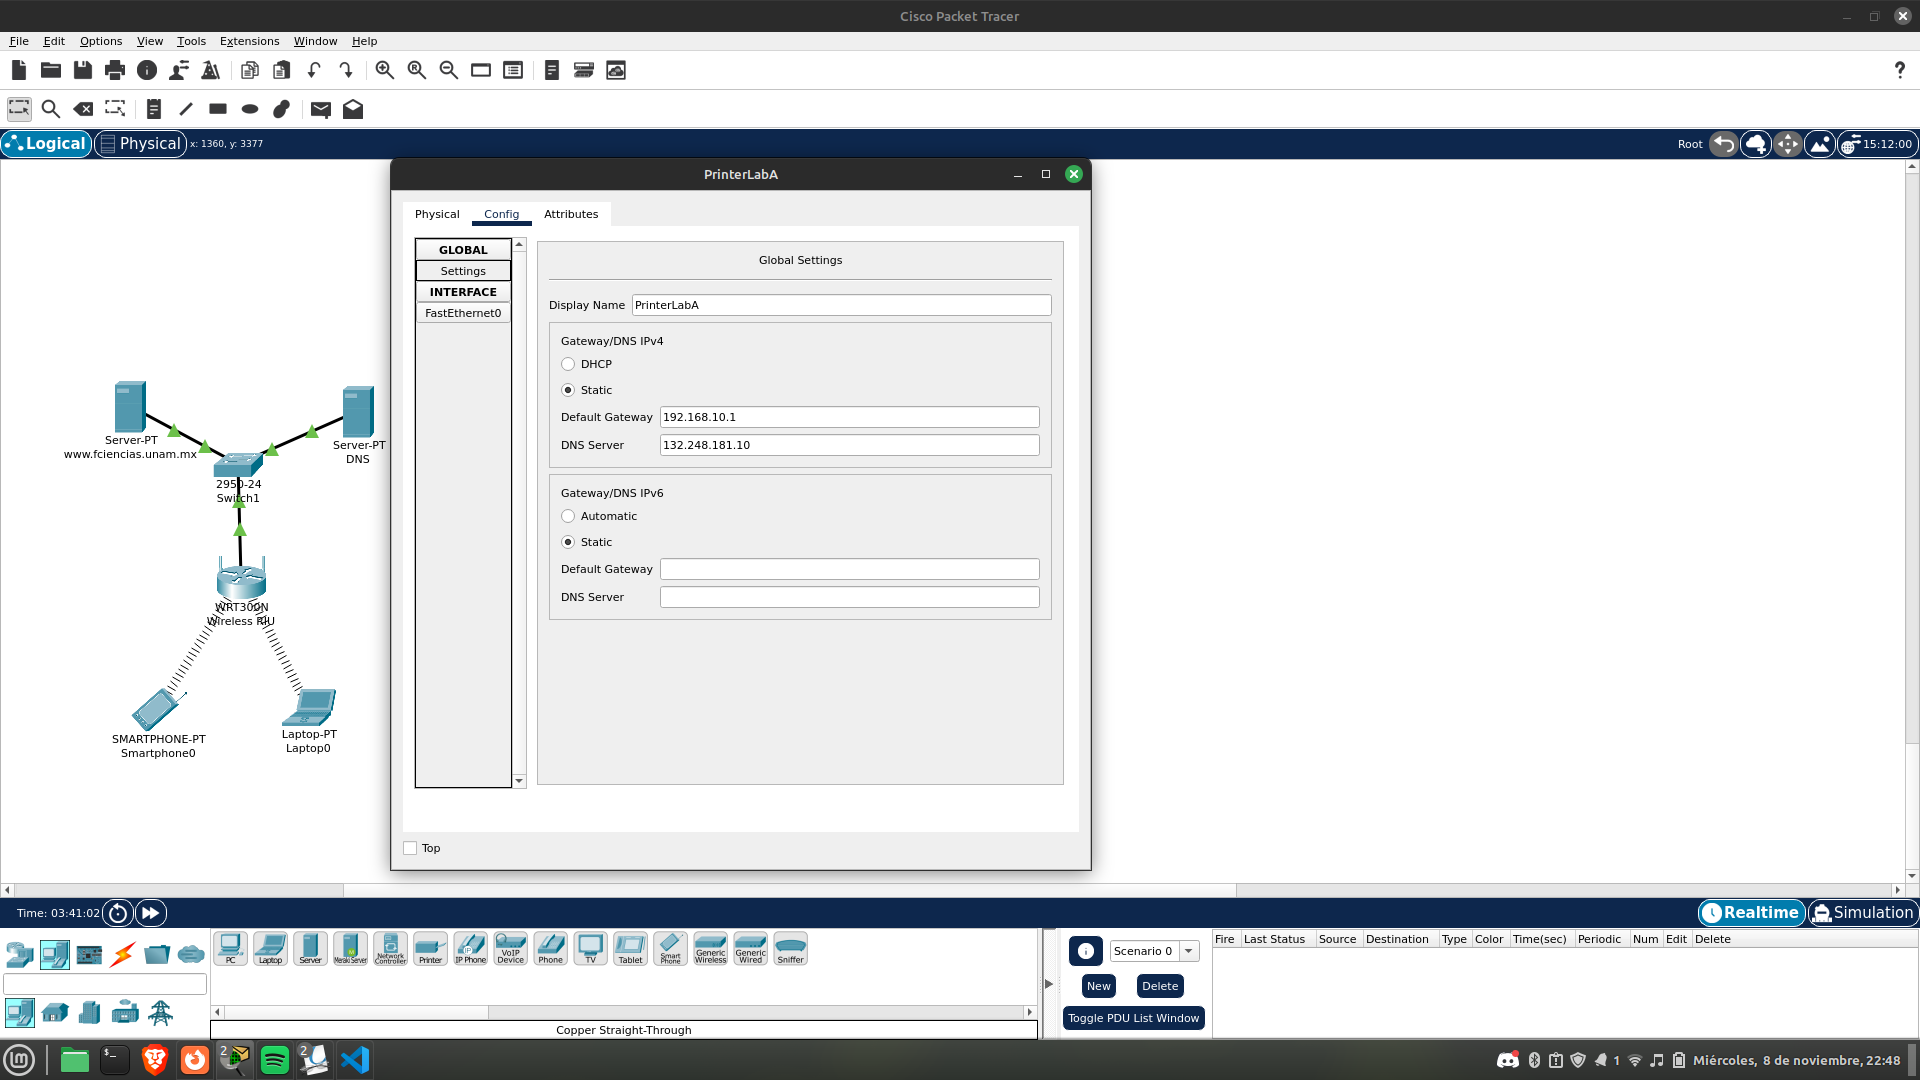
\includegraphics[width=12cm, height=8cm]{images/impresoralaba.png}

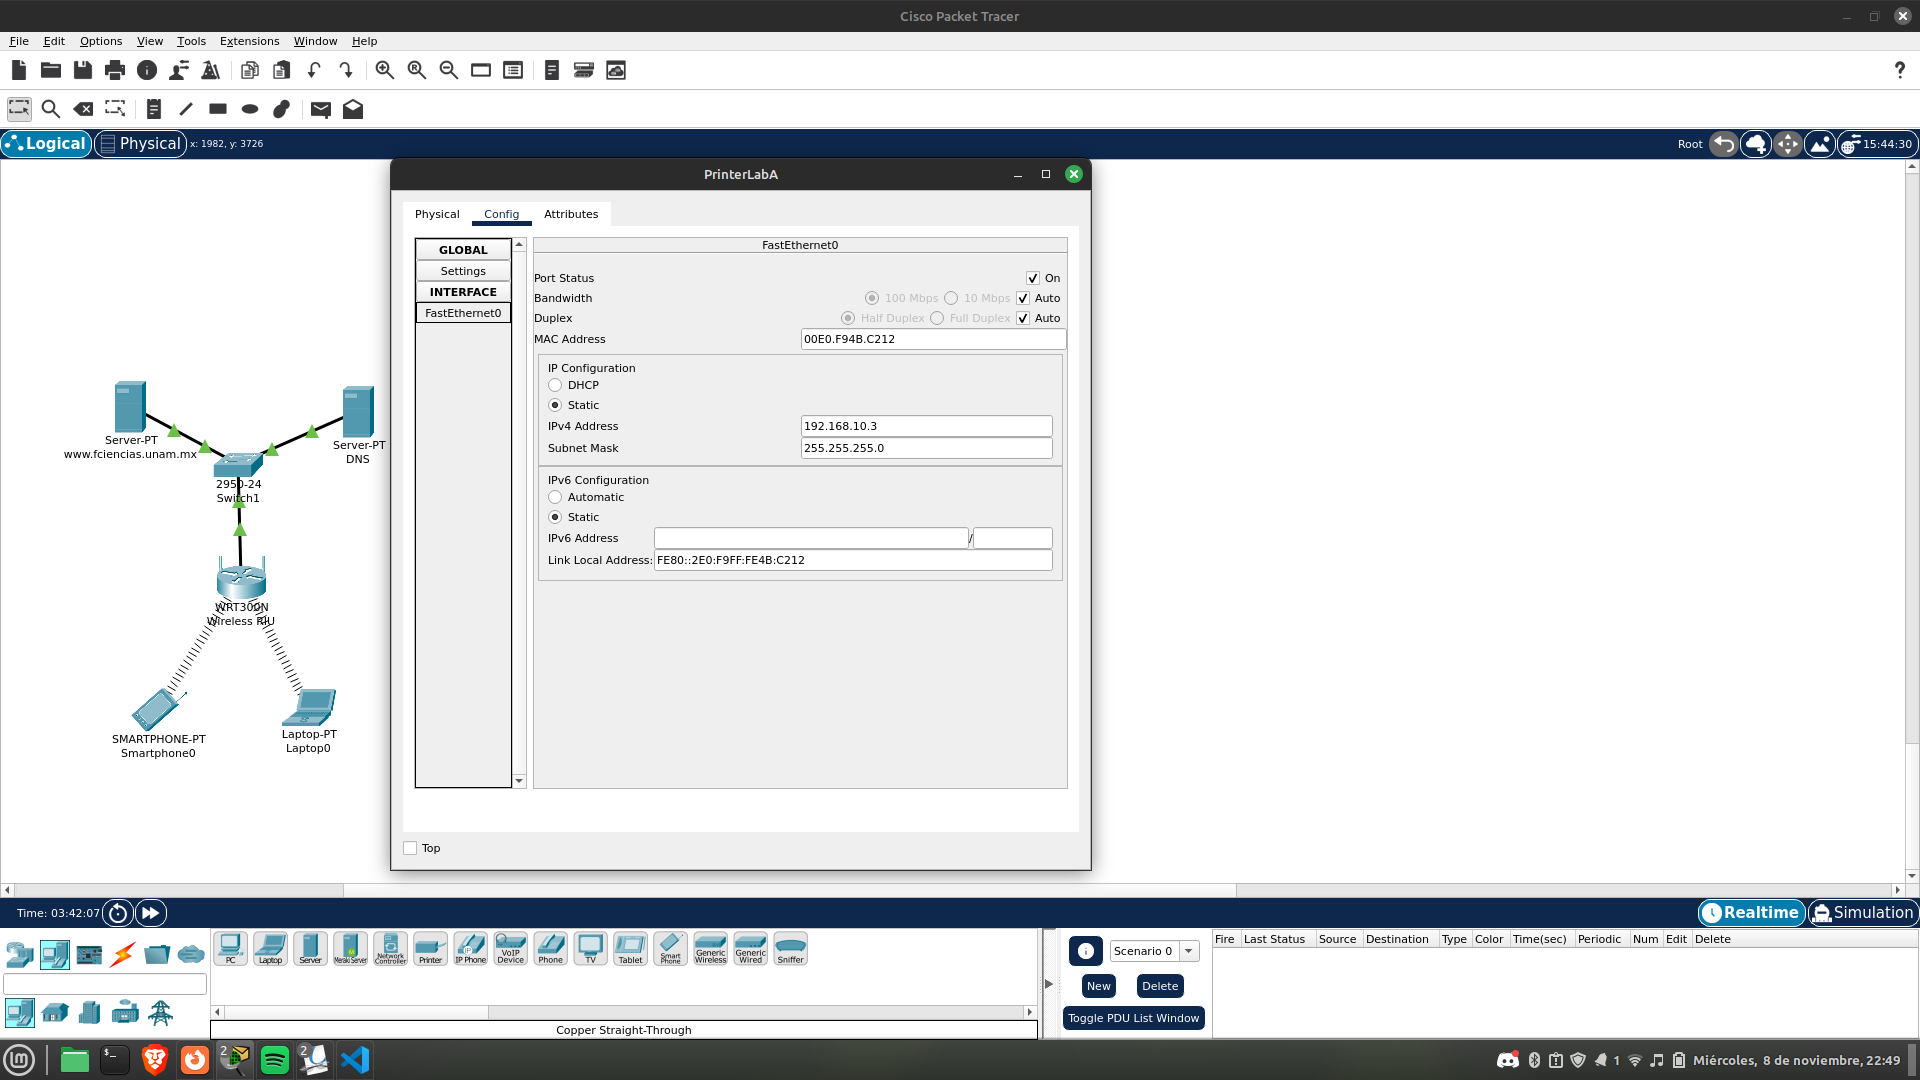
\includegraphics[width=12cm, height=8cm]{images/impresoralaba2.png}\\

Además agregaremos 2 computadoras a este laboratorio y que el DHCP le asigne parametros de conexion de red\\

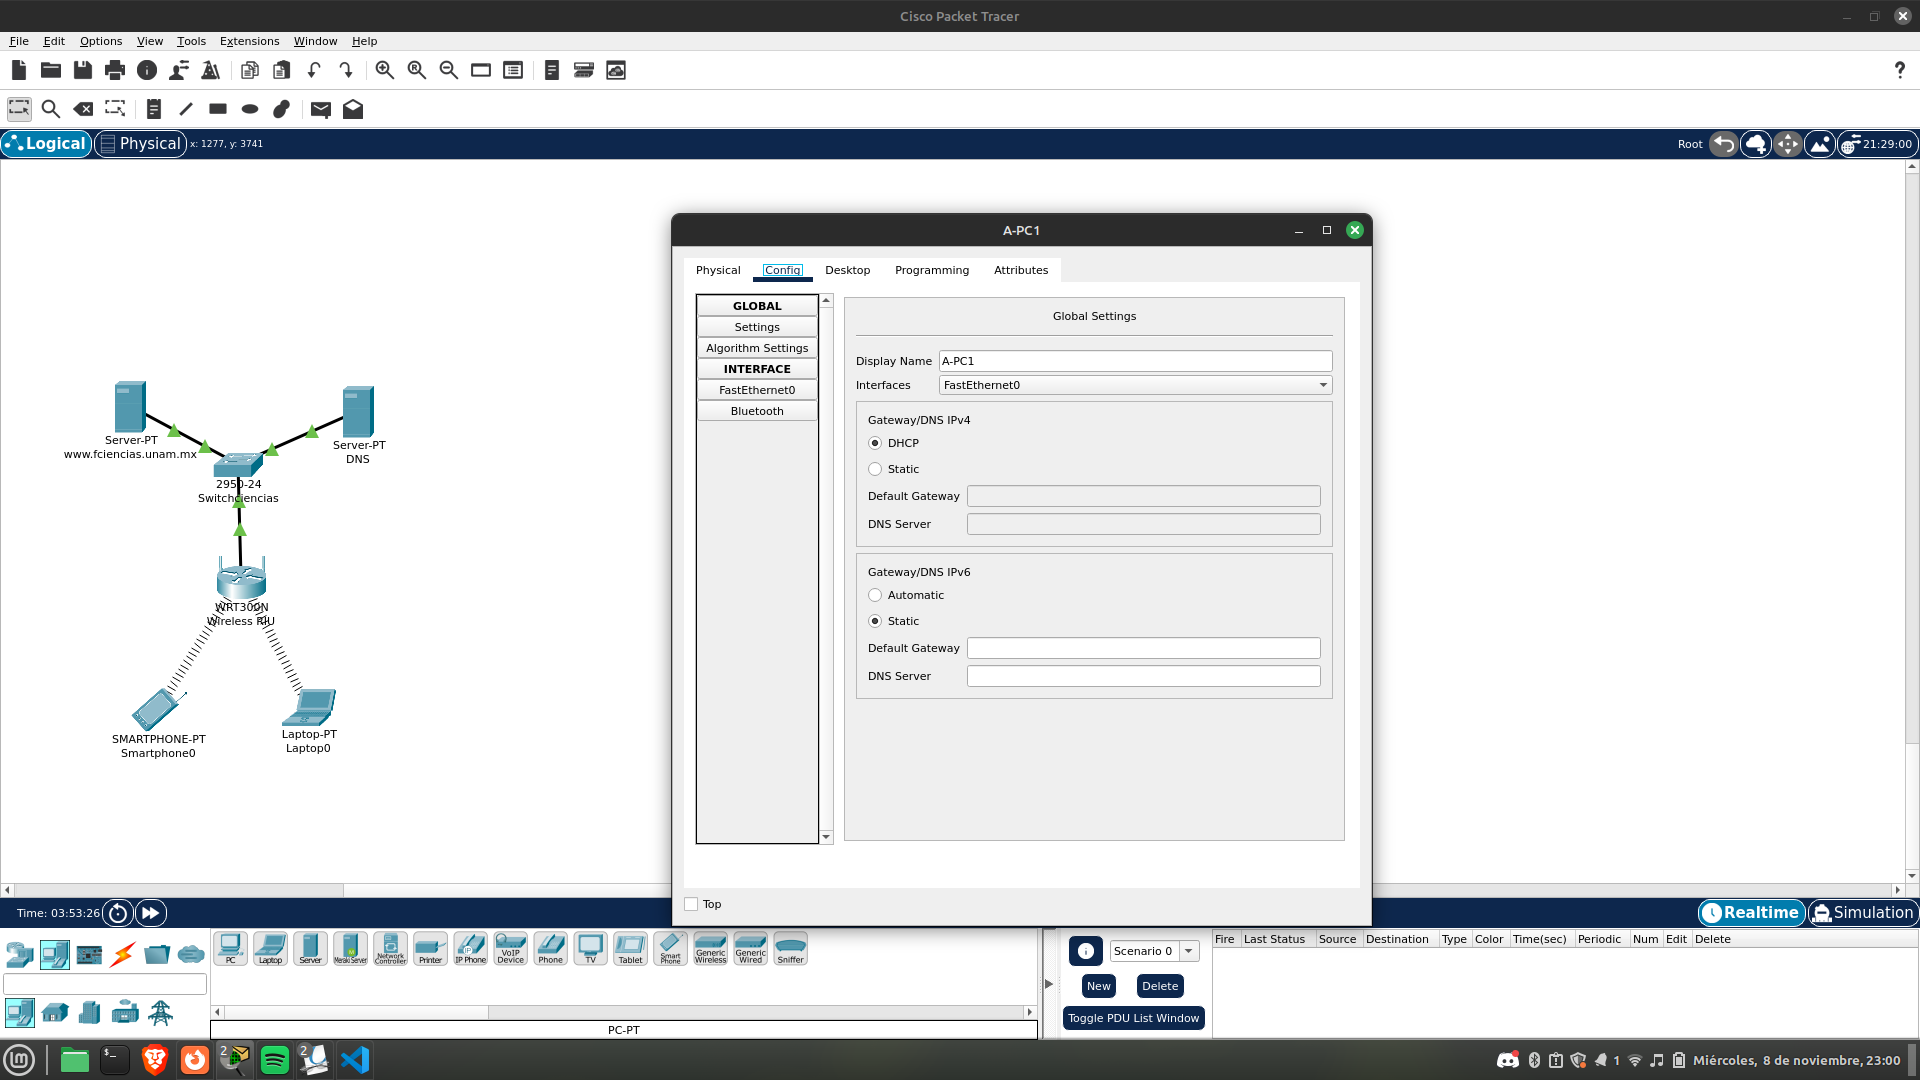
\includegraphics[width=12cm, height=8cm]{images/compus laba.png}\\

{\color{red} \subsubsection*{\textbf{Configuración del NAT/PAT para el router de la red del Laboratorio A}}}
\vspace{1em}

configuramos las redes del router, ademas de agregar su respectivo dispositivo de red.\\

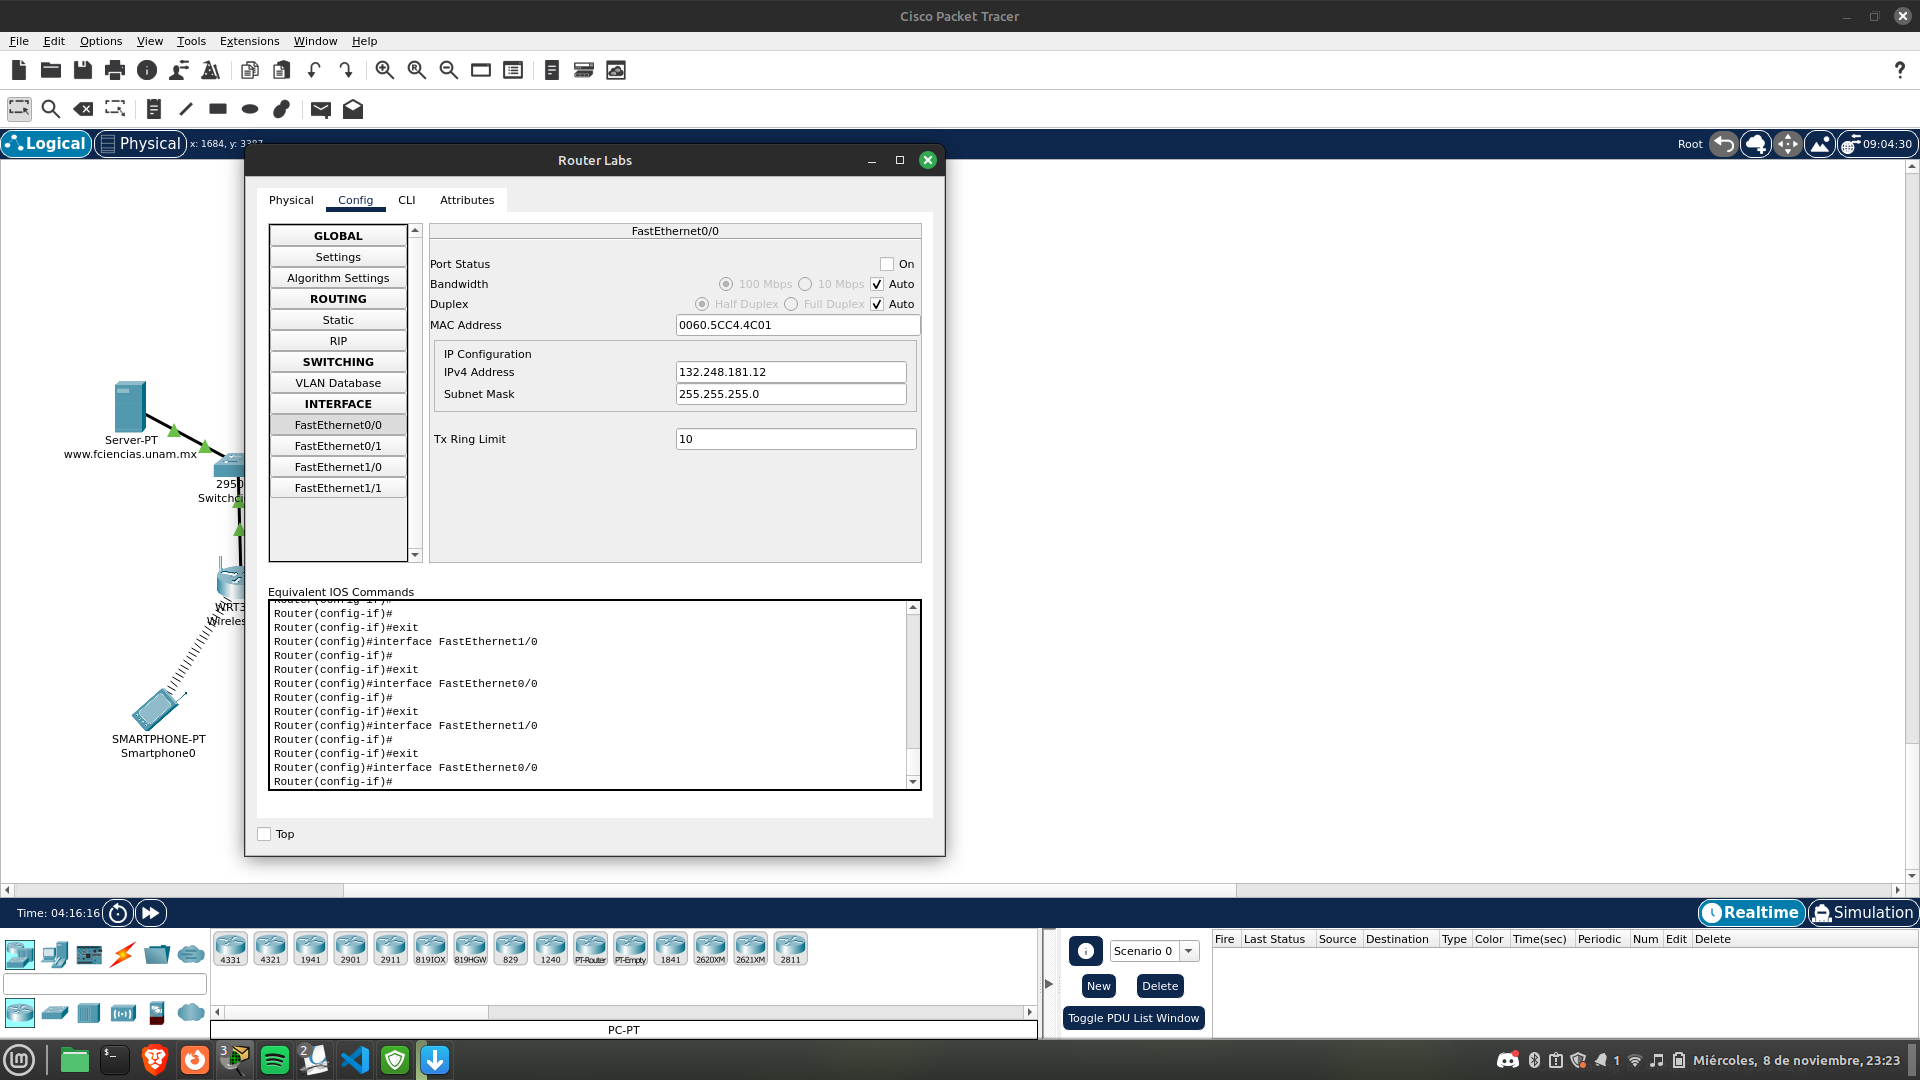
\includegraphics[width=12cm, height=8cm]{images/confirouterlab.png}\\

Seguido de eso conectamos el router de labs con un Switch2950 el cual a su vez debe de estar conectado con el DHCP Lab A, la impresora y las 2 computadoras.\\

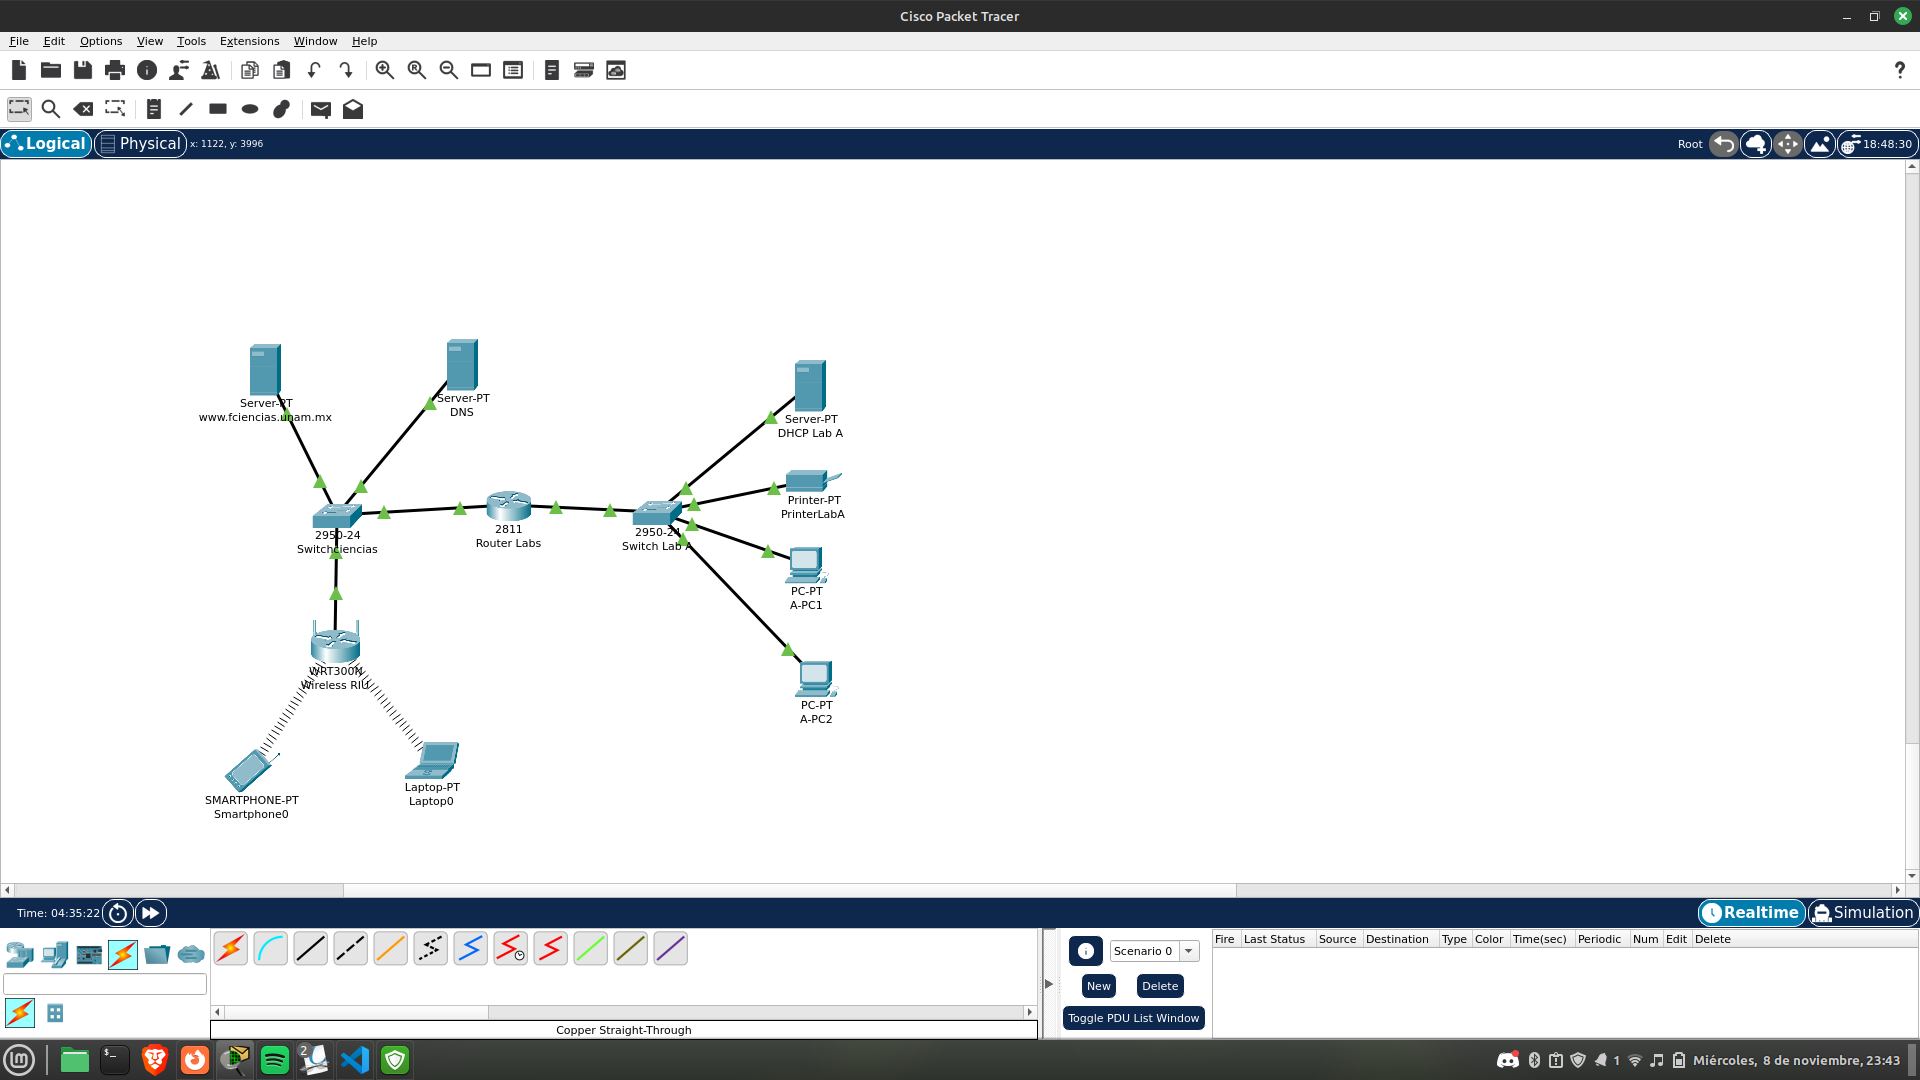
\includegraphics[width=12cm, height=8cm]{images/diagrama con laba.png}\\

Ahora probamos la conexión con la computadora 1 del laboratorio y es un exito:\\

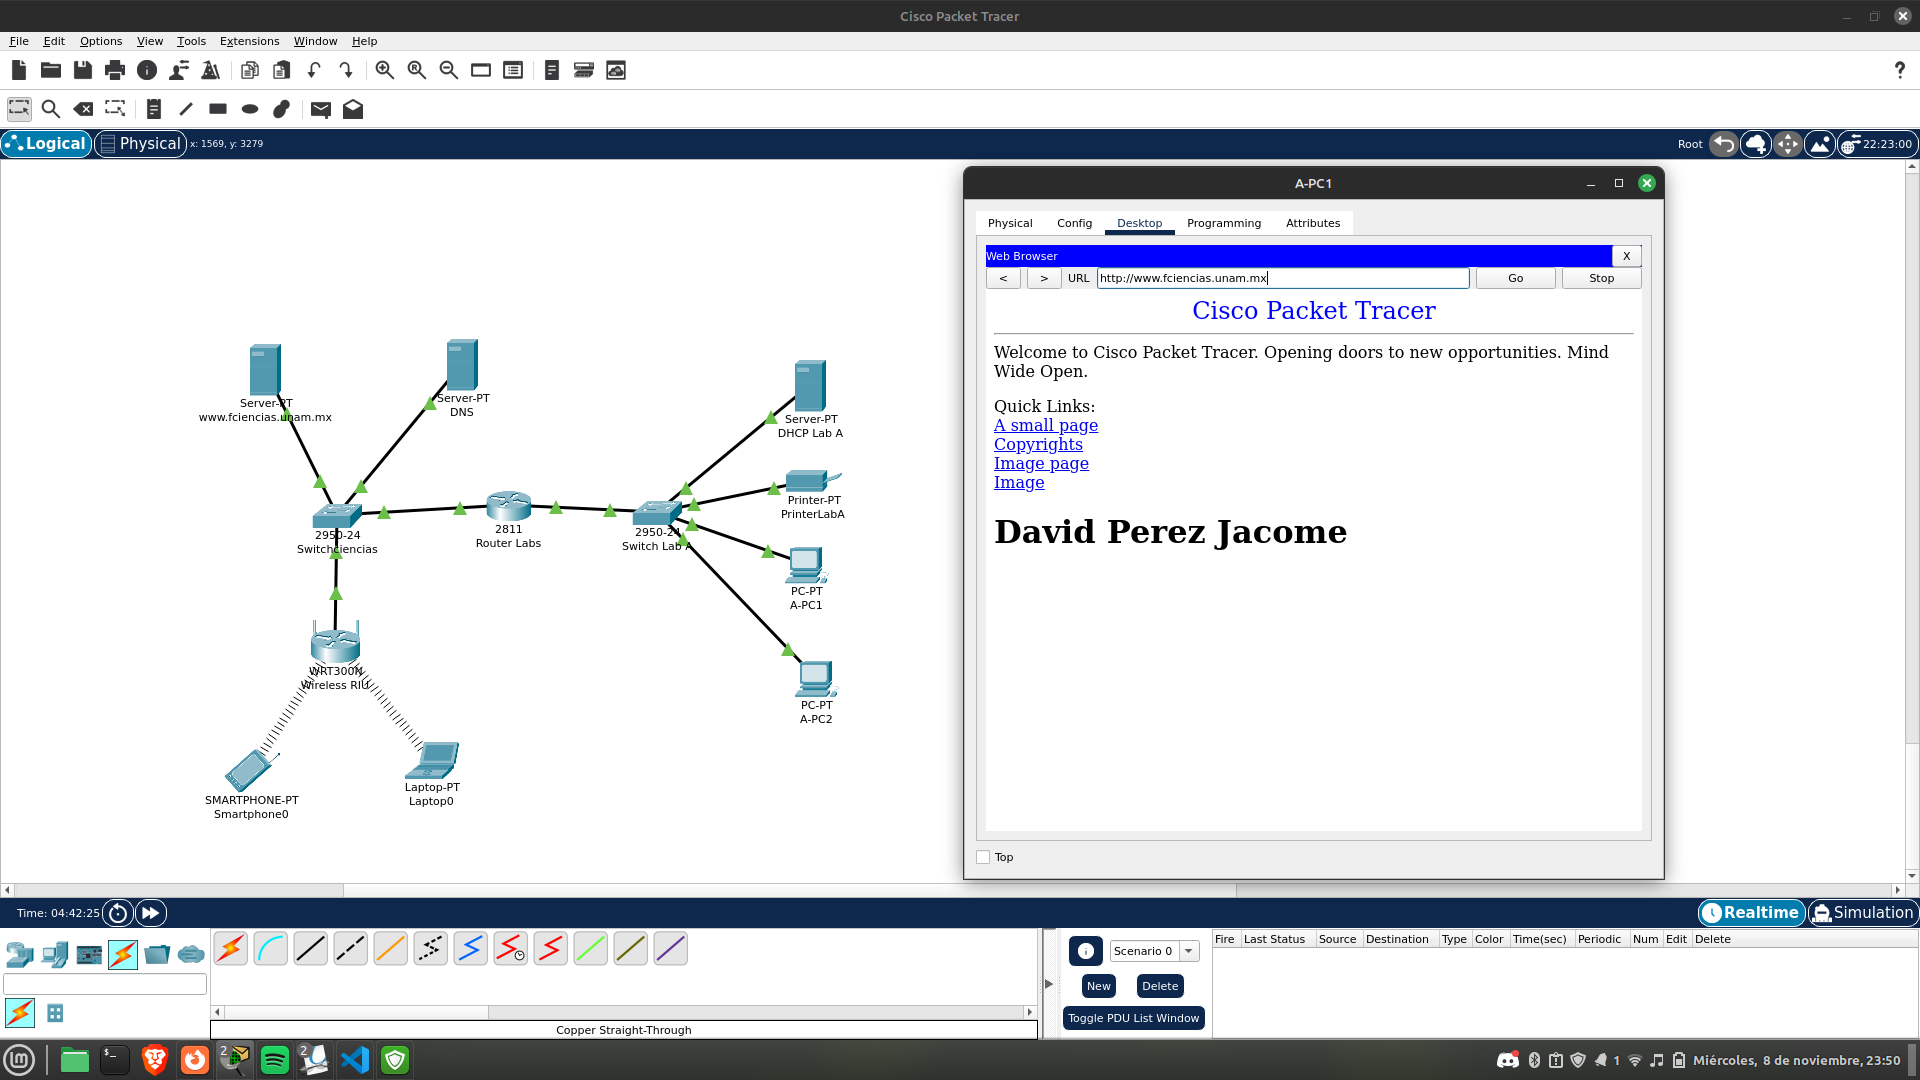
\includegraphics[width=12cm, height=8cm]{images/conexion laba.png}\\

Cabe mencionar que esta misma configuración la debemos de hacer con el router ciencias, entonces de la misma manera lo hacemos, solo que ahotra cambiaremos las IPv4
de $FA0/1$ y $FA0/0$, el diagrama queda de la siguiente manera:\\

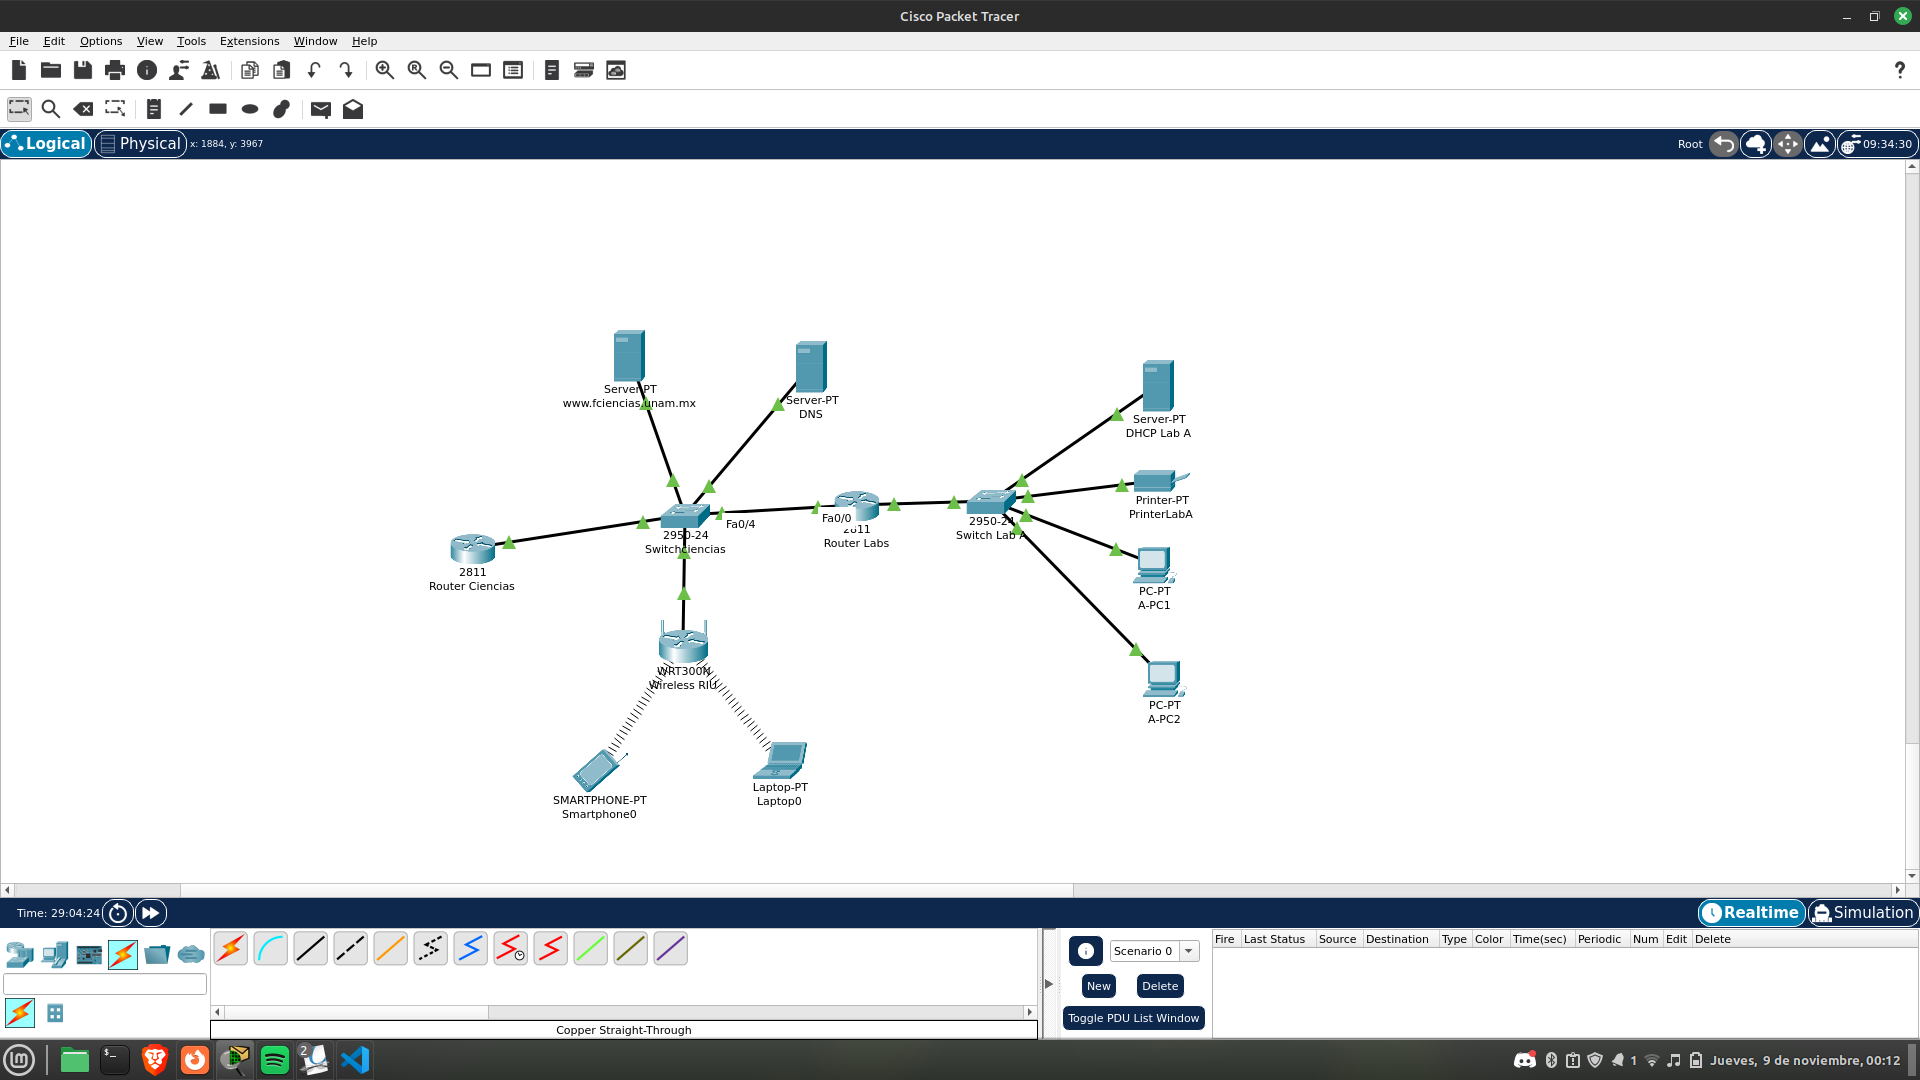
\includegraphics[width=12cm, height=8cm]{images/router ciencias.png}\\

Antes de pasar con el siguiente punto primero debemos de modificar el servidor dns de ciencias, cambiandole el nombre y agregando su DNS:\\

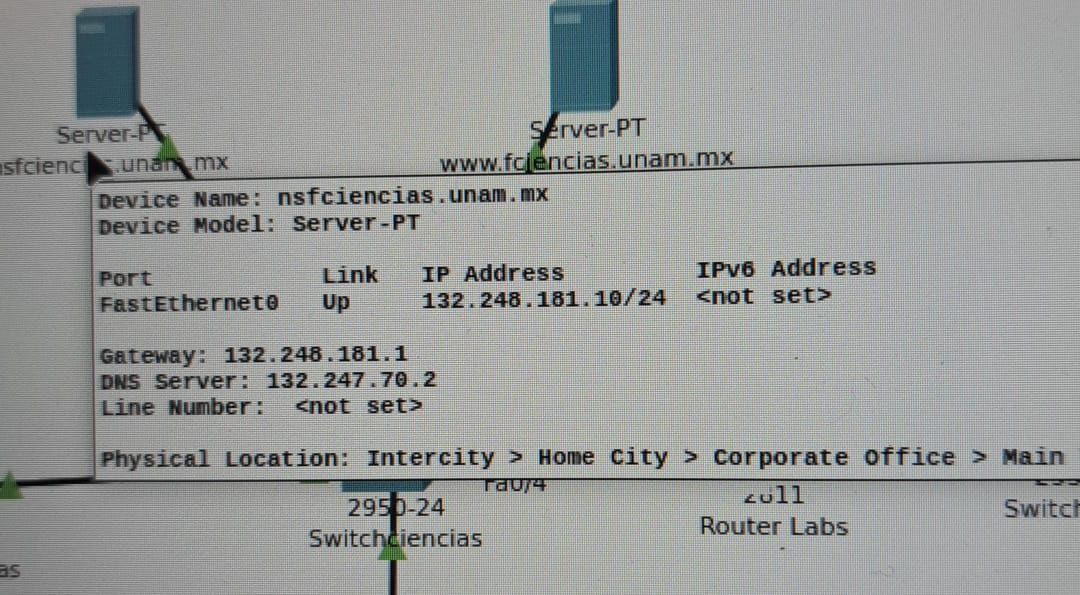
\includegraphics[width=12cm, height=8cm]{images/dns c5enc5as.jpeg}\\


{\color{red} \subsubsection*{\textbf{Red DGTIC}}}
\vspace{1em}

La red de DGTIC se divide en 2 partes:\\
\begin{enumerate}
  \item Red de equipos
  \item Red de servidores
\end{enumerate}

iniciaremos tomando como referencia la imagen 1 de el pdf de instrucciones, configuraremos primero todos los revidores de la red de DGTIC.\\

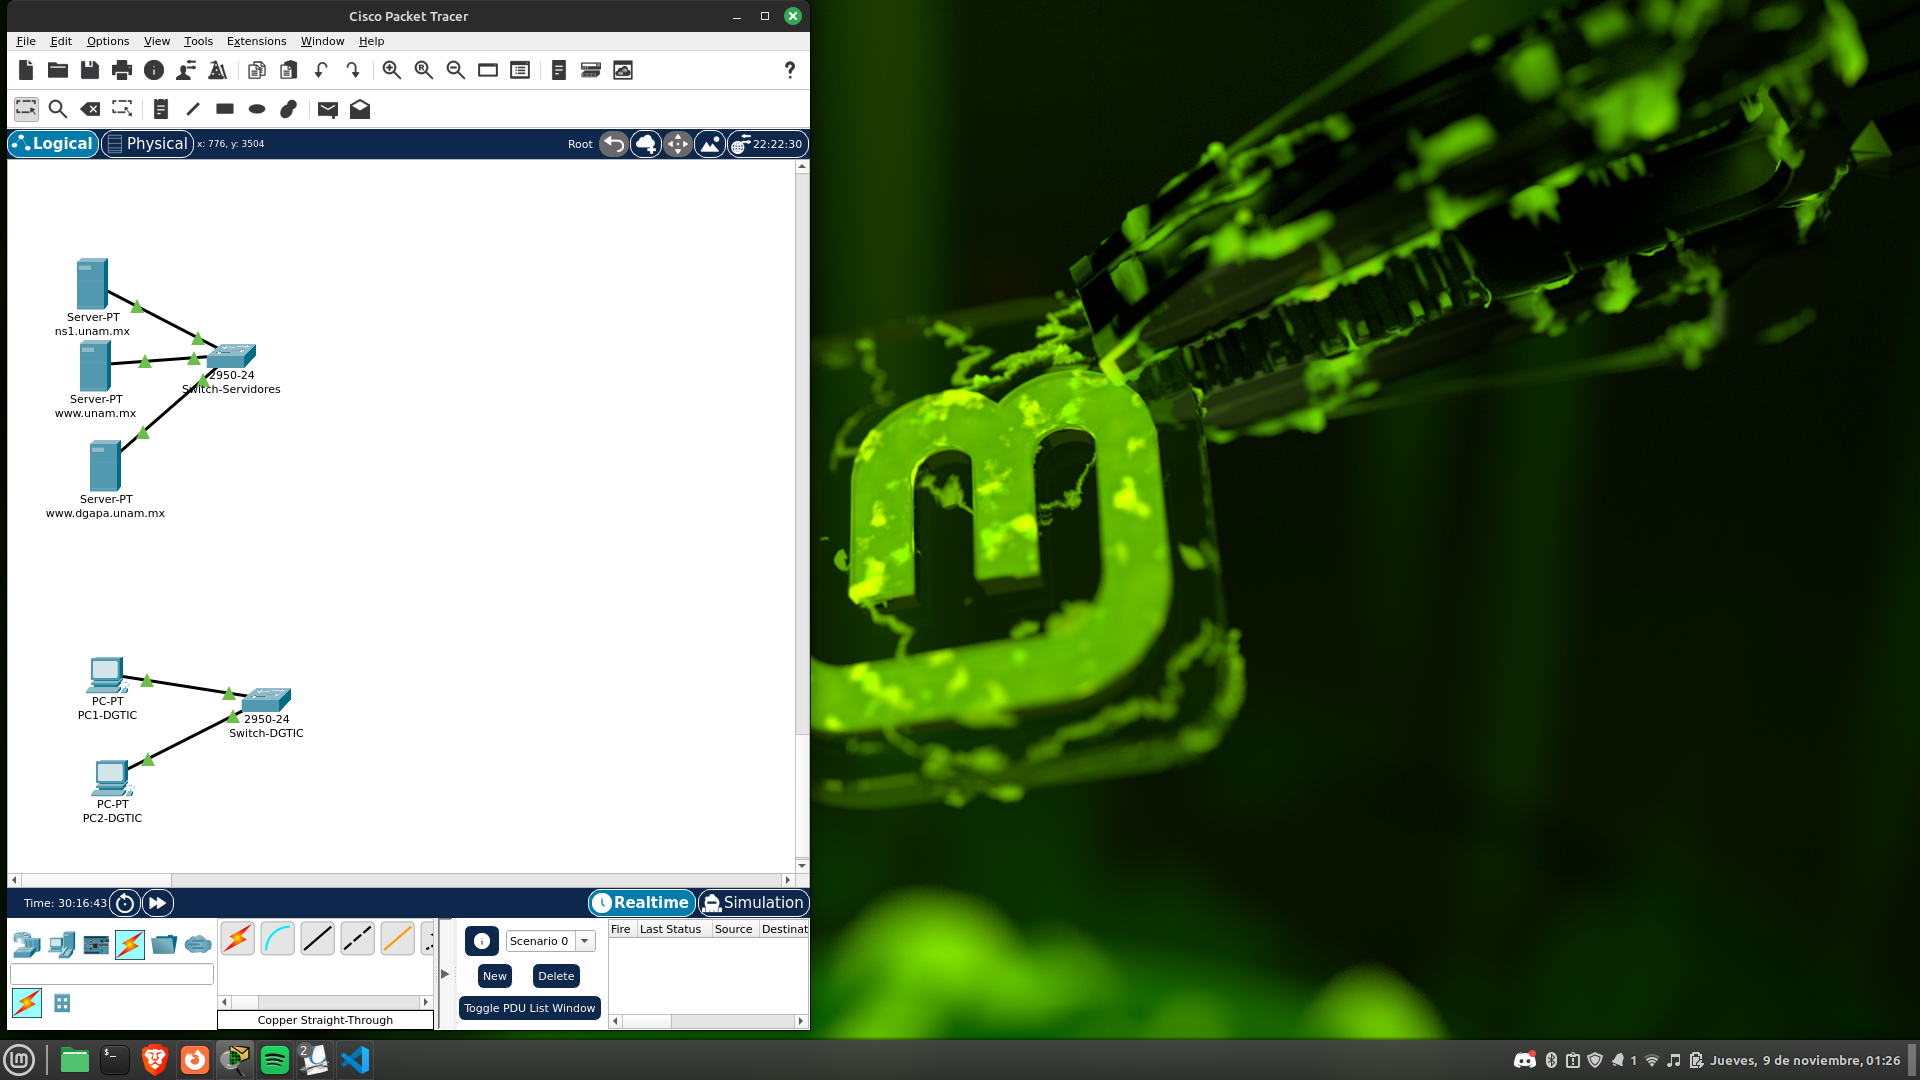
\includegraphics[width=12cm, height=8cm]{images/redesdgtic.png}\\


{\color{red} \subsubsection*{\textbf{Configuración de los sitios Web}}}
\vspace{1em}

Configuramos el index para que muestre en pantalla lo siguiente:\\

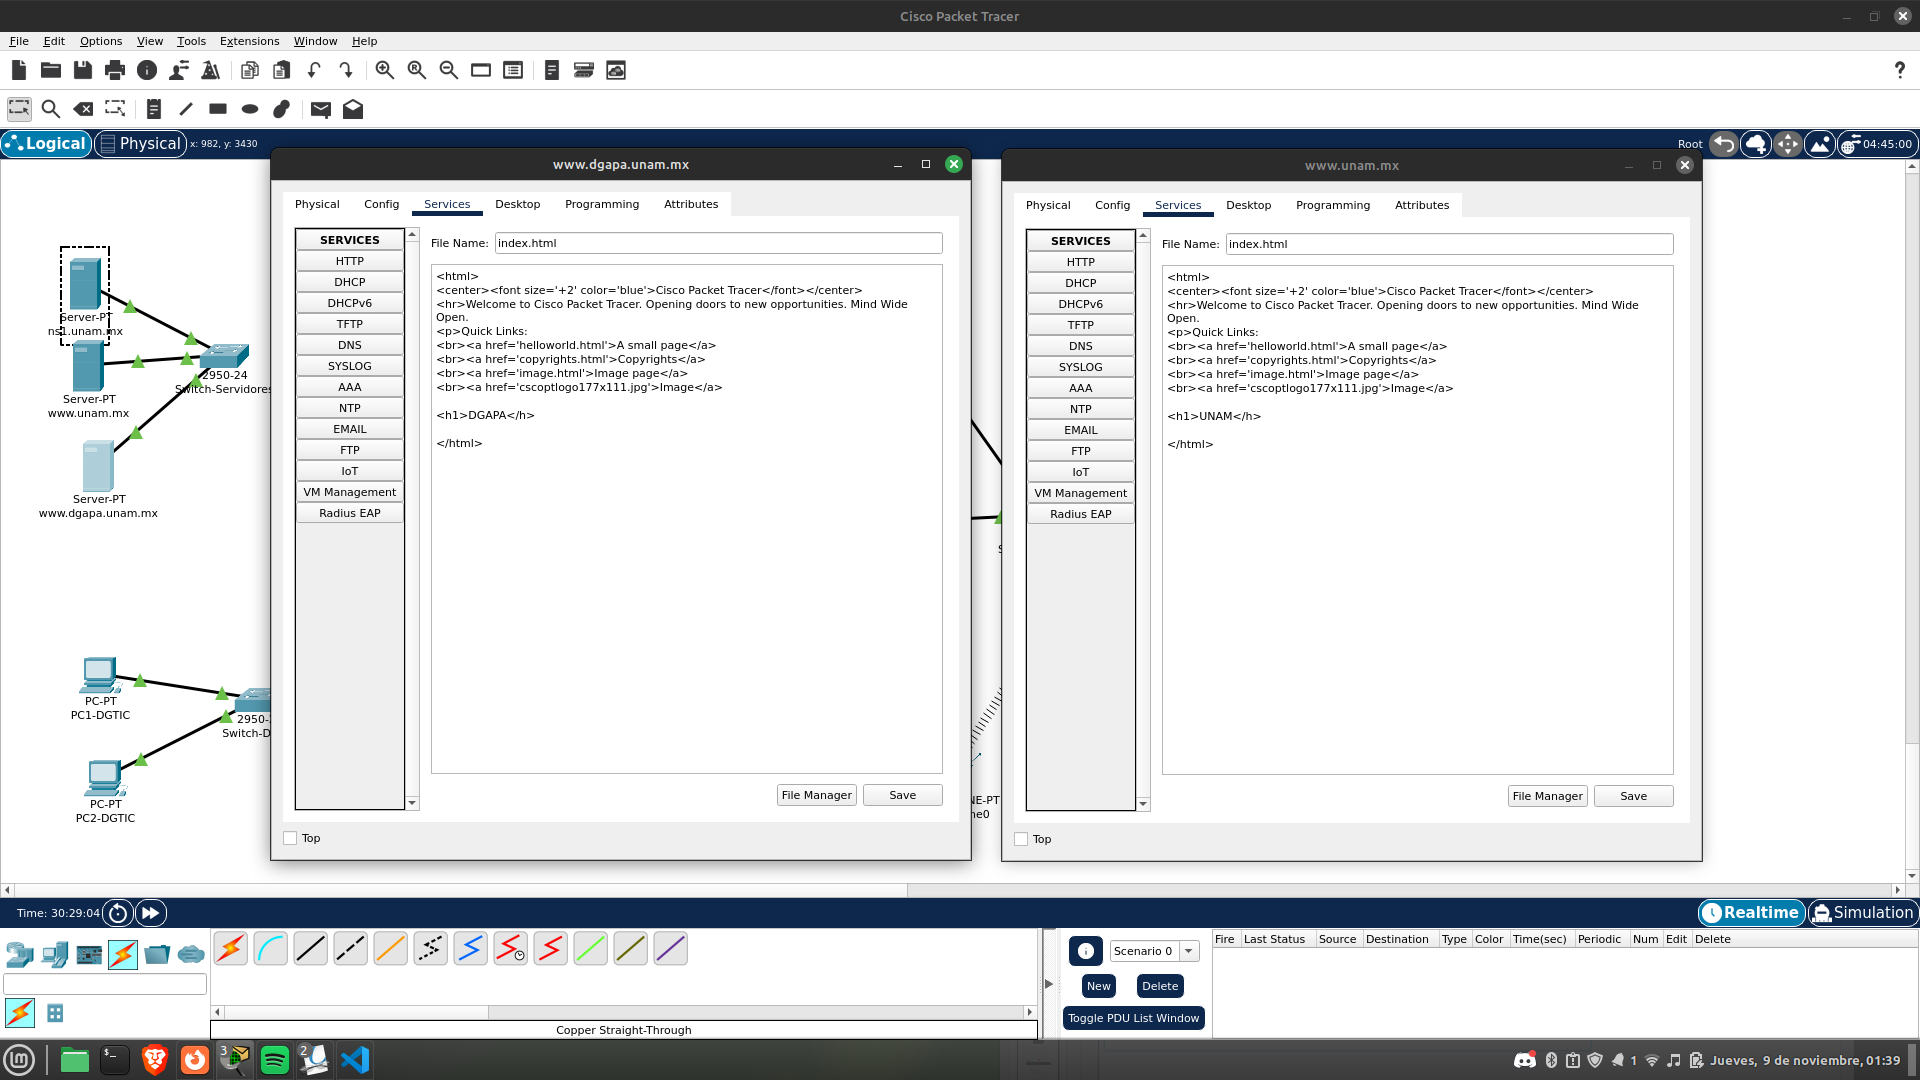
\includegraphics[width=12cm, height=8cm]{images/confweb.png}\\

{\color{red} \subsubsection*{\textbf{Configuración de registros DNS}}}
\vspace{1em}

Despues de configurar los registros de los servidores DNS, quedan de la siguiente manera: (cabe mencionar que no es similar al pdf de la practica porque hay unos de fisica que hasta el momento no se han mencionado.)\\

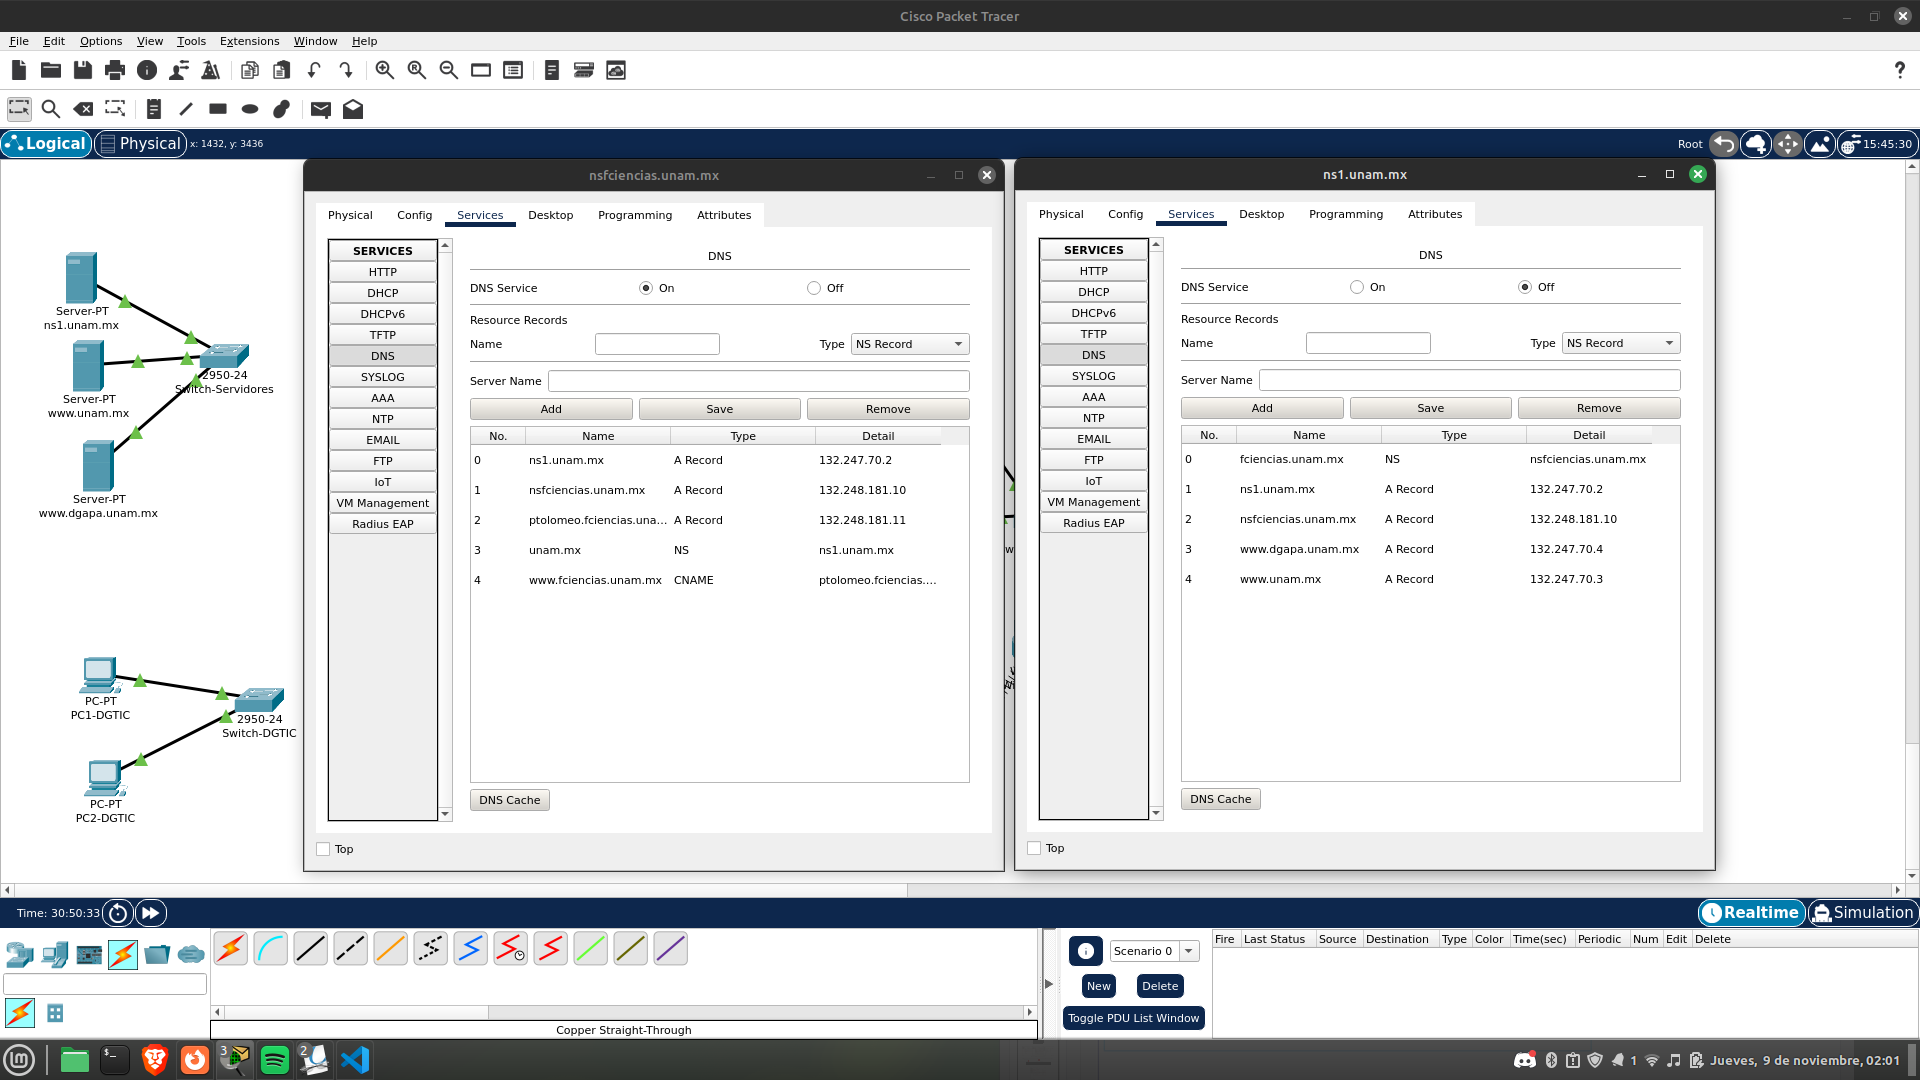
\includegraphics[width=12cm, height=8cm]{images/registros dns.png}\\

agregamos los registros SOA:\\

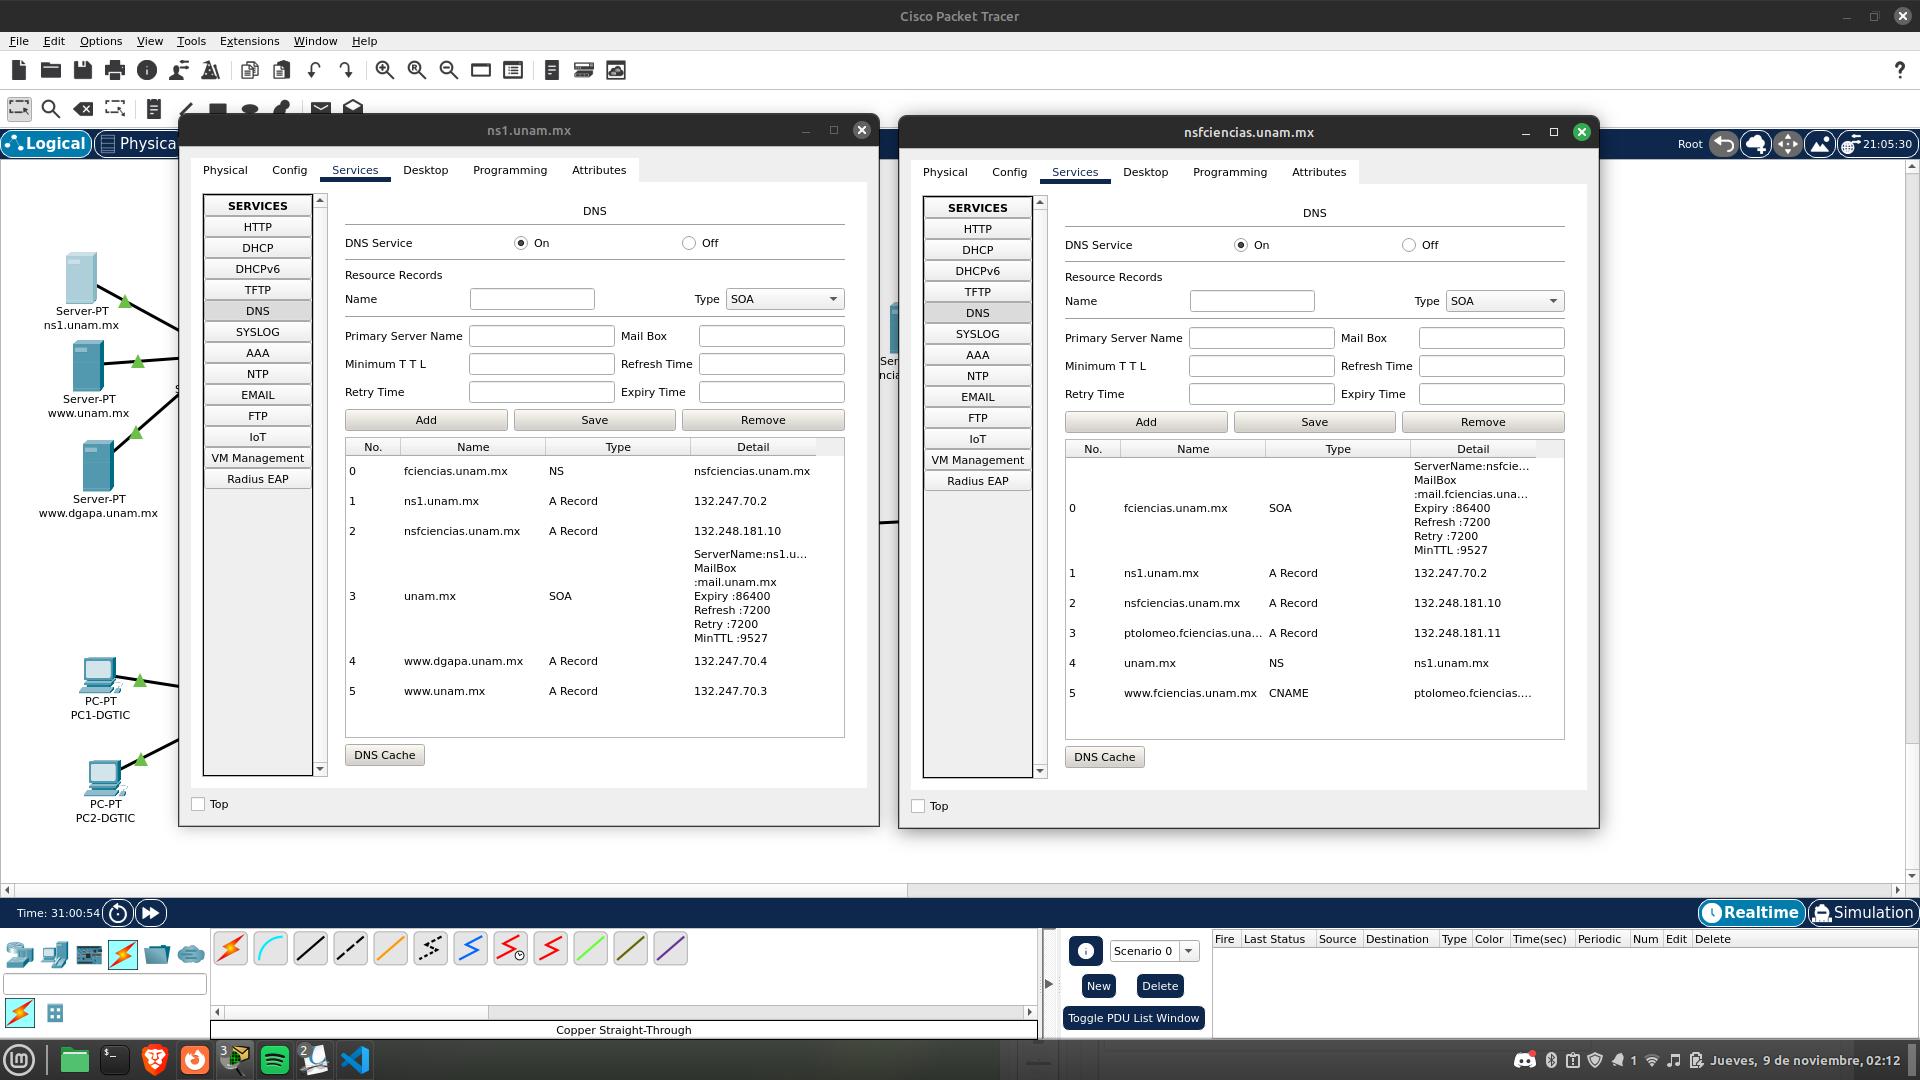
\includegraphics[width=12cm, height=8cm]{images/soa.png}\\

{\color{red} \subsubsection*{\textbf{Configuración de los router}}}
\vspace{1em}

configuramos los routers y uno que sera el grande que además
tiene capacidades de un dispositivo de capa 3, es necesario desactivar la función de que
solamente la interfaz Ethernet funcione como si fuera de un Switch, para que se le
pueda asignar una dirección IP a dicha interfaz.\\

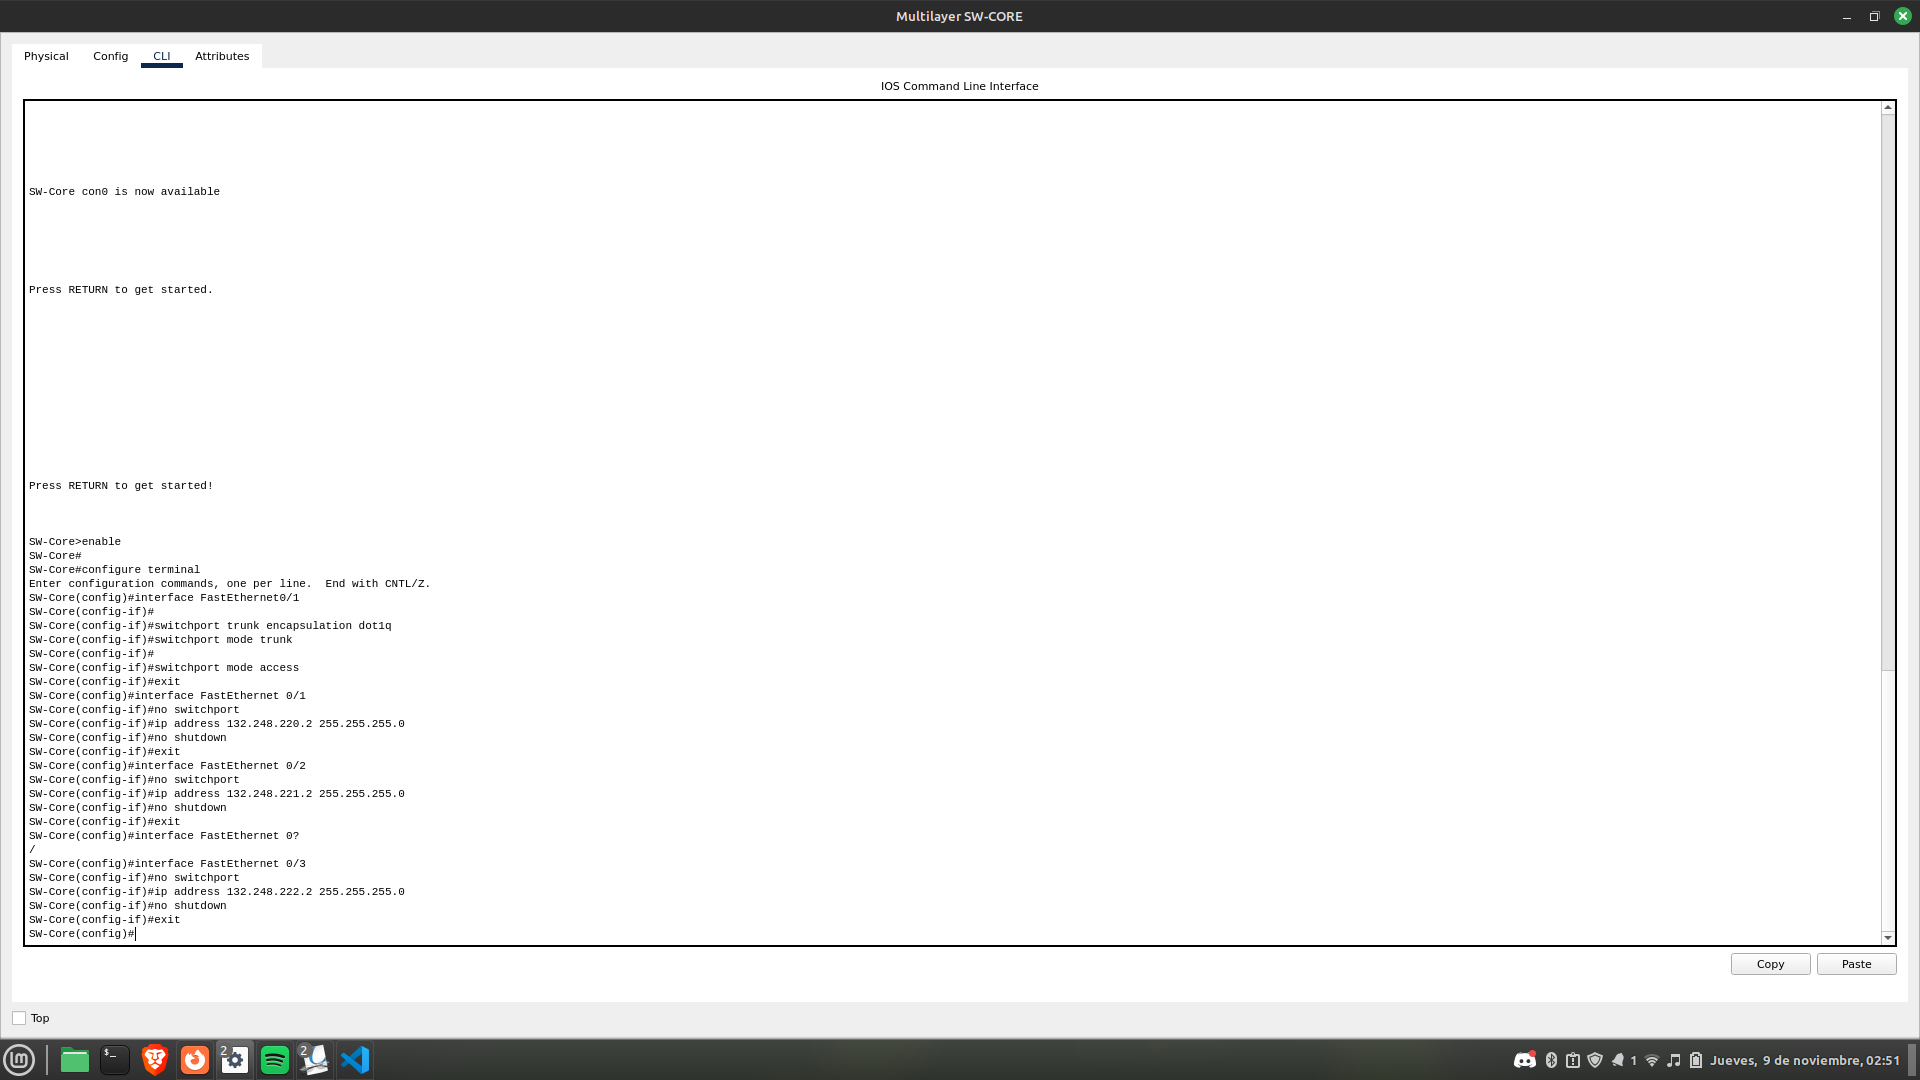
\includegraphics[width=12cm, height=8cm]{images/router grandote.png}\\

{\color{red} \subsection*{\textbf{ Configuraciones al reporte}}}
\vspace{1em}

Como no se ha configurado la ruta que se debe tomar para conectarse a cada uno de los
servidores webs (desde cualquier punto de la red) no será posible acceder desde cualquier
ubicación a estos sitios web, de cada red. Esto se definirá en la siguiente práctica por medio
del ”ruteo dinámico”.\\

{\color{red} \subsubsection*{\textbf{  Mostrar en el reporte por cada Router y el SW-Core, la salida de los comandos:}}}
\vspace{1em}

\begin{enumerate}
  \item $Router\#show ip route$
  \item $Router\#show ip interface brief$
\end{enumerate}


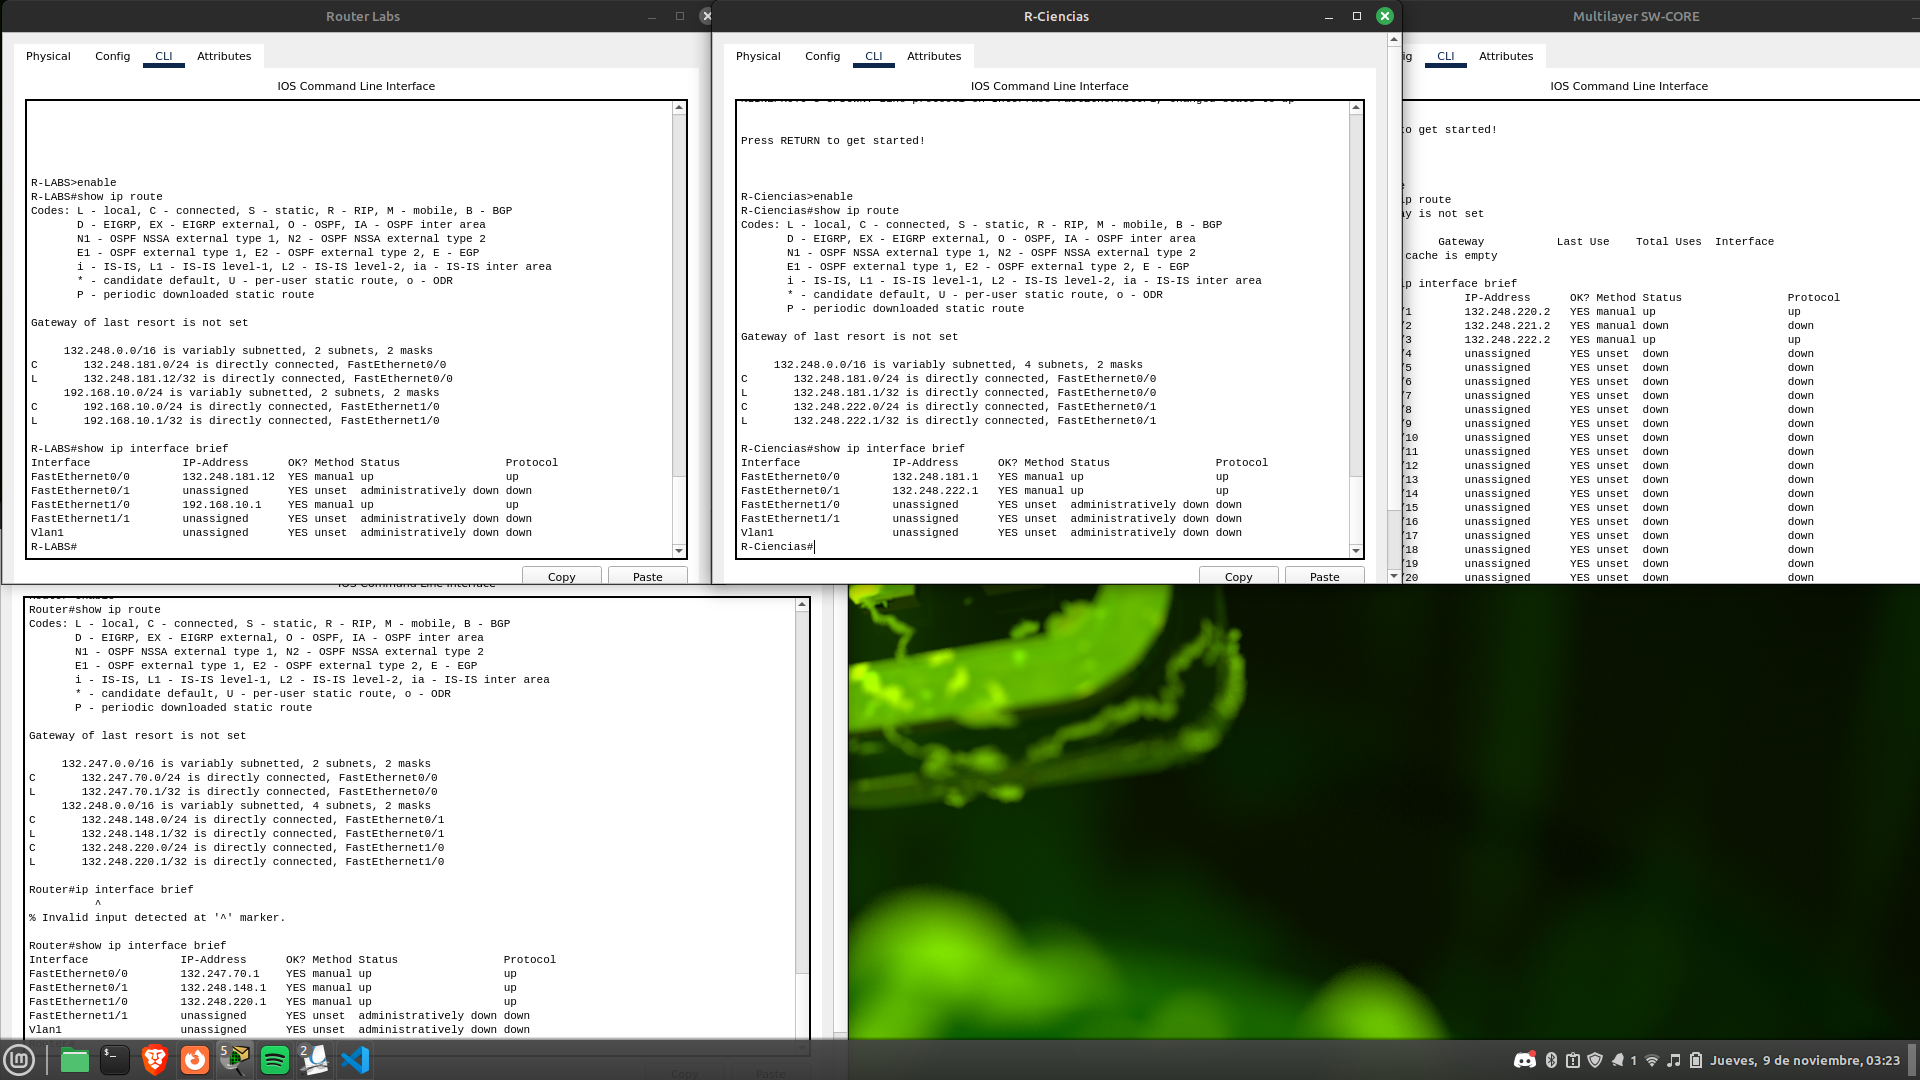
\includegraphics[width=12cm, height=8cm]{images/finaaaaal routers.png}\\

{\color{red} \subsubsection*{\textbf{Mostrar en el reporte que se puede acceder desde las siguientes ubicaciones:}}}
\vspace{1em}

Anexamos las capturas, con la nota que se puede ver en la parte de arriba de la pestaña en que dispositivo es donde estamos haciendo la busqueda.\\

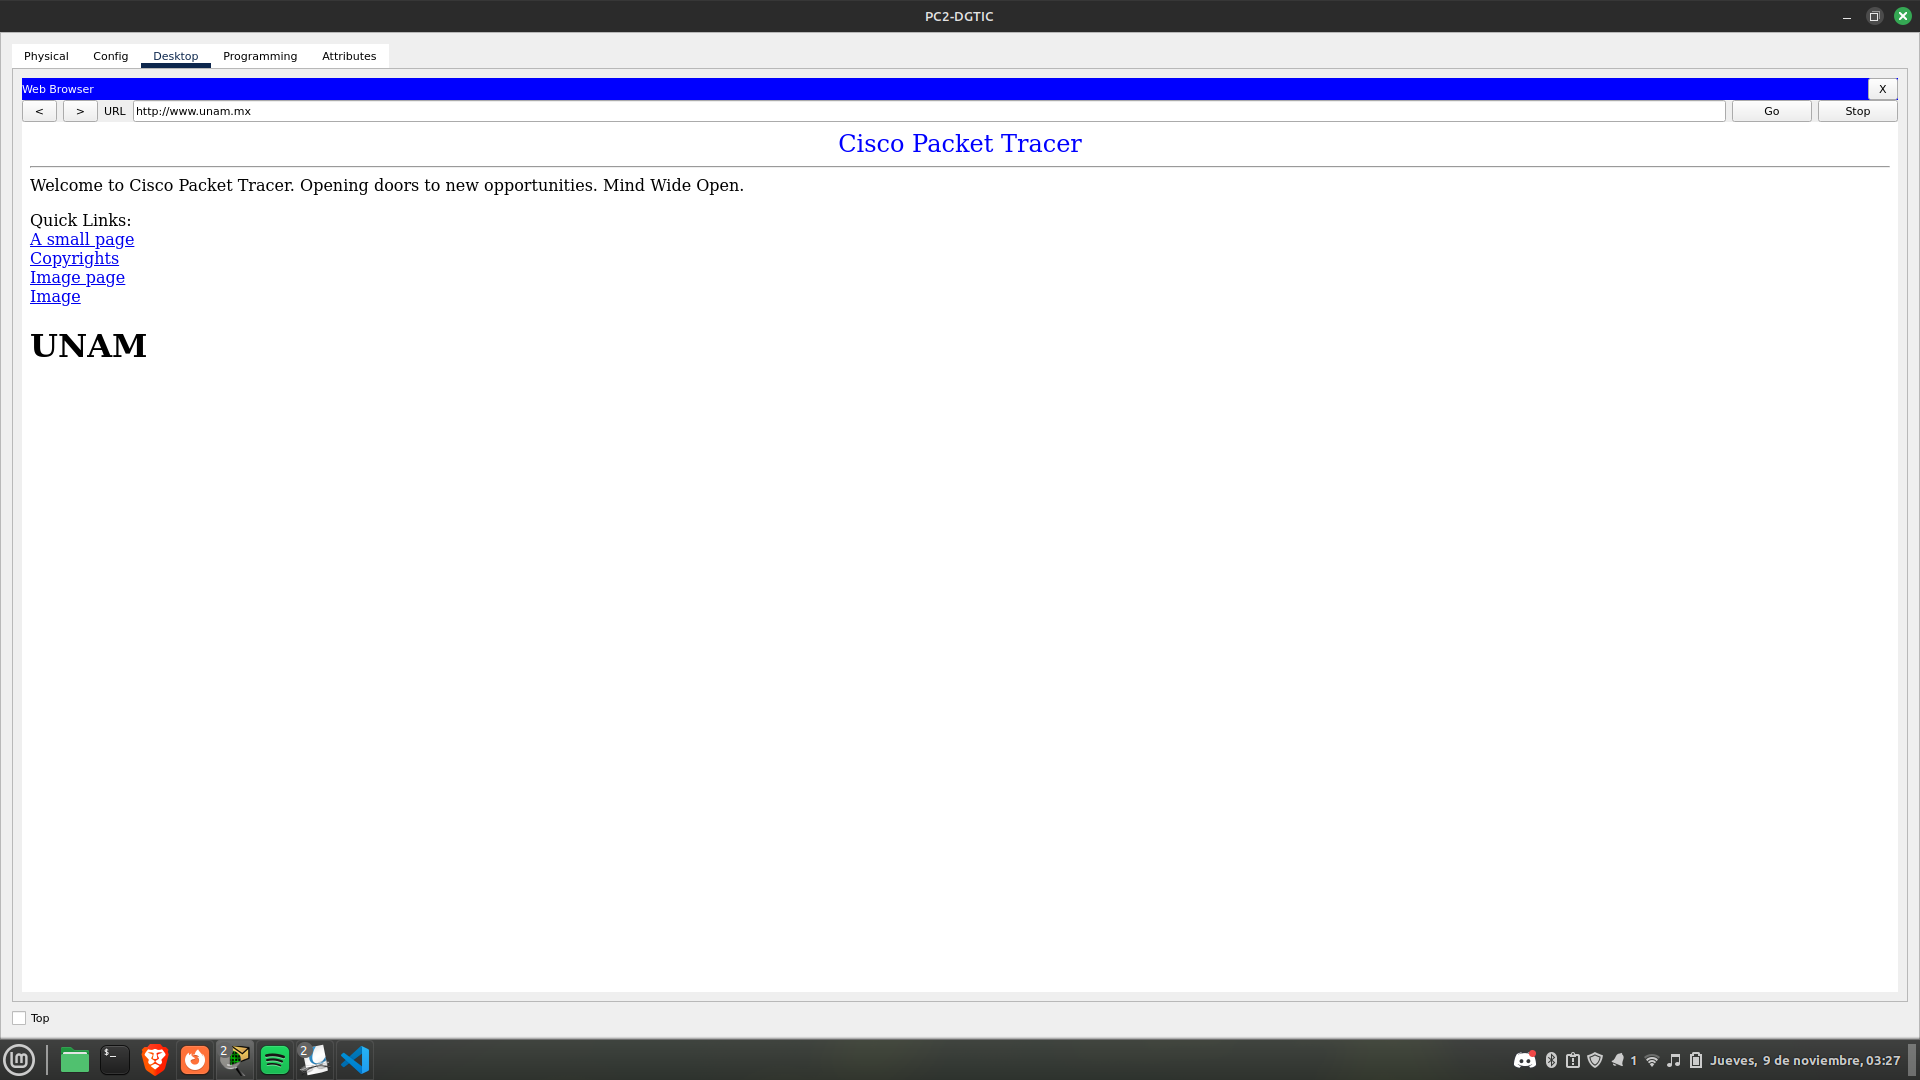
\includegraphics[width=12cm, height=8cm]{images/pc2-unam.png} UNAM EN PC2\\

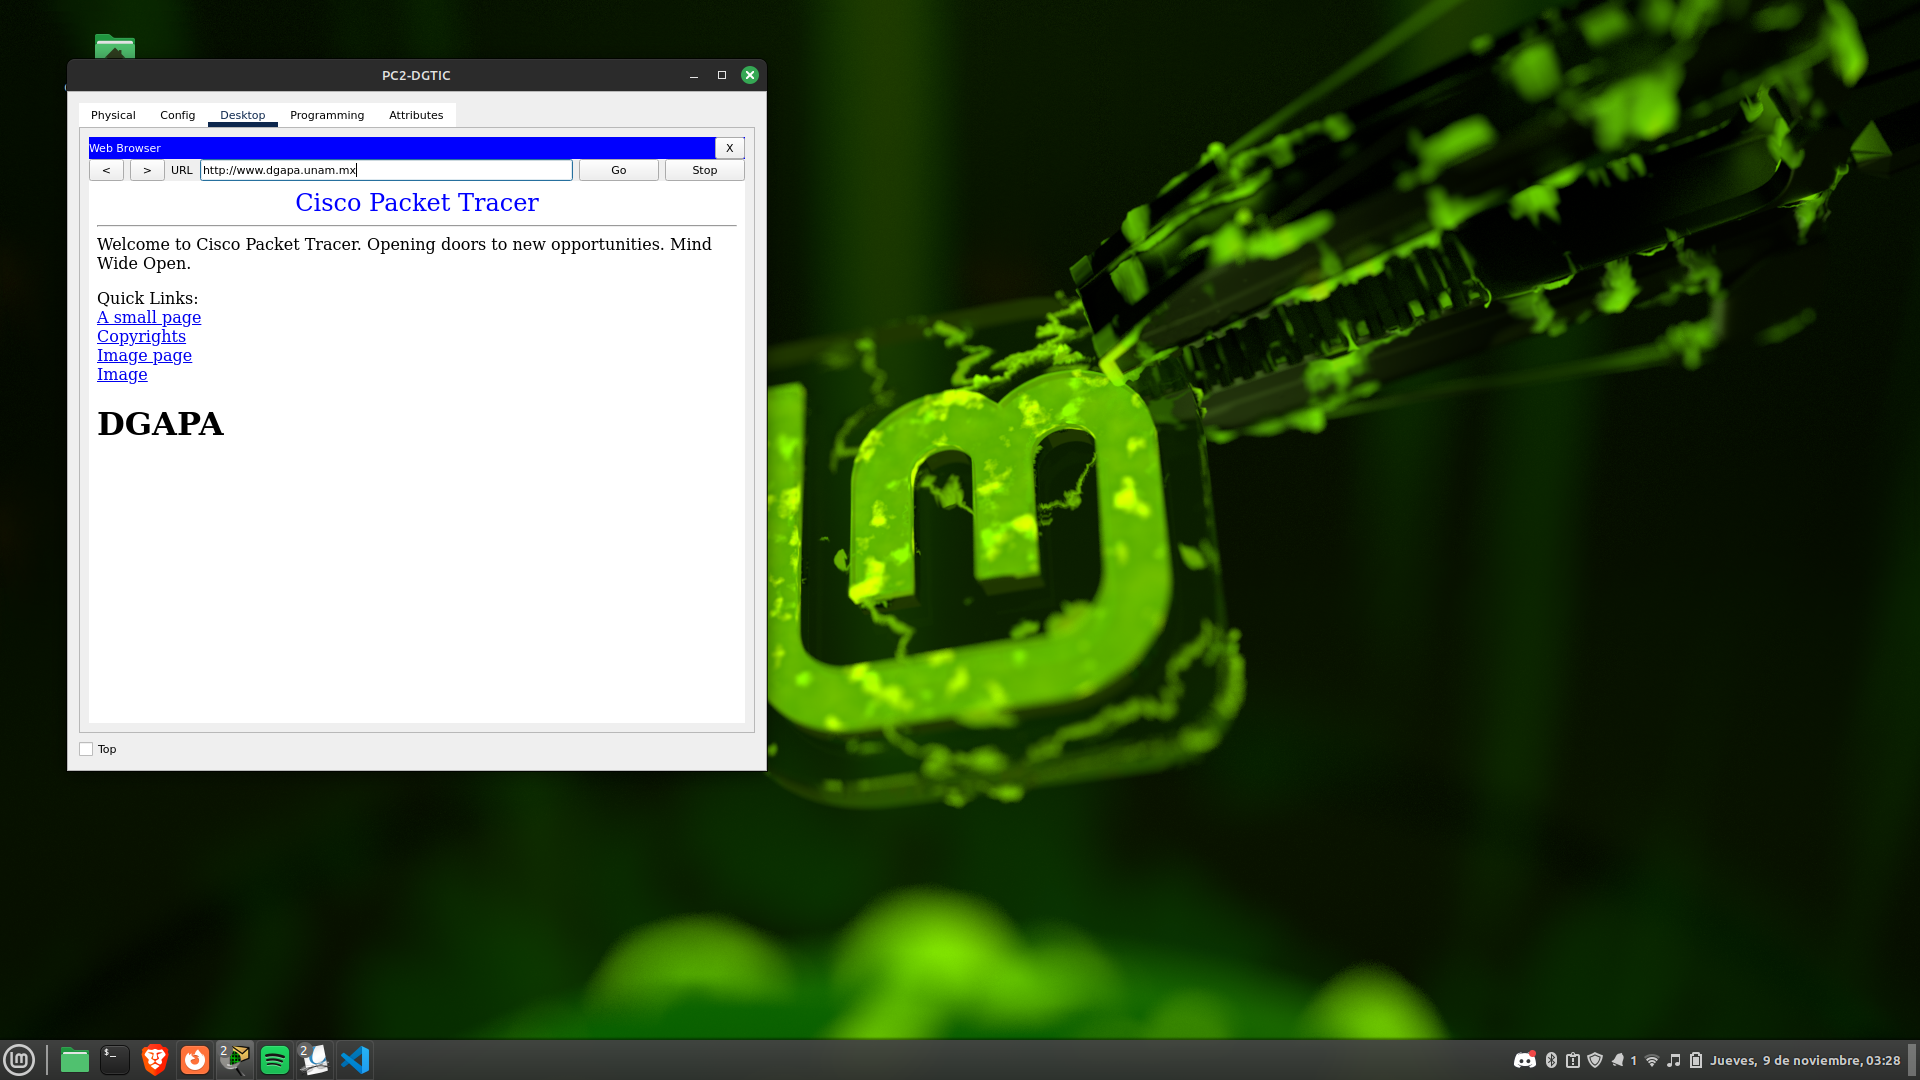
\includegraphics[width=12cm, height=8cm]{images/pc2-dgapa.png}DGAPA EN PC2\\

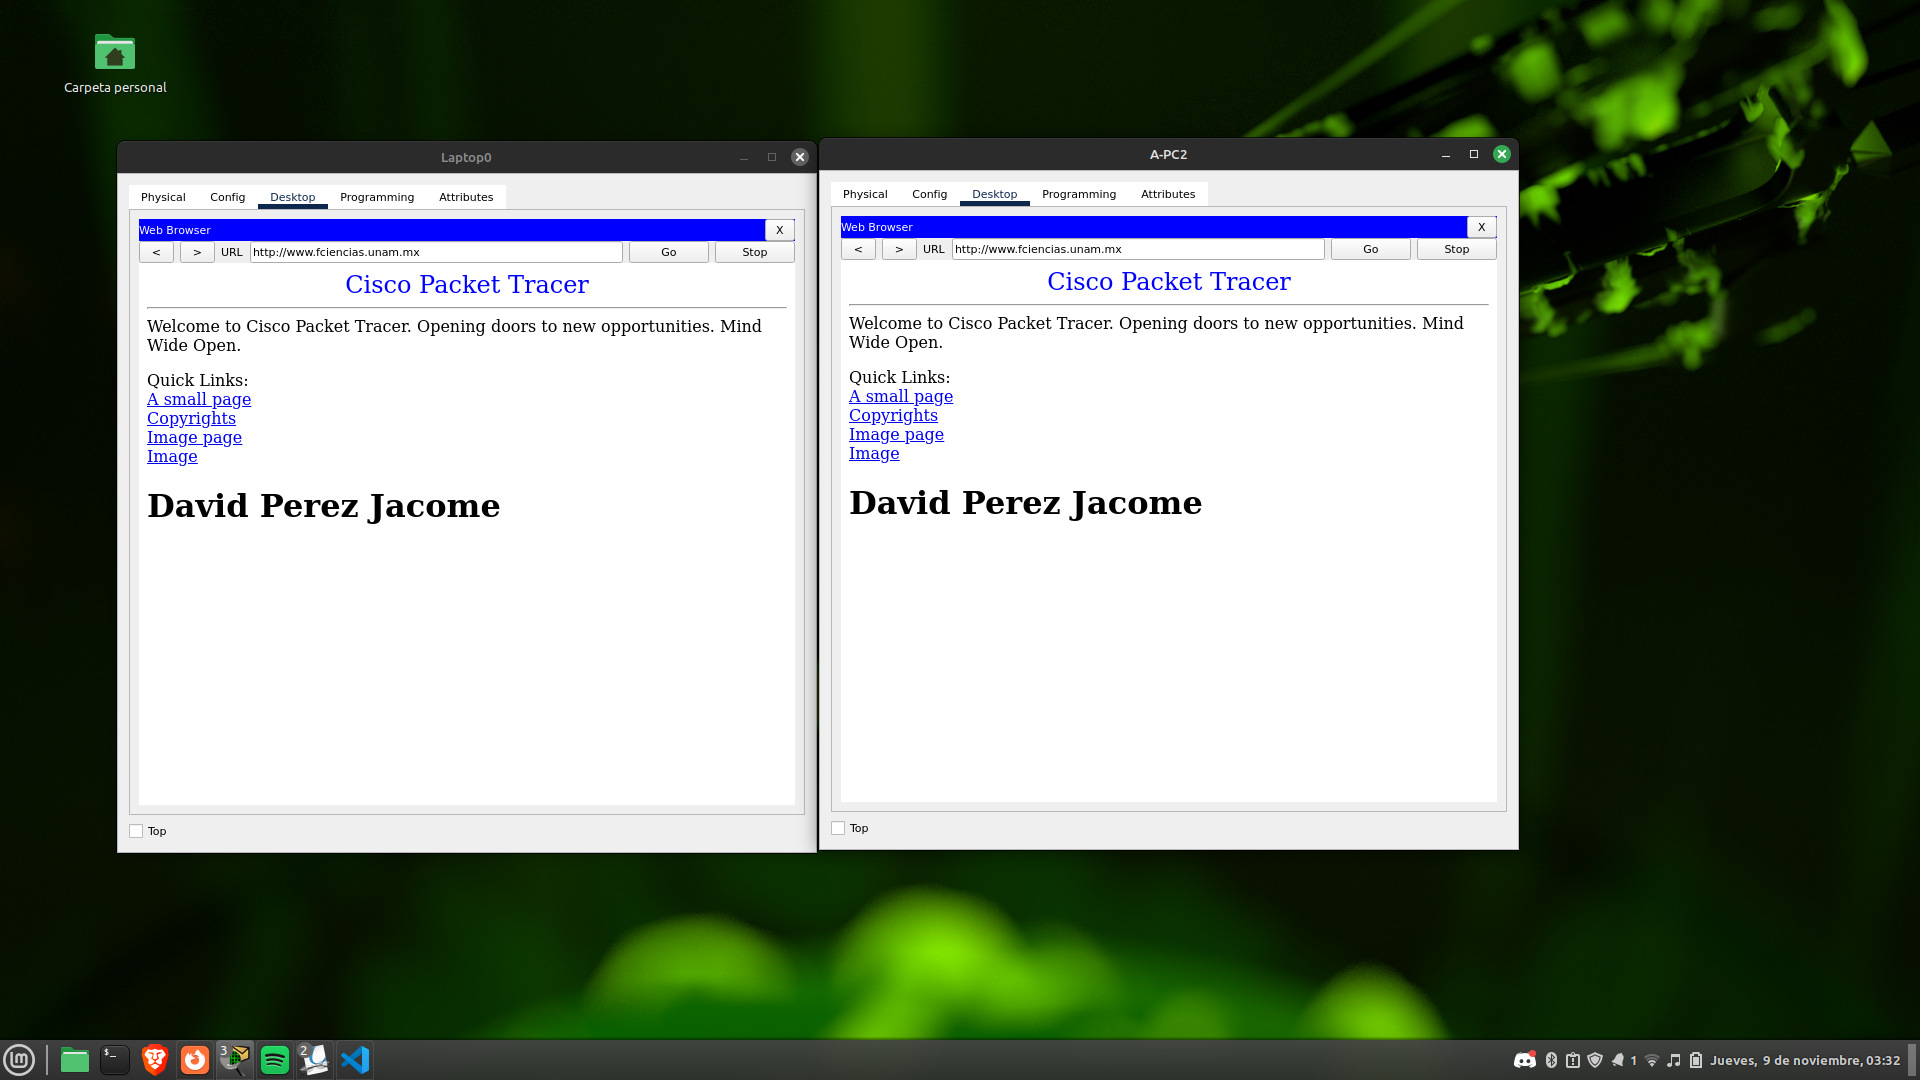
\includegraphics[width=12cm, height=8cm]{images/lap y lab.png}LAB Y LAPTOP\\

{\color{red} \subsubsection*{\textbf{Mostrar la memoria caché de cada servidor DNS después de haber accedido a los sitios web:}}}
\vspace{1em}

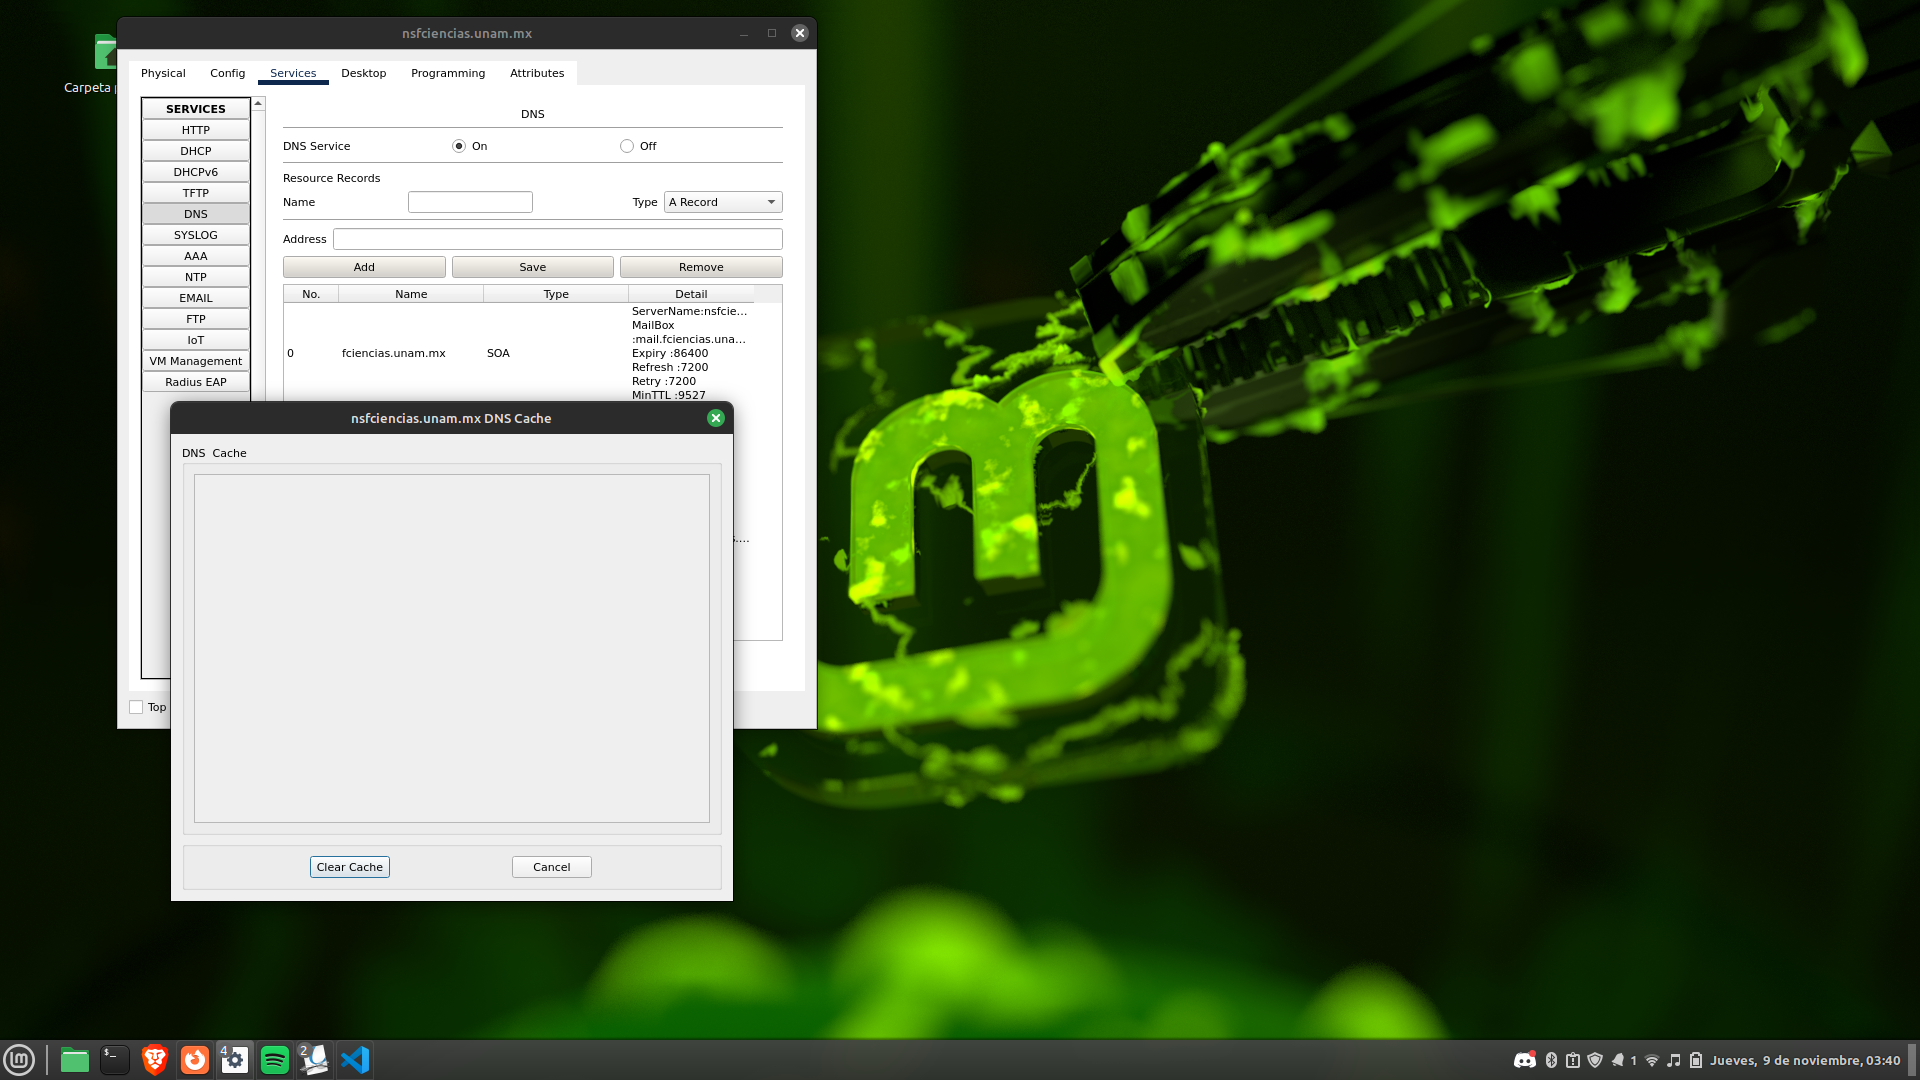
\includegraphics[width=12cm, height=8cm]{images/CACHE1.png}\\

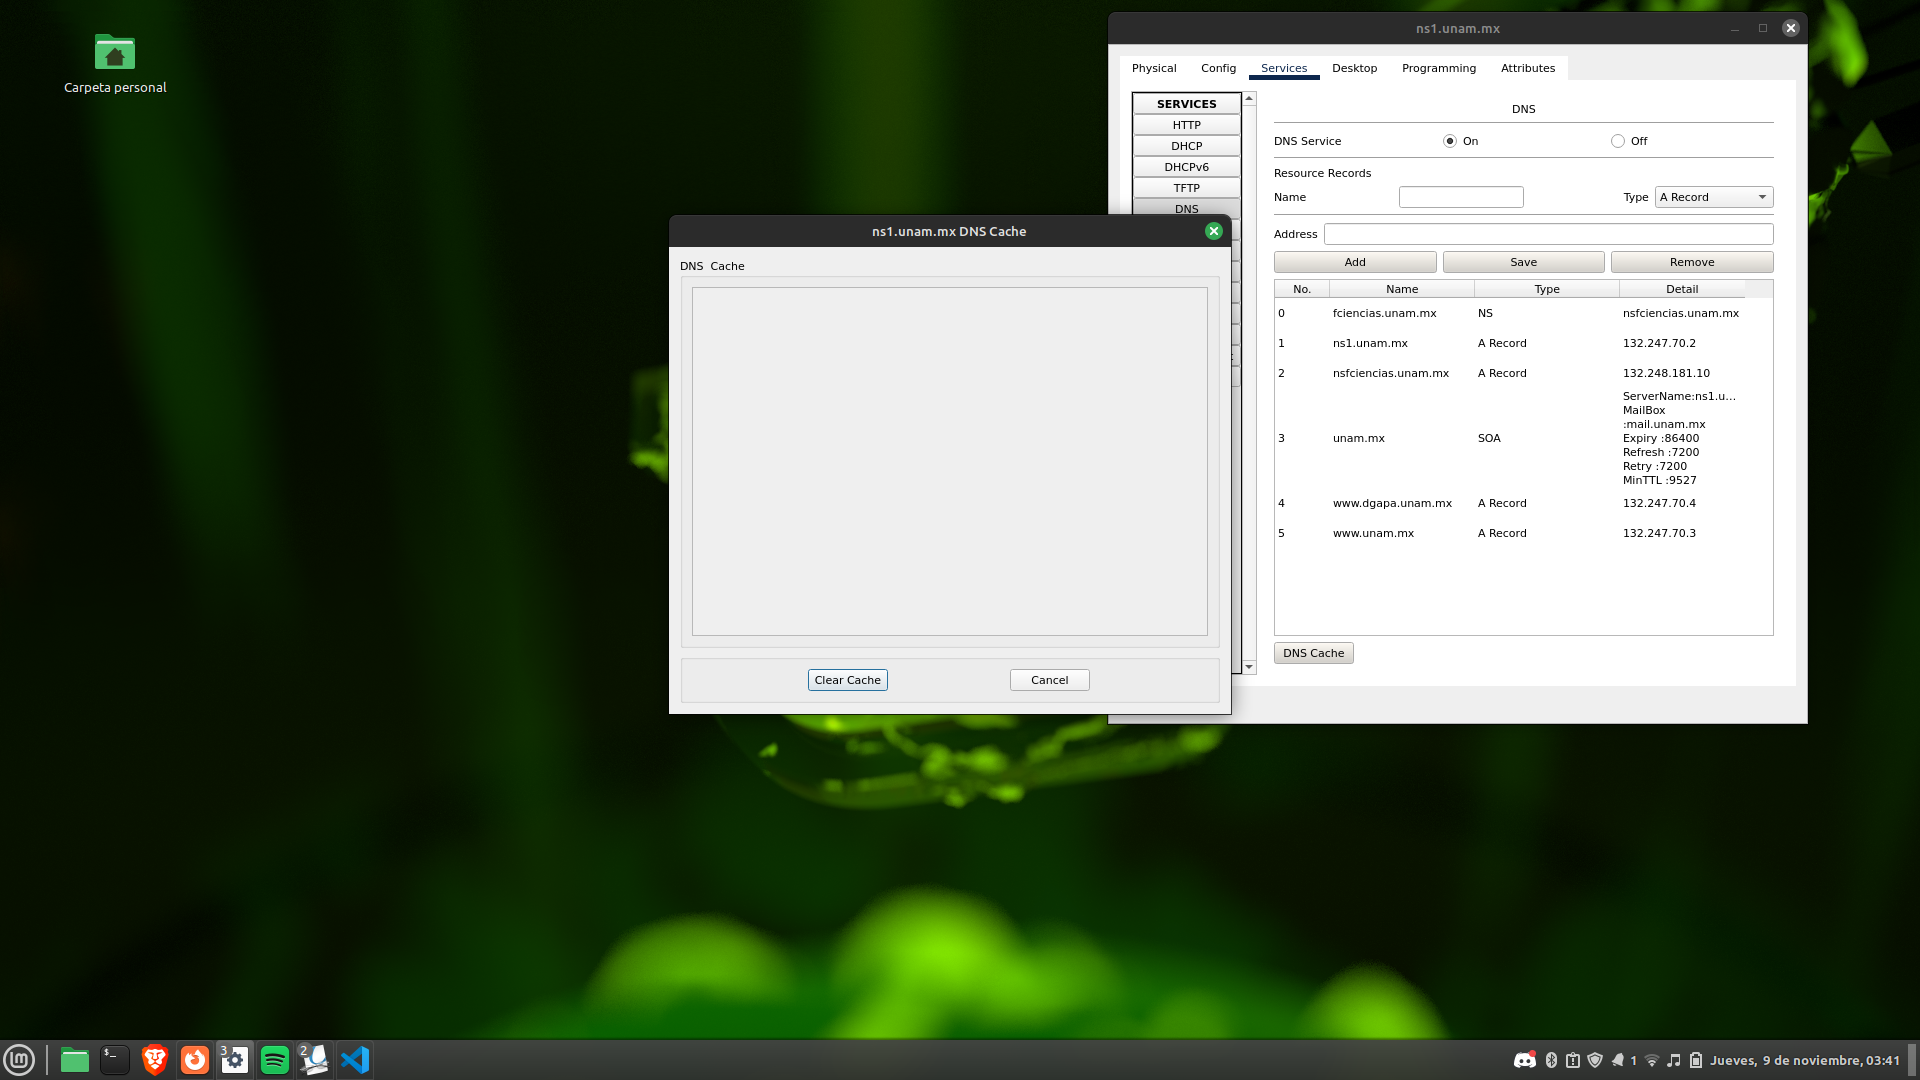
\includegraphics[width=12cm, height=8cm]{images/CACHE2.png}\\

{\color{red} \subsubsection*{\textbf{CUESTIONARIO:}}}
\vspace{1em}

\begin{enumerate}
  \item ¿Qué direcciones IP le asignó el Router inalámbrico a cada host, a la Laptop y al
  smartphone, conectados a la red inalámbrica RIU?\\
  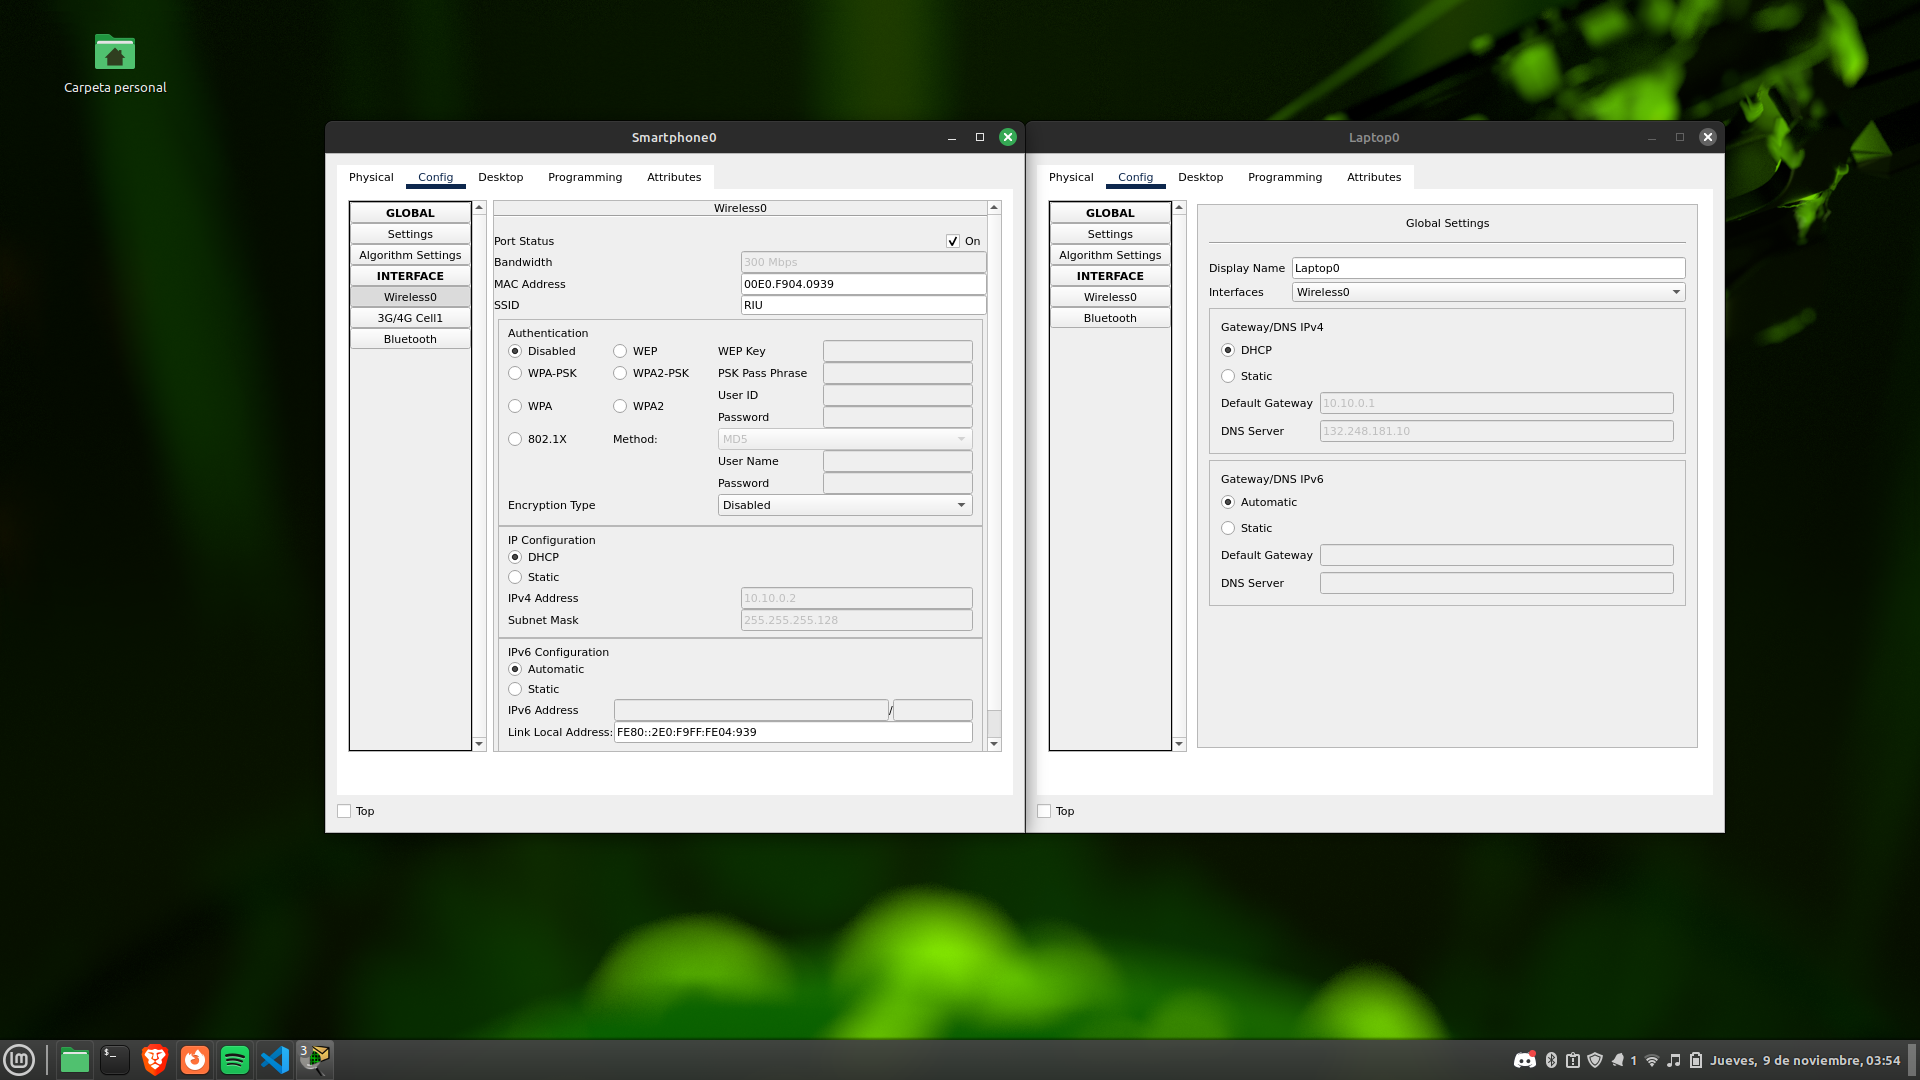
\includegraphics[width=12cm, height=8cm]{images/ip de lap y cel .png}
  \item ¿Qué direcciones IP le asignó el servidor DHCP a cada host de la red del Laboratorio A?\\
  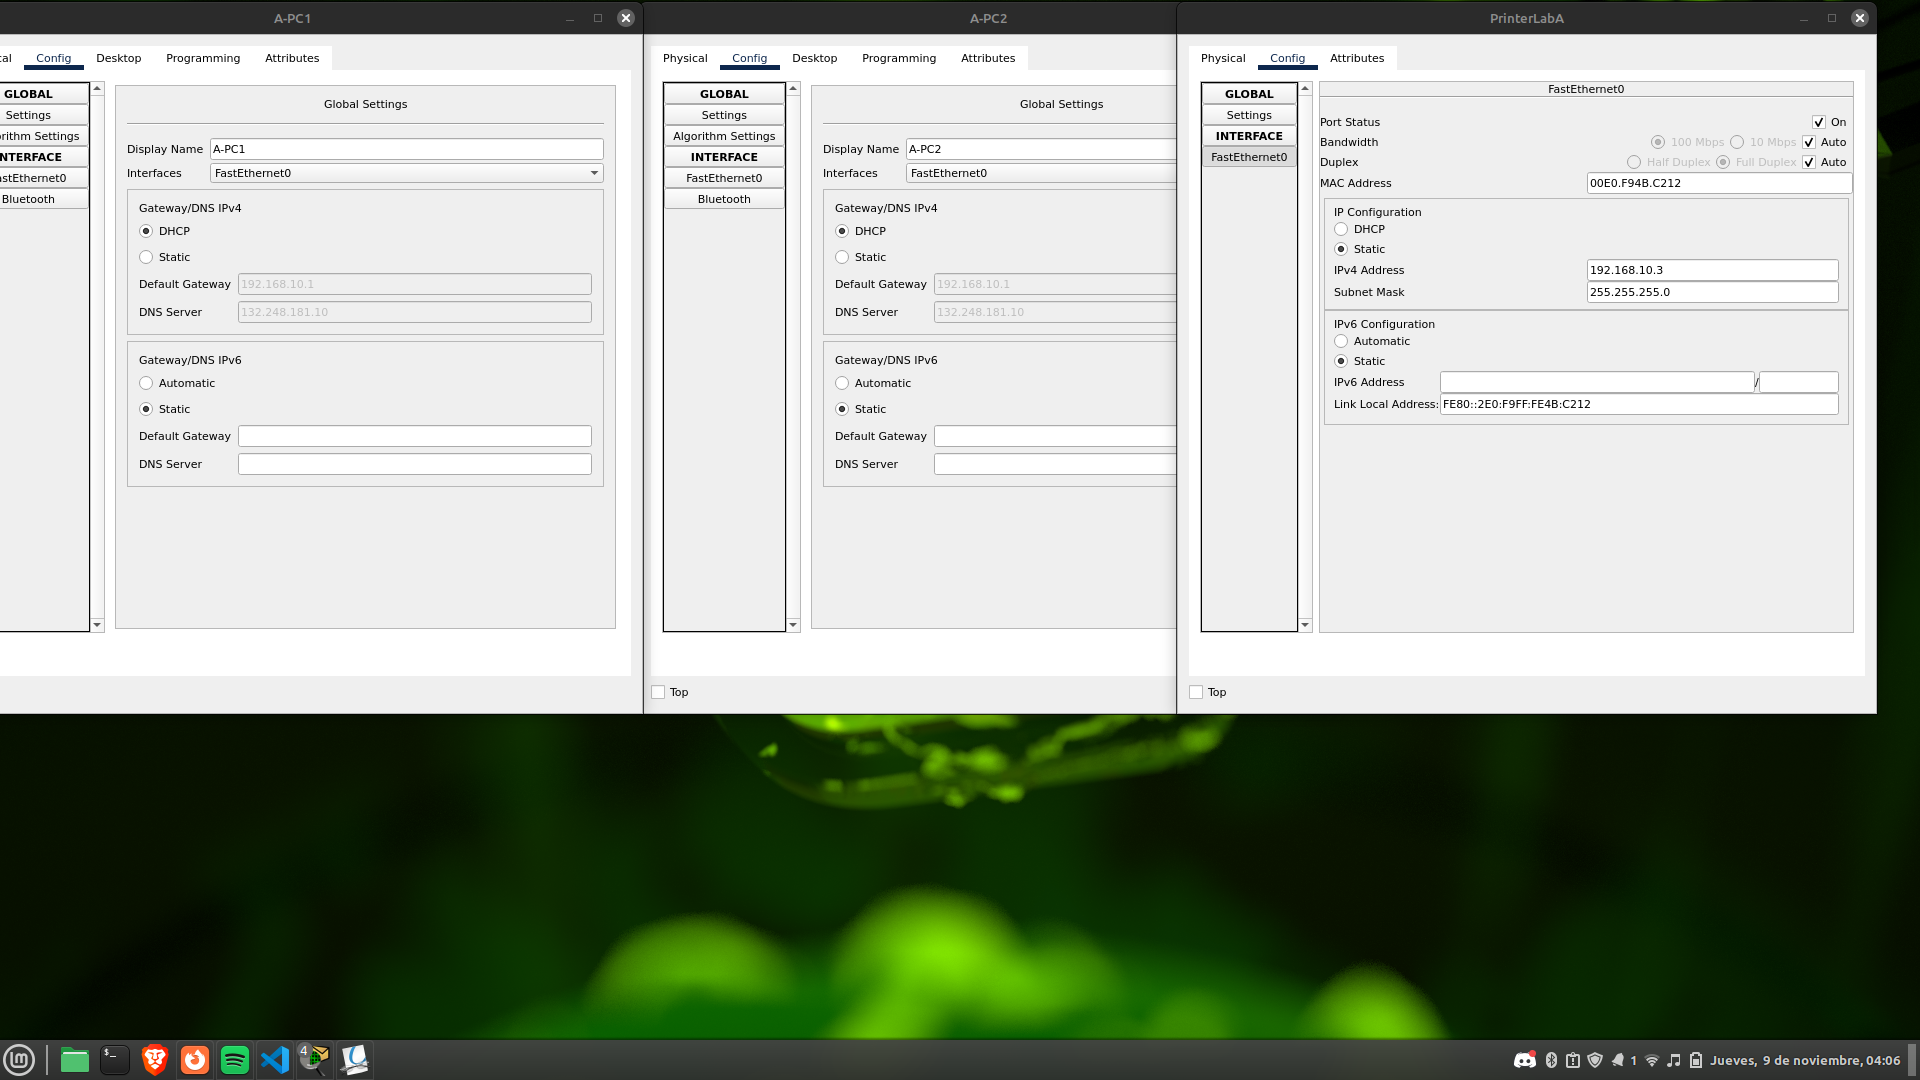
\includegraphics[width=12cm, height=8cm]{images/pregunta2.png}
  \item Investigue el concepto de DHCP y explique.\\
  \textbf{Protocolo de Configuración Dinámica de Hosts, es un protocolo de red utilizado para asignar de manera automática direcciones IP y otros parámetros de configuración de red a dispositivos en una red, como computadoras, impresoras y dispositivos móviles}
  \item  Investigue los conceptos de NAT y PAT, y explique.\\
  \textbf{NAT (Network Address Translation) y PAT (Port Address Translation) son técnicas utilizadas en redes de computadoras para permitir que múltiples dispositivos en una red privada compartan una única dirección IP pública, NAT permite que un enrutador o dispositivo de red traduzca las direcciones IP privadas de los dispositivos en una red local a una única dirección IP pública, mientras que PAT es una extensión de NAT que permite que múltiples dispositivos en una red privada compartan una única dirección IP pública utilizando diferentes números de puerto.}
  \item ¿Qué es la máscara de red o Netmask?\\
  \textbf{Es  un número de 32 bits que se utiliza junto con una dirección IP para definir la parte de la dirección IP que identifica la red y la parte que identifica los dispositivos específicos en esa red}
  \item ¿Qué es la Puerta de Enlace predeterminada o Default Gateway?\\
  \textbf{Es el dispositivo (generalmente un router) en una red de computadoras que actúa como el punto de salida para el tráfico que se dirige fuera de la red local hacia otras redes o hacia Internet.}
  \item ¿Qué es el SSID en una red inalámbrica?\\
  \textbf{Simplemente  es un nombre único que identifica una red inalámbrica. Es básicamente el nombre de la red Wi-Fi a la que los dispositivos se pueden conectar para acceder a Internet o a otros recursos en una red local.}
  \item  ¿Cuáles son las funciones de un router en una red de computadoras?\\
  \textbf{Algunas de sus funciones son,Enrutamiento de Datos, Interconexión de Redes, Puerta de Enlace Predeterminada, NAT y PAT, Seguridad, Calidad de Servicio (QoS), Gestión de Ancho de Banda,VPN (Redes Privadas Virtuales)}
  \item ¿Qué son los protocolos de ruteo?\\
  \textbf{Los protocolos de ruteo son conjuntos de reglas y algoritmos que los routers utilizan para determinar la mejor ruta o camino para enviar datos desde su origen hasta su destino a través de una red de computadoras.}
  \item ¿Qué es una ruta estática en un router?\\
  \textbf{Una ruta estática en un router es una entrada manualmente configurada en la tabla de enrutamiento del router para indicar cómo alcanzar una red específica o una dirección IP de destino.}
  \item Indique para que se usan los registros A, NS, CNAME y SOA en un servidor DNS\\
  \textbf{A: se utiliza para asociar un nombre de dominio con una dirección IP específica.
  NS: se utiliza para especificar los servidores de nombres autoritativos para un dominio. Estos servidores de nombres son responsables de almacenar información sobre ese dominio específico.
  CNAME: se utiliza para crear alias o apodos para nombres de dominio. Permite que un nombre de dominio tenga múltiples nombres asociados a la misma dirección IP.
  SOA: contiene información autoritativa sobre el dominio, incluyendo el nombre del servidor primario, la dirección de correo electrónico del administrador del dominio, la versión del archivo de zona y varios valores de temporización que controlan la frecuencia de actualización de la información de la zona.}
\end{enumerate}





\end{document}